\documentclass[graybox,envcountchap]{svmono}
\usepackage{amsmath,amssymb,graphicx,pstricks,makeidx}
\usepackage{mathptmx,helvet,courier,type1cm}
\makeindex
%%  thm:theorem  exm:example   prop:proposition
%%  con:conjecture  defn:definition
%%  cor:corollary   lem:lemma


\font\bbb=msbm10 scaled \magstep 1
\font\fff= eufm10 scaled \magstep 1

%  GENERAL DEFS
\def\?#1?{\hbox{\fff #1}}
\def\a{\alpha}
\def\A{{\mathcal A }}
\def\bt{\beta}
\newcommand     {\bu}   {\mathbf u}
\newcommand     {\bx}   {\mathbf x}
\newcommand     {\by}   {\mathbf y}
%\def\BDB{\mathbb{B}}
\def\BDC{\mathbb{C}}
%\def\BDG{\mathbb{G}}
\def\BDQ{\mathbb{Q}}
\def\BDR{\mathbb{R}}
\def\BDT{\mathbb{T}}
\def\BDZ{\mathbb{Z}}
\def\C{\mathcal{C}}
\def\card{\operatorname{card}}
\def\dg#1.{{#1}^\dagger}        %% define dagger
\def\dl{\delta}
\newcommand     {\Dl}    {\Delta}
\def\e{\epsilon}
\def\E{\mathcal{E}}
\def\F{\mathcal{F}}
\def\g{\gamma}
\def\gcd{\operatorname{gcd}}
\def\i{\infty}
\def\cK{{\mathcal K}}
%\def\K{\mathcal{K}}
\def\lr{\langle}
\newcommand     {\lrn}[1]       {\langle #1 \rangle}
\def\avg#1.{\langle #1 \rangle}   %same as above
\def\Om{\Omega}
\def\per{\operatorname{per}}
\def\Prob{\hbox{Prob}}
\def\rlr{\rangle}
\def\R{\mathcal{R}}
\def\range{\operatorname{range}}
\def\rank{\operatorname{rank}}
%\def\range{\hbox{Range}}
%\def\rank{\hbox{rank}}
\def\pt{\partial}
\def\s{\scriptstyle}
\def\cS{{\mathcal S}}
\def\supp{\hbox{supp}}
\newcommand{\sym}[2]{\ensuremath{{#1}{#2}{#1}^*}}
\newcommand{\symm}[2]{\ensuremath{{#1}^*{#2}{#1}}}
\def\th{\theta}
\def\tr{{\rm tr}\,}
\def\trace{{\rm trace}\,}
\def\tsp{\thinspace}
\def\ub{\subset}
\def\up{\supset}
\def\vep{\varepsilon}

\def \bud {\operatornamewithlimits
     {\hbox{$\bigcup \kern-6.5pt \cdot \kern
                    3truept$}} }

\raggedbottom

%\begin{example}	\label{exm:}

%\end{example}

%\runinhead{}

%\begin{definition}   \label{defn:}

%\end{definition}

%\begin{corollary}	\label{cor:}

%\end{corollary}

%\begin{lemma}	\label{lem:}

%\end{lemma}

%%
%%  Defs from Feinsilvers
%%  RC Notes for Ch 6
%%

\def\lint{\int\limits}

\def\diag#1{{\rm diag}({#1})}

\def\Mat{{\rm Mat}}
\def\rk{{\rm rank}\,}
\def\half{\tfrac{1}{2}}
\def\I{{\mathcal I}}
\def\rI{{\rm I}}
\def\rJ{{\rm J}}
\def\rK{{\rm K}}
\def\G{{\mathcal G}} 
\def\H{{\mathcal H}}
\def\L{{\mathcal L}}
\def\Z{{\mathcal Z }}
\def\V{{\mathcal V}}
\def\E{{\mathcal E }}
\def\L{{\mathcal L}}
\def\Co{{\mathcal C}}
\def\?#1?{\hbox{\fff #1}}
\def\vstrut{{\phantom{\biggm|}}}
\def\R{{\bar R}}
\newcommand{\spow}[2]{\ensuremath{{#1}^{\vee #2}}}  %% define sup
\def\hfb{\hfill\break}

\def\qed{\qquad\framebox[7pt]\medskip\noindent}
\def\pqed{\rightline{\qed}\medskip\noindent}


\begin{document}
\author{Gregory Budzban and Philip Feinsilver}
\title{Algebraic Methods in Automata Theory}
\subtitle{Discussion Draft for Colleague Review -- 2026-10-22}
\maketitle
\frontmatter
\chapter*{Scope and assumptions}
\section*{General theory}
The general theory concerns finite transformation semigroups, their kernels,
partitions, ranges, idempotents, representations and associated operators.
It includes the partial-circulant family (PtC). Simplicity, the absence of
loops, two-out regularity, irreducibility and aperiodicity are not blanket
assumptions on this general theory. Probabilistic results state their
own hypotheses on the stochastic matrix and generator probabilities;
existence, positivity, uniqueness and convergence of stationary laws must
not be inferred without the relevant hypotheses.

\section*{Assumptions for road-coloring questions}
In questions concerning the road coloring problem, the underlying graph
$G$ is a finite simple directed graph: there are no loops and no parallel
edges with the same ordered endpoints. Opposite arrows $x\to y$ and
$y\to x$ are permitted. Every vertex has exactly two distinct outgoing
neighbours. The graph is strongly connected and aperiodic.
Write $\mathcal A$ for its adjacency matrix and set
\[
 \mathcal A\in\{0,1\}^{n\times n},\qquad
 \mathcal A_{xx}=0,\qquad\mathcal A\mathbf1=2\mathbf1,
 \qquad A=\tfrac12\mathcal A=\tfrac12(R+B).
\]
Thus $A$ is stochastic, traceless, irreducible and aperiodic. For a coloring,
\[
 R_{xx}=B_{xx}=0,\qquad R_{xy}B_{xy}=0,
 \qquad xR\ne xB.
\]
The stationary row $\pi$ is strictly positive and normalized by
$\pi\mathbf1=1$; $\pi A=\pi$ and $A^m\to\mathbf1\pi$.
Within this setting $A$ denotes the normalized transition matrix, not the
adjacency matrix. Recoloring changes $R,B$ but not $\mathcal A$ or $A$.

The auxiliary target-pair graph has one edge $\{xR,xB\}$ for each source.
Under these road-coloring assumptions it has no loops. Distinct sources
may give the same auxiliary edge without violating simplicity of $G$.

The road-coloring assumptions are not imposed on PtC or on the general
semigroup theory. Each theorem retains its own explicitly stated hypotheses.

\chapter*{Note to readers}
This is a provisional discussion draft, version 2026-10-22, circulated for
comments on mathematical content, organization, hypotheses, and exposition.
It assembles the current working material in a dependency-ordered form;
it is not a publication-ready manuscript and has not been compilation-tested.

The main development concerns algebraic and probabilistic methods for
transformation semigroups. The road coloring theorem provides background;
a complete exposition of Trahtman's proof is not included. The partial
circulant family serves as a running laboratory and a synthesis chapter.

Readers should distinguish inherited exposition, recently added material,
and explicitly marked research questions. The older expectation-operator
blocks retain their original notation, with a printed crosswalk to the newer
convention. Some historical prose and cross-references still need revision.
The Lie-constant converse and the general description of opposite-letter
kernel coordinates are not asserted as proved results.

The thirteen chapters have differing levels of development. Chapters on
permanental Markov chains and graph lifts presently provide a core treatment,
not a complete transfer of their source papers. Appendices B and C are
scope notes rather than finished appendices. Appendix D preserves alternative
proofs and historical strategies for critical review.

Comments are especially welcome on prerequisites, redundant proofs, missing
hypotheses, operator conventions, the balance between theory and examples,
and the scope of the specialty topics. Please identify comments by chapter,
section title, and theorem label where possible; numbering may change.

\tableofcontents
\mainmatter
\part{Foundations}
\chapter{Graphs, Transformations, and Synchronization}
\label{organized:orientation}
\label{chapterone}
This edition separates the existence of a synchronizing coloring from the
behavior of a fixed coloring. The classical aperiodic constant-outdegree
road coloring statement is a theorem; see \cite{Trahtman2009}. Historical
terminology in inherited source blocks is not a claim of current open status.
The precise generalized formulation is retained as a separate formulation
requiring its own status review. PtC and the four-, six-, and nine-state
examples will recur throughout the text.

\section*{Scope}
The front matter distinguishes the general semigroup theory from the additional assumptions imposed in road-coloring questions. The latter are not blanket assumptions on the book.


\section{The Generalized Road Coloring Problem}
The definitions below allow a general constant outdegree $d$ so that the
historical formulations can be read precisely. In our road-coloring
applications we specialize to the simple, loopless, irreducible and
aperiodic two-out setting stated at the opening. The generalized periodic
formulation at the end is recorded separately and does not relax those
application hypotheses.

\label{sec:1.1}

Let $\mathcal A$ be the adjacency matrix of a strongly connected digraph $G=(V,\E)$.  
We will assume that the row sums of $\mathcal A$ are constant or, equivalently, that 
the outdegree of each vertex of $G$ is constant.

\begin{definition}	\label{defn:1}
% BEGIN SUBJECT INDEX: defn:1
\index{coloring!definition}
\index{transformation!matrix representation}
\index{right action}
% END SUBJECT INDEX

A coloring of $G$ is a decomposition of $\mathcal A$ into $d$ binary (that is, 0--1) 
stochastic matrices $R_1,R_2, ..., R_d$ such that $\mathcal A = R_1 + .... + R_d$.

Intuitively, one can think of  a matrix $R_i$ as assigning the $i$th of $d$ 
colors to the edge $(j,k)$ if $(R_i)_{j,k} = 1$. 
Each $n \times n$ binary stochastic matrix $R$ can also be thought of as a function on the vertices $\{1,2,...,n\}$ where $R_{j,k} = 1$ iff $jR = k$. (We will write functions to the right of domain elements to duplicate the order of matrix multiplication.)
	
Let $S = \langle R_1, R_2, ..., R_d \rangle$ be the semigroup generated by 
$R_1, R_2, ...,R_d$ under multiplication.  
Clearly, $S$ is a finite semigroup.  
We will refer to $S$ as a coloring semigroup, and  will write $E(S)$ for the 
idempotents in $S$.  
\end{definition}

\begin{definition}[Target-pair graph]
\label{def:target-pair-graph}
% BEGIN SUBJECT INDEX: def:target-pair-graph
\index{graph!target-pair}
\index{target-pair graph}
% END SUBJECT INDEX

For a two-out coloring $(R,B)$, use $A=(R+B)/2$. On
$V=\{1,\ldots,n\}$, put
\[
 t_x=\{xR,xB\},\qquad
 \mathcal T(A)=(t_1,\ldots,t_n),\qquad
 H_A=(V,\{t_x:x\in V\}).
\]
Here $H_A$ is undirected: each source contributes an edge joining its two
\emph{destinations}, not an edge from the source to a destination.
The source-indexed list $\mathcal T(A)$ retains repeated auxiliary edges;
$H_A$ suppresses their multiplicities when discussing connectivity or
bipartiteness. For single-digit vertex labels, write $ij$ for the unordered
pair $\{i,j\}$, with $i<j$, to display the list compactly.
\end{definition}

\begin{remark}
The target-pair graph is invariant under every interchange of the two
outgoing colors at a source; it depends on the uncolored two-out graph,
not its coloring. Under the simple road-coloring hypotheses it is loopless,
although different sources may yield the same auxiliary edge. In the more
general two-generator setting, a coincident pair $xR=xB$ contributes a loop.
The connected components, their bipartiteness, and hence the ranks of $A$
and $\Delta$ are fixed throughout a recoloring run. The two bipartition
sides, when they exist, describe CC target types; they are not generally
kernel blocks. The component partition is the graph-intrinsic canonical
partition. These distinctions will be used in the rank and CC discussions.
\end{remark}



\begin{definition}	\label{defn:2}
	Let $S = \langle R_1,R_2,\ldots,R_d\rangle$ be a coloring semigroup for the digraph $G$.
We will say that $S$ has a synchronizing instruction, if $S$ contains a matrix of rank one.
\end{definition}

Notice that a rank one binary stochastic matrix has a column $k$ of all ones.  
We can think of this matrix as a function mapping every vertex to vertex $k$, which intuitively captures the idea of synchronization.

The kernel $K$ of a finite transformation semigroup consists of its
minimum-rank transformations. Its rank is one precisely when the coloring
is synchronizing. The structure of completely simple kernels, their Rees
coordinates, partitions, ranges, local groups and right groups will be
developed systematically in the semigroup chapter; we do not need their
full structure merely to state the coloring questions.

The final concept required to precisely state the road coloring problem is the notion of the period of a graph.

\begin{definition}    \label{defn:3}  
	Let $\mathcal P = \{ P_1,P_2,\ldots,P_t \}$ be a partition of the vertices $V$ such that if $(i,j) \in \E$ and $i \in P_k$, then $j \in P_{k+1}$ ($i \in P_t$ implies $j \in P_1$).  Then $\mathcal P$ will be called a periodic partition of order $t \ge 2$.
\end{definition}

\begin{definition}    \label{defn:4}  
	A digraph $G=(V,\E)$ is periodic of period $t\ge 2$ iff 
$$
	t = \max_\mathcal P [\hbox{card}(\mathcal P)]
$$
where this maximum is taken over all periodic partitions of $G$. 
If $G$ has no periodic partitions, then $G$ is aperiodic.
In this case, we will refer to $\mathcal P = \{V\}$ as the periodic partition.
\end{definition}

The above definition can be shown to be equivalent to the more familiar one that uses the period of a vertex, where 
per$(v) = \gcd\{|c_1|,\ldots,|c_n|\}$ where $c_1,\ldots,c_n$ are the simple cycles containing $v$.

	The road coloring problem can now be stated in the following way.

\runinhead{Classical road coloring statement.}
	Let $G=(V,\mathcal E)$ be a $d$-out, strongly connected digraph 
with adjacency matrix $\mathcal A$. Let $\left\{\left\{R_{i_1},R_{i_2},\dots,R_{i_d}\right\}:
\mathcal A=R_{i_1}+R_{i_2}+ \ldots +R_{i_d}\right\}$ be the set of all colorings of 
$G$ and let $S_i=\left\langle R_{i_1},R_{i_2},\dots,R_{i_d}\right\rangle$ 
be the  associated coloring semigroups. If $G$ is aperiodic, then for some 
$i$, $S_i$ contains a synchronizing instruction.


	In order to generalize the road coloring conjecture to all strongly 
connected graphs, one needs to observe that if the completely simple kernel 
of a semigroup of functions is a right group, then each element in the kernel 
induces the same partition on the set of vertices.  Here, of course, the partition 
$\mathcal P$ induced by a function $k$ is the collection of subsets of $V$ of the form 
$k^{-1}(v)$, for $v \in V$.  In the case of the constant functions, the partition 
induced by the kernel is simply $\{V\}$.

\runinhead{Generalized Road Coloring Conjecture.}
	Let $G=(V,\mathcal E)$ be a strongly connected $d$-out digraph. Then $G$ is
periodic of period $t\ge 1$ with maximal periodic partition 
$\mathcal P=\left\{P_1,\dots,P_t\right\}$ iff $G$ has a minimal 
{\rm(}with respect to the rank of its kernel{\rm )}
coloring semigroup $S=\left\langle R_1,\dots,R_d\right\rangle$ whose kernel
$K$ is a right group with partition $\mathcal P$.


	Clearly if $\mathcal P = \{P_1,\ldots,P_t\}$ is the partition induced by the kernel $K$, then rank$(K)=t$. The semigroup discussion explains why having a minimal coloring 
semigroup whose kernel is a right group with rank $t$ is a sufficient condition for the graph to be periodic of order $t$. 




\chapter{Finite Semigroups and Kernel Geometry}
\label{organized:semigroups}
\label{chaptertwo}
% use \chaptermark{}
% to alter or adjust the chapter heading in the running head



\section{Introduction to Semigroup Theory}
\label{sec:2.1}
% BEGIN SUBJECT INDEX: sec:2.1
\index{semigroup!definition}
\index{semigroup!examples}
% END SUBJECT INDEX


For our initial purposes, the definition of a semigroup will be
very straightforward.  No topological notions will be included.

\begin{definition}   \label{defn:2.1}
 A set of elements $S$ equipped with a binary operation
     $*$ will be called a semigroup if
\begin{enumerate}
\item[(a)] for all $s,t \in S$, $s * t \in S$ (closure);

\item[(b)] for all $s,t,u \in S$, $(s * t) * u = s * (t*u)$
     (associativity);
\end{enumerate}
\end{definition}

\noindent
(we will usually drop the $*$ notation and write $s*t = st$).

We will be utilizing certain canonical examples.

\begin{example}	\label{exm:2.1}
Let $X$ be a set and let $\F_X$ be the set of all functions on the set $X$ with the operation composition.  
We will write composition in the following way
\[
  f,g \in \F_X.
\]
Then,
\[
  (x)f \circ g = ((x)\F)g.
\]
Note this is opposite the standard direction for $\F \circ g$ and is done due to the matrix representation of $\F_X$, when $X$ is finite.
(See Example \ref{exm:2.2}.)
\end{example}

\runinhead{Note.}  $X = \{1,2,3\}$
\[
  \begin{matrix}
         &&f           &&   &&g           &&  \\
      1  &&\rightarrow &&1  &&\rightarrow &&1 \\
      2  &&\searrow    &&2  &&\rightarrow &&2 \\
      3  &&\rightarrow &&3  &&\nearrow    &&3 \\
     \end{matrix} \qquad \qquad \qquad
     \begin{matrix}
         &&f \circ g   &&  \\
      1  &&\rightarrow &&1 \\
      2  &&\rightarrow &&2 \\
      3  &&\nearrow    &&3 \\
     \end{matrix}
\]

     An extremely useful concept in all of algebra is that of a
representation.  
Due to the usefulness of matrices, it is often preferable to find an algebraically equivalent matrix semigroup to work with.

\begin{definition}   \label{defn:2.2}
Let $S$ be a semigroup.  
Then a semigroup of matrices $M$ is called a representation of $S$, if there exists a homomorphism $T: S \to M$.  
If $T$ is an isomorphism, then the representation $M$ is called \textsl{faithful}.
\end{definition}

\begin{example}	\label{exm:2.2}
Let $X = \{1,2,\ldots,n\}$ and let $S = \F_X$.

For $f \in \F_X$ define
\[
  [T(f)]_{ij} = \begin{cases}
                    1  &(i)f = j \\
                    0  &\text{otherwise.}
                    \end{cases}
\]
Let $M = \{T(f) \,|\, f \in \F_X\}$.
\end{example}

\runinhead{Homework.}  
Show that $T: S \to M$ is a semigroup
isomorphism.  That is, show that $M$ is a faithful representation of
$S$.

Let $X = \{1,2\}$.
\[
\begin{aligned}
     &\hbox{card}(\F_X) = 4                       \\
%    \vspace{2\jot}
     &\F_1 \ \begin{matrix}
             1 &\rightarrow &1 \\
             2 &\rightarrow &2
             \end{matrix} \qquad \qquad
      \F_2 \ \begin{matrix}
             1 &\searrow &1 \\
             2 &\nearrow &2
             \end{matrix} \qquad \qquad
      \F_3 \ \begin{matrix}
             1 &\rightarrow &1 \\
             2 &\nearrow    &2
             \end{matrix} \qquad \qquad
      \F_4 \ \begin{matrix}
             1 &\searrow    &1 \\
             2 &\rightarrow &2
             \end{matrix}                           \\
%    \vspace{2\jot}
     &T(\F_1) = \begin{bmatrix}
                1  &0  \\  0  &1  \end{bmatrix} \qquad
      T(\F_2) = \begin{bmatrix}
                0  &1  \\  1  &0  \end{bmatrix} \qquad
      T(\F_3) = \begin{bmatrix}
                1  &0  \\  1  &0  \end{bmatrix} \qquad
      T(\F_4) = \begin{bmatrix}
                0  &1  \\  0  &1  \end{bmatrix}
     \end{aligned}
\]

\runinhead{Note.}  The set of matrices $M$ in the above example are also binary (i.e., 0,1) stochastic matrices.  
Their row sums are trivially 1.

\runinhead{Some notation.}  
If $s \in S$, and $A,B$ are subsets of $S$ then
\begin{enumerate}
\item[(1)] $sA = \{sa \,|\, a \in A \}$
\item[(2)] $AB = \{ab \,|\, a \in A, \ a \in B\}$
\end{enumerate}

\begin{definition}   \label{defn:2.3}
\begin{enumerate}
\item[(1)] $T \subset S$ is a subsemigroup of $S$ if
     $T \cdot T \subset T$.  If $T$ is a group, we will call
     $T$ a subsgroup of $S$.

\item[(2)] A subset $L$ of $S$ is called a left ideal, if
     $SL \subset L$.  Right ideals are similarly defined
     ($RS \subset R$).  Note that $L,R$ are necessarily subsemigroups
     of $S$.

\item[(3)] A subset $I$ of $S$ is a (two-sided) ideal if it is both a
     right ideal and a left ideal.

\item[(4)] $S$ is said to be left (right) simple if it contains no
     proper left (right) ideals.  If $S$ contains no proper ideal,
     then $S$ is said to be simple.  ($S$ is trivially an ideal.)
\end{enumerate}
\end{definition}

\runinhead{Homework.}  If $I_1$, $I_2$ are ideals, show that
     $I_1 \cap I_2$ is an ideal.  (In particular, it is not empty.)

\runinhead{Homework.}  Show that $S$ is left simple iff for any
     $a,b \in S$ there exists $s \in S$ such that $sa = b$.
     (Hint: Note that for any $a \in S$, $Sa$ is a left ideal of $S$.)

\begin{enumerate}
\item[(5)] A left ideal is called principal if it is of the form
     $\{a\} \cup Sa$ for some $a \in S$.

\item[(6)] An element $u \in S$ is idempotent if $a^2 = a$.  If an
     idempotent $e$ is such that $es = s$ ($se = s$) then $e$ is
     called a left (right) identity.  If $e$ is both a left and right
     identity, then it is called the identity of $S$.  It is easy to 
     see that an identity must be unique.

\item[(7)] An element $z$ is called a left (right) zero if $zs = z$
     ($sz = z$) for all $s \in S$.  $z$ is a zero, if it is both a left
     and right zero.
\end{enumerate}

\runinhead{Homework.}  Show that a semigroup $S$ is a group iff it is
     both left simple and right simple.

\begin{example}	\label{exm:2.3}
Let $S = \left\{ \begin{bmatrix} a &b \\ b &a
     \end{bmatrix} \, \big| \, a,b \in GF(q), \ a \not= b, \ q = p^n
     \right\}$.  Then $S$ is an abelian semigroup.  (Show this.)
\[
     S = \left\{
         \begin{bmatrix} 1 &0 \\ 0 &1 \end{bmatrix}, \
         \begin{bmatrix} 2 &0 \\ 0 &2 \end{bmatrix}, \
         \begin{bmatrix} 0 &1 \\ 1 &0 \end{bmatrix}, \
         \begin{bmatrix} 0 &2 \\ 2 &0 \end{bmatrix}, \
         \begin{bmatrix} 2 &1 \\ 1 &2 \end{bmatrix}, \
         \begin{bmatrix} 1 &2 \\ 2 &1 \end{bmatrix} \right\}
\]
Notice
\[
\begin{aligned}
     &\det \begin{bmatrix} 2 &1 \\ 1 &2 \end{bmatrix}
            = 3 \equiv 0 \hbox{ mod } 3               \\
     &\det \begin{bmatrix} 1 &2 \\ 2 &1 \end{bmatrix}
            = 0 \hbox{ mod } 3                        \\
     \end{aligned}
\]
In fact, both matrices are rank 1, mod 3.  
Notice also, that $G = \left\{ \begin{bmatrix} 2 &1 \\ 1 &2 \end{bmatrix}, \
\begin{bmatrix} 1 &2 \\ 2 &1 \end{bmatrix} \right\}$ forms an ideal in $S$, has
no ideals within it ($G$ is a minimal ideal) and in fact, $G$ is a group.
\end{example}

\begin{example}		\label{exm:2.4}  
{\bf This example will be of paramount importance!!}

Let $X,Y$ be sets and $G$ a group with $\phi: Y \times X \to G$ any
function.  Let $S = X \times G \times Y = \{(x,g,y)\}$ define
\[
  (x_1,g_1,y_1)(x_2,g_2,y_2) = (x_1,g_1 \phi(y_1,x_2) g_2,y_2).
\]
Then $S$ becomes a semigroup under this product.
\end{example}

We will begin our next lecture by discussing this example at length.


%%%%%%%%%%%%%%%%%%%%%%%%%%%%%%%%%%%%%%%%%%%%%%%%%%%%%%%%%%%%%%%%%%%%%%%%%%
%
%              582-2
%
%%%%%%%%%%%%%%%%%%%%%%%%%%%%%%%%%%%%%%%%%%%%%%%%%%%%%%%%%%%%%%%%%%%%%%%%%%

\section{Completely Simple Semigroups}
\label{2.2}

     Let us again consider a semigroup $S = X \times G \times Y$ where for
$(x_1,g_1,y_1),(x_2,g_2,y_2) \in S$
\[
     (x_1,g_1,y_1)(x_2,g_2,y_2) = (x_1,g_1 \phi(y_1x_2)g_2, y_2)
\]
 where $\phi: Y \times X \to G$ is arbitrary.  (We will usually write
$\phi(y,x) = (yx).$  Notice the following:
\begin{enumerate}
\item[(1)] Each set of the form $\{ x_1\} \times G \times \{ y_1\}$ is
isomorphic to $G$ under the isomorphism
\[
     \aligned
     g &\mapsto (x_1,g(y_1x_1)^{-1}, y_1)               \\
     \hbox{or } \quad g &\mapsto
          (x_1,(y_1x_1)^{-1}g, y_1).
     \endaligned
\]
(Show this.)

\item[(2)] Note that the local idempotent is of the form
$(x,(yx)^{-1},y)$.  In fact, suppose $(x,h,y)(x,h,y) = (x,h,y)$
\[
     \alignedat{2}
     \hbox{then}& &\quad &h(yx)h = h                    \\
-     \hbox{or}& &\quad &h(yx) = e                       \\
     & &\quad &h = (yx)^{-1}.
     \endalignedat
\]

\item[(3)] One can picture $X \times G \times Y$ as a union of isomorphic
copies of $G$ with a different ``center'' in each box (``center'' is
the local identity).
\[
\setlength{\tabcolsep}{12pt}
\renewcommand{\arraystretch}{1.5}
\begin{tabular}{c|c|c|c|c|c|} \hline
	&$y_1$  &$y_2$  &$y_3$  &$y_4$  &$y_5$ \\ \hline
$x_1$   & & & & & \\ \hline
$x_2$   & & & & & \\ \hline
$x_3$   & & & & & \\ \hline
$x_4$   & & & & & \\ \hline
\end{tabular}
\]


\runinhead{Homework.}\runinhead{Homework} 

\item[(4)] Sets of the form $\{ x\} \times G \times Y$ form minimal right ideals, while minimal left ideals are $X \times G \times \{ y\}$.

\runinhead{Homework.} 
Show that if $L$ is a left ideal of $S$.  
Then $L = X \times G \times Y$, where $Y_1 \subset Y$.  
(A similar result holds for right ideals.)

\item[(5)] Since the local groups of the form $\{ x\} \times G \times \{ Y\}$
are disjoint from each other (that is, $\{ x_1\} \times G \times \{ y_1\} \cap
\{ x_2\} \times G \times \{ y_2\} = \emptyset$ iff $x_1 \not= x_2$ or
$y_1 \not= y_2$), then these form a partition of $S$.
\[
     S = \underset{y_j \in Y}{\bigcup_{x_i \in X}}
          \{ x_i\} \times G \times \{ y_j\} \equiv \bigcup_{i,j} G_{ij}
\]
Also note that $G_{ij} \cdot G_{mn} = G_{in}$.  
That is, the partition $\{ G_{ij}\}$ is preserved under the semigroup operation.  
If we call $\rho$ the equivalence relation that generates $\{ G_{ij}\}$ then

\runinhead{Homework.} 
$S/\rho$ is a quotient semigroup isomorphic to $x \times \{ e\} \times Y$.

\end{enumerate}

\begin{proposition}  	\label{prop:2.1}
Let $S = X \times G \times Y$.  
Then $S$ is simple.
\end{proposition}

\begin{proof}  Suppose $I \subsetneq S$ was a nontrivial ideal of
$S$.  Then for all $a \in I$
\[
     \gathered
     Sa \subset I                                       \\
     \Rightarrow Sa S \subset IS \subset I
     \endgathered
\]
Let $a = (x,g,y)$ be arbitrary.  Then
\[
     \gathered
     (X \times G \times Y)(x,g,y)(X \times G \times Y)                  \\
     = X \times G(Yx)g(yX)G \times Y
     \endgathered
\]
but $GhG = G$ for {\it any} $h \in G$.  Thus $SaS = X \times G \times Y$ and
$I = S$ which implies that $S$ is simple.
\qed
\end{proof}

\begin{definition} 	\label{defn:2.4}
An idempotent $e$ is called primitive iff $e$ is minimal w.r.t. the partial order $e \le f \Leftrightarrow ef = fe = e$.
\end{definition}

\begin{definition} 	\label{defn:2.5}
A semigroup $S$ is called completely simple iff $S$ is simple and contains a primitive idempotent.
\end{definition}

\begin{example}		\label{exm:2.5}  
\[
     S = \left\{ \begin{bmatrix}  a &0 \\ b &1 \end{bmatrix}
          \,\bigg\|\, a,b > 0 \right\}                 
\]
Observe that if 
\[
        \begin{bmatrix}  a_1 &0 \\ b_1 &1 \end{bmatrix} \
        \begin{bmatrix} a_1 &0  \\ b_1 &1 \end{bmatrix} =
        \begin{bmatrix} a_1 &0  \\ b_1 &1 \end{bmatrix},    
\]
then $a^2_1 = a_1$ and $a_1b_1 + b_1 = b_1$.
But $a^2_1=a_1$ implies that $a_1=1$.
Thus $2b_1=b_1$, which forces $b_1 = 0$.
Thus $S$ contains no idempotent.
\end{example}

\runinhead{Homework.} 
Show that the semigroup $S$ in Example \ref{exm:2.5} is simple.

\runinhead{Homework.} 
Show that every finite semigroup contains an idempotent.



\section{The Rees-Sushkewitch Theorem}
\label{sec:2.3}

\begin{lemma}  	\label{lem:2.1}
Let $S$ be a simple semigroup.

     If $e \in S$ is a primitive idempotent, then $Se,\ eS$ are
minimal left and right ideals respectively and the set $eSe$ is a
group.  In addition, $eSe = eS \cap Se$.
\end{lemma}

\begin{proof}  
Consider $eS$.  
Clearly it is a right ideal.
Suppose $I \subset eS$ is a right ideal.  
Let $a \in I$.

-- Notice that for $a \in eS$, $e$ acts like left identity.
\[
     a \in eS \Rightarrow a = es_1 \Rightarrow ea
          = ea = e^2s_1 = es_1 = a.
\]
Now $SaS = S$ since $S$ is simple.  Thus $xay = e$ for some $x,y \in
S$.  Notice $(exe)(ea)(ye) = e$.  Let $exe = x'$, $ye = y'$, and
$z' = ay'x'$.  Then
\[
     \aligned
     z'z' &= ay'x' ay'x'                                \\
     &= ay'(exe)(ea)(ye)x'                              \\
     &= ay'ex'                                          \\
     &= ay'x' = z'.
     \endaligned
\]
Thus $z'$ is an idempotent.  
Also
\[
     \gathered
     z'e = (ay'x')e = ay'x' = z'                        \\
     ez' = eay'x' = ay'x' = z'.
     \endgathered
\]
But $e$ was assumed to be primitive, thus $e = z'$.  
But $e = ay'x' \in aS \subset IS \subset I$, thus
\[
     \gathered
     eS \subset IS \subset I                            \\
     \Rightarrow eS = I
     \endgathered
\]
and $eS$ is minimal.
\qed
\end{proof}

\runinhead{Homework.}  
Show that $Se$ is a minimal left ideal.

     Now let $G = eSe$, and $g \in G$.
Then
\[
     \aligned
     G g = G(ese) &= (eSe)(ese)                    \\
     &= e(Sese)                                         \\
     &= eSe = G \quad \hbox{by minimality}              \\
     gG = (ese)G &= (eseS)e = eSe = G.
     \endaligned
\]
Thus $G$ is a group, since it is left simple and right simple.

\runinhead{Homework.} Show that $eSe = eS \cap Se$.

\medskip
     In fact, we have the following.

\begin{theorem}  	\label{thm:2.1}
Let $S$ be a finite semigroup, with $R$ a minimal right ideal and $L$ a minimal left ideal.  
Then $RL$ is a group.
\end{theorem}

\begin{proof}  
Let $RL = G$, $g \in G$.  
Then
\[
     \aligned
     gG &= rlRL                                         \\
     &= RL
     \endaligned
\]
since $(rl)R \subset R$ and is a right ideal.  Similarly,
\[
     \aligned
     Gg &= RLrl \qquad rl \in L                         \\
     &= RL.
     \endaligned
\]
Thus $RL$ is both left and right simple and thus is a group.
\qed
\end{proof}

\begin{lemma}    	\label{lem:2.2}
Let $L$ be a minimal left ideal in a semigroup $S$.  
Then $Lc$ is a minimal left ideal for all $c \in S$.
\end{lemma}

\begin{proof}  
Suppose not.  
Let $A \subsetneq Lc$ be a left ideal.  
Let $B = \{ x \in L : xc \in A\} \subset L$.  
By definition, $Bc \subset A \subsetneq Lc$.  
Notice that if $a \in A$, $a = lc$ for some $l \in L \Rightarrow l \in B \Rightarrow lc = a \in Bc \Rightarrow Bc = A$.

Now let $b \in B$, $s \in S$.  
Then,
\[
     (sb)c \subset sA \subset A
               \qquad (A \hbox{ is a left ideal)}
\]
Also,
\[
     sb \subset sL \subset L.
\]
Thus
\[
     \alignedat{2}
     &(sb)c \in A &\qquad &\hbox{where } sb \in L     \\
     \Rightarrow \quad
          &(sb) \in B &\qquad &\hbox{for all } s \in S     \\
     \Rightarrow \quad
          &B &\qquad &\hbox{is a left ideal}              \\
     \Rightarrow \quad
          &B = L &\qquad &\hbox{by minimality}            \\
     \Rightarrow \quad
          &Bc = Lc = A. &\quad & \qquad\otimes
     \endalignedat
\]
Thus
\[
     Lc \hbox{ is minimal}. \quad \qed
\]
\end{proof}

\runinhead{Homework.}  
Prove the analogous result for right ideals

\begin{lemma}    	\label{lem:2.3}
Let $S$ be completely simple.  
Then $S = \bigcup\limits_i L_i = \bigcup\limits_j R_j$ where $\{ L_i\}$,
$\{ R_j\}$ are the set of all minimal left and right ideals,
respectively.
\end{lemma}

\begin{proof}  
Notice that the union of two left ideals is a left
ideal.  (Homework)
\end{proof}

Let $A = \bigcup\limits_i L_i$ where each $L_i$ is a minimal left ideal.  We will show $A$ is a right ideal as well.  
Now
\[
     \aligned
     &a \in L_i \qquad \hbox{for some } i               \\
     \hbox{and} \qquad
          &as \in L_is \subset A,
     \endaligned
\]
since $L_i s$ is a minimal left ideal by Lemma 2.  
Thus
\[
     as \in A \quad \hbox{for all} \quad s \in S.
\]
Thus $A$ is a right ideal, therefore an ideal.  But $S$ is simple
$\Rightarrow A = S$.

\runinhead{Notation.}  
For any subset $T \subset S$, $E(T)$ will be the set of idempotents of $T$.  
Consider $E(L)$ where $L$ is a minimal left ideal and let $e \in E(L)$.  
Then since $e \in L$,
\[
     Se \subset SL \subset L
\]
and $Se$ is a left ideal $\Rightarrow Se = L$.  
(In fact, every minimal left ideal is of the form $Ss$ for some $s$.)

Now let $l \in L$.  
Then $l = se$ for some $s$ and $le = (se)e = se = l$.  
Thus {\it each} idempotent of $L$ acts like a right identity of $L$.  Take $e_1,e_2 \in E(L)$.  
Suppose
\[
     \gathered
     e_1e_2 = e_2e_1                                    \\
     \Rightarrow e_1 = e_2.
     \endgathered
\]
Thus {\it all} idempotents are primitive.  (Since $S = \bigcup L_i$,
every idempotent is in some $L$.)

\runinhead{Note.}  
$E(L)$ is a left zero semigroup.  
Similarly, $E(R)$ is a right zero semigroup.

\runinhead{Rees-Sushkewitch Theorem.}  
A semigroup is completely simple
iff there exist sets $X,$ $Y$, and a group $G$ such that $S \cong X \times G \times Y$, where $X \times G \times Y$ is a Rees product semigroup.

\begin{proof}  Let $S$ be completely simple and $e \in E(s)$.
Let $X = E(Se)$, $Y = E(eS)$, $G = eSe$.  
Recall we have shown that $G$ is a  group.  
Then from the previous discussion $X = E(Se)$.
$Y = E(eS)$ are left zero and right zero semigroups respectively.

     Define $\psi: X \times G \times Y \to S \qquad (x,g,y) \mapsto xgy$.
Suppose that $\psi(x_1,g_1,y_1) = \psi(x_2,g_2,y_2)$.
\[
     \alignedat{2}
     \hbox{Then}& &\quad
          x_1g_1y_1 &= x_2g_2y_2                        \\
     \hbox{and}& &\quad
          ex_1g_1y_1e &= ex_2g_2y_2e                    \\
     y_ie = e, \ ex_i = e& &
          eg_1e &= eg_2e                                \\
     \Rightarrow& &\quad
          g_1 &= g_2.
     \endalignedat
\]
Also
\[
     \alignedat{2}
     & &\quad x_1gy_1 &= x_2gy_2                        \\
     &\Rightarrow &\quad
          x_1gy_1eg^{-1} &= x_2gy_2eg^{-1}              \\
     &\Rightarrow &\quad
          x_1e &= x_2e                                  \\
     &\Rightarrow &\quad
          x_1 &= x_2.
     \endalignedat
\]
Similarly, $y_1 = y_2$.  
Thus, $\psi$ is one-to-one.

     Now let $s \in S$.  
Associate with $s$ the following element in $X \times G \times Y$
\[
     \aligned
     \a: &s \to X \times G \times Y                             \\
     &s \mapsto \bigl[ E(sSe),\, ese,\, E(eSs) \bigr]   \\
     &\qquad = (e_1,\, ese,\, e_2)
     \endaligned
\]
(well defined since $E(sSe)$, $E(eSs)$ are unique).  Notice that
$[(s)\a]\psi$ is the identity since
\[
     \aligned
     e_1(ese)e_2 &= e_1se_2 = s                         \\
     \hbox{since} \quad e_1 &\in E(sS)
          \qquad \hbox{and acts like a left identity}   \\
     e_2 &\in E(Ss) \qquad
          \hbox{and acts like a left identity}.
     \endaligned
\]
Thus, $\psi$ is one-to-one and onto.  
\qed
\end{proof}

Now, let $S$ be any finite semigroup and let
$I = \{ I_1,I_2,\ldots,I_n\}$ be the set of all ideals of $S$.  
Let $K = \bigcap\limits^n_{j=1} I_j$.  
Then $K$ is the unique minimal ideal of $S$.  
By construction $K$ is a simple semigroup.  
To show $K$ is completely simple we must show it contains a primitive idempotent.
Now $K$ is also a semigroup, and in particular is a left ideal, and a
right ideal.  
Since there are only a finite number of left ideals possible, if we order them by inclusion there must exist minimal elements.  
Similarly, minimal right ideals exist.  

%\begin{lemma}    	\label{lem:2.4.} 
%Let $R$ be a minimal right ideal and $L$ a minimal left ideal.  
%Then $RL$ is a group and its idempotent is primitive.
%\end{lemma}

%\begin{proof}  
%Let $G = RL$.  Then $G \cdot G = RLRL \subset RL = G$.  
%Thus $G$ is closed.
%
%Notice that $rlR = R$ by minimality.  
%Similarly, $Lrl = L$.  
%Thus if $g = rl$
%\[
%     \aligned
%     Gg &= (RL)(rl) = RL = G                            \\
%     \hbox{and} \qquad
%          gG &= (rl)RL = RL = G.
%     \endaligned
%\]
%Thus $G$ is a group.
%\qed
%\end{proof}

\runinhead{Homework.}  
Show that $RL = R \cap L$.  
Let $e$ be the identity of $RL$.  
Suppose $f = f^2$ is such that $ef = fe = f \Rightarrow \F \in R \cap L \Rightarrow e = f$ by uniqueness.

Combining the lemma with the previous discussion we have:

\begin{theorem}  	\label{thm:2.2}
Let $S$ be a finite semigroup.  
Then $S$ has a minimal ideal $K$ and $K$ is a completely simple semigroup.  
$K$ is often referred to as the kernel of $S$.
\end{theorem}



%%%%%%%%%%%%%%%%%%%%%%%%%%%%%%%%%%%%%%%%%%%%%%%%%%%%%%%%%%%%%%%%%%%%%%%%%%

\section{The Semigroup $\F_X$}
\label{2.4}

As before, let $X = \{ x_1,x_2,\ldots,x_n\}$ be any finite set, and let $\F_X = \{ \F \mid f: x \to x\}$ with
\[
  x(f \circ g) = \big( (x)f \big) g.
\]
Now, for $f \in \F_X$, $R(f) = \{ y \in X \mid f(x) = y \hbox{ for some } x \in X\}$.  
$R(f)$ is the range of $f$.
$\pi(f) = \{ (y)f^{-1} \mid y \in R(f)\}$ or $x_1 \equiv x_2$ if{f} $f(x_1) = f(x_2) = y$ where $(y)f^{-1} = \{ x \in X \mid (x)f = y \}$.
Then $\pi(f)$ is a partition of $X$ and the cardinality of $\pi(f)$, $|\pi(f)| = |R(f)|$ is called the rank of $f$.

Now suppose $x_1 \equiv x_2$ under $\pi(f)$.  Then
\[
\begin{aligned}
           &(x_1)f = (x_2)f                        \\
       \Rightarrow \quad &(x_1f)g = (x_2f)g                \\
       \Rightarrow \quad &x_1 \equiv x_2 \hbox{ under }
               \pi(f \circ g)                      \\
       \Rightarrow \quad &\pi(f) \ub \pi(f \circ g).
     \end{aligned}
\]
Thus we have the following.

\begin{proposition} 	\label{prp:2.2}
Let $\pi_0$ be an arbitrary partition of $X$.
     Let $R(\pi_0) = \{ f \in \F_X \mid \pi_0 \ub \pi(f) \}$.  Then
     $R(\pi_0) $ is a right ideal of $\F_X$.
\end{proposition}

     Now, perhaps the most important elements in a semigroup are its
idempotents.

\begin{proposition} 	\label{prp:2.3}
Let $f \in \F_X$.  
Then $f$ is idempotent if{f} $f$ is the identity map on $R(f)$.
\end{proposition}

\begin{proof} Suppose $f^2 = f$ and let $y \in R(f)$.  Then for
     some $x \in X$, $(x)f = y$.

Now,
\[
\begin{alignedat}{2}
     & &\quad &f^2 = f     \\
     &\Rightarrow &\quad (x)&f^2 = (x)f                      \\
     &\Rightarrow &\quad (xf)&f = (x)f                       \\
     &\Rightarrow &\quad(y)&f = y.
     \end{alignedat}
\]
Thus $f$ is the identity on $R(f)$.

Now suppose $f$ is the identity on its range and let $x \in X$.
Then
\[
  (x)f \in R(f)
\]
and
\[
     \big( (x)f \big)f = (x)f
\]
since $f$ is the identity on $R(f)$
\[
     \Rightarrow \quad f^2 = f.
\]
Thus if $f \in K'$,
\[
\begin{aligned}
       \rank(f \circ g) &= \rank(f)                \\
       \rank(g \circ f) &= \rank(f)
\end{aligned}
\]
by minimality.  Thus $K'$ is an ideal of $S$.  Now it suffices to show
that $K' < K$.

     Let $f \in K'$, $h \in K$.  Then $fhf \in K' \cap K$.  Notice
$\range(fhf) = \range(f)$, by minimality, since $\range(fhf) \ub
\range(f)$.

     Now $K$ is a completely simple semigroup.  Let $e$ be the local
identity of the group containing $fhf$.  Then $\range(fhf) =
\range(fhfe) \ub \range(e)$.  Also, there is a local inverse element
$g \ni gfhf = e$.  Thus $\range(e) = \range(gfhf) \ub \range(fhf)$.
Thus $\range(e) = \range(f)$.  But for all $x \in X$, $(x)f = (xf)e$
since $e$ is the identity on its range.
\[
     \Rightarrow \quad f = fe \in K
\]
since $e \in K$
\[
     \Rightarrow \quad K' \ub K
\]
and we are done.  \qed

     Now let $K$ be the kernel of some subsemigroup $S$ of $\F_X$.
Then since $K$ is a completely simple set of functions it is a union
of isomorphic groups.  Can we describe those groups?  Of course.
\[
\begin{aligned}
       \R &= \{ R_j \mid R(f) = R_j \hbox{ for some } f \in K \} \\
       \prod &= \{ \pi_i \mid \pi(f) = \pi
                   \hbox{ for some } f \in K \}
\end{aligned}
\]
Now for $f \in K$, $f \in H$ for some subgroup $H$.  In fact, $H \ub
H(\pi(f),R(f)) \cong S_r$, $r = |\pi(f)| = |R(f)|$ where $S_r$ is the
symmetric group on $r$ elements.  Now if $\pi_i \in \prod$, $R_j \in
\R$ there exists $f$ with $\pi(f) = \pi_i$, $g$ with $R(g) = R_j$.
Then consider $f \circ g$.  Clearly
\[
     \begin{gathered}
       \pi(f \circ g) = \pi(f) = \pi_i \qquad
          R(f \circ g) = R(g) = R_j                \\
       \Rightarrow \quad f \circ g \in H(\pi_i,R_j).
     \end{gathered}
\]
Thus for every pair $(\pi_i,R_j)$ there exists some function belonging
to it from $K$.  Thus every pair $(\pi_i,R_j)$ is compatible.

\runinhead{Homework.}
\begin{enumerate}
\item[(a)] Show that for each pair $(\pi_i,R_j) \exists f \in K \ni
     f \in H(\pi_i,R_j)$.
\item[(b)] Show that each pair $(\pi_i,R_j)$ is compatible.
\end{enumerate}

     Thus
\[
     K = \underset{R_j \in R}{\bigcup_{\pi_i \in \prod}}
          K(\pi_i,R_j) \ub
          \underset{R_j \in R}{\bigcup_{\pi_i \in \prod}}
          H(\pi_i,R_j)
\]
where $K(\pi_i,R_j)$ is some subgroup contained in $H(\pi_i,R_j) \cong
S_r$, $r = |\pi_i| = |R_j|$.

     Now suppose $\pi,R$ are given with $|\pi| = |R|$.  When is it
possible to construct an idempotent, $e(\pi,R)$ with the given
partition and range.  It is possible precisely when
\[
     |P \cap R| = 1 \hbox{ for each } P \in \pi.
\]
Thus we are led to the following definition.
\qed
\end{proof}

\begin{definition}   \label{defn:2.6}
A partition $\pi$ and range $R$ will be called compatible if{f} $|P \cap R| = 1$ for all $P \in \pi$.
\end{definition}
  
\runinhead{Notation.}  Let $\pi,R$ be such that $|\pi| = |R|$.
Denote $H(\pi,R) = \{ f \in \F_X \mid \pi(f) = \pi, \ R(f) = R \}$.

\runinhead{Homework.}

\begin{proposition} 	\label{prp:2.4}
$H(\pi,R)$ is a group if{f} $\pi$ and $R$ are compatible.
\end{proposition}

\begin{proposition} 	\label{prp:2.5}
Let $(\pi_1,R_1)$, $(\pi_2,R_2)$ be compatible.    
If $(\pi_2,R_1)$ are compatible then $\rank(f) = \rank(f \circ g) = \rank(g)$ and $f \circ g \in H(\pi_1,R_2)$.
\end{proposition}

\begin{proof} 
Clearly, since $\pi_2,R_1$ are compatible then $\rank(f) = \rank(g)$.  
Now $R(f \circ g) \ub R(g)$.  
Thus if we show that $R(f \circ g) = R(g)$ we are done.  
We must show that $g/R_1$ is one-to-one.  
Let $R_1 = \{j_1,j_2,\ldots\}$, $R_2 = \{ k_1,k_2,\ldots,k_r\}$, and $\pi_2 = \{ (k_1)g^{-1}, (k_2)g^{-1}, \ldots, (k_r)g^{-1} \}$.  
Now since $\pi_2,R_1$ are compatible, for each $|R_1 \cap (k_j)g^{-1}| = 1$ let $\{j_i\} = R_1 \cap (k_j)g^{-1}$ but then $j_i$ is the unique element such that $(j_i)g = k_j$ and $g/R_1$ is one-to-one.
\qed
\end{proof}

Now we have the very important,

\begin{theorem} 	\label{thm:2.3}
Let $S$ be a subsemigroup of $\F_X$.  
Then the kernel of $S$ is precisely the set of elements of $S$ with minimal rank.
\end{theorem}

\begin{proof} Let $r = \min \{ \rank(f) \mid f \in S \}$.

     Let $K' = \{ f \in S \mid \rank(f) = r \}$.  We wish to show that
$K'$ is the minimal ideal of $S$.

     Now for any $f,g \in \F_X$ it is true that
\[
\begin{aligned}
       |(X) f \circ g| &\le |(X) f|                \\
       &\le |(X)g|\quad\qed
\end{aligned}
\]
\end{proof}

\runinhead{Homework.}  
Let $X = \{ 1,2,3,4\}$.
\[
     \aligned
     \pi_1 &= \{ (1,2),(3,4)\}                          \\
     \pi_2 &= \{ (1,3),(2,4)\} \qquad
          S = \underset{j=1,2}{\bigcup_{i=1,2}}
          H(\pi_i,R_j)                                  \\[4pt]
     R_1 &= \{ 1,4\}                                    \\
     R_2 &= \{ 2,3\}
     \endaligned
\]
Determine all possible Rees product structure for $S$.















\section{Finite Semigroups and the Road Coloring Problem}  
\label{sec:4.2}

A finite semigroup is a finite set, $S$, which is closed under a binary associative operation. 
For any subset $T$ of $S$, we will write $E(T)$ to refer to the set of idempotents in $T$. 
Let $G=(V,\mathcal{E})$ be a strongly connected digraph with $b$ vertices having adjacency matrix $A$. 
We will assume that the outdegree of each vertex of $G$ or, equivalently, the sum of each  row of $A$ is some constant $d$.

\begin{definition}	\label{organized:coloring-semigroup-definition}
A coloring of $G$ is a decomposition of $A$ into $d$ binary (that is, $0-1$)
stochastic matrices $R_1,R_2,\dots,R_d$ such
that $A=R_1+\cdots+R_d$.

\vphantom{...}

Intuitively, one can think of a matrix $R_i$ as assigning the $i$th of $d$
colors to the edge $(j,k)$ if $(R_i)_{j,k}=1$. Each 
$b\times b$ binary stochastic matrix $R$ can also be thought of as a
function on the vertices $\{1,2,\dots,n\}$ where
$R_{j,k}=1$ iff $jR=k$. As a notational convention, writing functions on the
right allows us to be indifferent to whether we
consider $jR=k$ as a function mapping $j$ to $k$ or $R$ as a binary
stochastic matrix with $j$ a row vector having a one in 
the $j$th position and zeros elsewhere. 

Let $S=\left\langle R_1,R_2,\dots, R_d\right\rangle$ be the semigroup
generated by $R_1,R_2,\dots,R_d$ under 
matrix multiplication (or composition). Clearly, $S$ is a finite semigroup.
We will refer to $S$ as a coloring semigroup. The
following theorem is extremely important in all that follows. 
\end{definition}

\begin{theorem}[\cite{CP}]	\label{thm:4.1} 
Let $S$ be a finite semigroup. Then $S$ contains a minimal ideal $\mathcal{K}$
called the kernel which is a disjoint union of
isomorphic group. In fact, $\mathcal{K}$ is isomorphic to $\mathcal{X} \times \mathcal{G}  \times \mathcal{Y}$ where if $e\in E(S)$, then
$e\mathcal{K}e$ is a group and
\[
\mathcal{X} = E( \mathcal{K}e)\qquad  \mathcal{G} = e\mathcal{K}e \qquad  \mathcal{Y} = E(e\mathcal{K}
)
\]
and if $\left( x_1,g_1,y_1\right) $, $\left( x_2,g_2,y_2\right)  \in \mathcal{X} \times \mathcal{G} \times \mathcal{Y}$
then 
\[
(x_1, g_1, y_1) (x_2, g_2, y_2) = (x_1, g_1( y_1x_2) g_2, y_2)
\]
The product structure $\mathcal{X} \times \mathcal{G} \times \mathcal{Y}$ is sometimes called a Rees product and any semigroup that has 
a Rees product is called completely simple. 
Thus the kernel of a finite semigroup is always completely simple.
\end{theorem}

The next theorem is extremely useful for characterizing the elements of the
kernel. It is an elementary implication of a more 
general result by Clark \cite{Cl}.

\begin{theorem}		\label{thm:4.2}  
Let $S$ be a finite semigroup of matrices. 
Then the kernel of $S$ is the set of matrices with minimal rank.
\end{theorem}

\begin{example}		\label{exm:4.1}
Let us reconsider the road coloring problem using the following example.
Suppose the adjacency matrix of a graph is given by 
\[
  A=\begin{bmatrix}
	0 &2 & 0 \\
	1 & 0 & 1 \\
	1 & 0 & 1
  \end{bmatrix}.
\]
Let
\[
\begin{alignedat}{2}
  R_1 &=\bmatrix 0 & 1 & 0 \\ 1 & 0 & 0 \\ 1 & 0 & 0\endbmatrix & \qquad 
  B_1 &=\bmatrix 0 & 1 & 0 \\ 0 & 0 & 1 \\ 0 & 0 & 1\endbmatrix \\
\\
  R_2 &=\bmatrix 0 & 1 & 0 \\ 1 & 0 & 0 \\ 0 & 0 & 1\endbmatrix & \qquad
  B_2 &=\bmatrix 0 & 1 & 0 \\ 0 & 0 & 1 \\ 1 & 0 & 0\endbmatrix
\end{alignedat}
\]
Then $A=R_1+B_1=R_2+B_2$.

Let $S_1=\left\langle R_1,B_1\right\rangle$ and $S_2=\left\langle
R_2,B_2\right\rangle$. 
Notice that both $R_2$ and $B_2$ are permutation matrices, thus $S_2$ is a group and contains only matrices of rank three. 
However, 
\[
  \left( B_1\right) ^2=\begin{bmatrix}
	0 & 0 & 1 \\
	0 & 0 & 1 \\
	0 & 0 & 1
  \end{bmatrix}.
\]

Therefore, the kernel of $S_1$ is a set of rank one matrices. In particular,
$\left( B_1\right) ^2$ is a synchronizing instruction. 
Following the blue road twice will take each person to building three. Thus
we can make the following observations from 
this example:

\vphantom{...}
%
\begin{enumerate}
\item[(1)] Rank one matrices (equivalently, constant functions) have a
natural interpretation as synchronizing instructions

\item[(2)] Each graph will, in general, have many colorings and not
every coloring will produce a synchronizing instruction.
\end{enumerate}
%
\end{example}

The existence of a synchronizing instruction has ramifications for the
``period'' of a given graph. We first define the period 
of a vertex. 

\begin{definition}		\label{defn:4.2}
For each $v \in V$, define the period of $v$ as 
\[
  \per(v)=\gcd\{|W|:W\text{ is a walk from }v\text{ to }v\}.
\]

If the $\per(v) = 1$, then $v$ is called aperiodic. 
It is a well known fact in Markov chain theory that the period of a vertex 
is a so-called class property. 
That is, each vertex in a given strongly connected component (irreducible component, in Markov chain terminology) has the same period. 
Our assumption of strong connectedness for the graph allows us to speak 
of the period of the graph. 
The following theorem was originally proven in
\cite{AGW}.
\end{definition}

\begin{theorem}		\label{thm:4.3}
If $G$ has a synchronizing instruction, then $G$ is aperiodic.
\end{theorem}

\begin{proof}
Let $S=\left\langle R_1,R_2,\dots,R_d\right\rangle$ be a coloring semigroup
for $G$ that contains a synchronizing instruction $W=M_1M_2\dots M_k$ where each $M_i$ is one of the colors $R_j$. 
Then $W$ is a rank one binary stochastic matrix with one column,  say $w$, which is nonzero. 
Then for each vertex $v$ in $V$, $vW=w$. 
In particular, $W$ represents a walk of length $k$ from $w$ to itself. Suppose $u=wR_1$.
Now  $wR_1W= uW = w$, thus $R_1W$ is a walk of length $k+1$ from $w$ to itself. Since the period of $w$ is $\gcd(k,k+1)$, $G$ is aperiodic.
\qed
\end{proof}

Thus aperiodicity is a necessary condition for the existence of a synchronizing instruction. 
The road coloring problem seeks to determine if aperiodicity is also a sufficient condition.

\runinhead{Road Coloring Conjecture}
Let $G=(V,\mathcal{E})$ be a $d$-out, strongly connected digraph with adjacency matrix $A$. 
Let $\left\{\left\{R_{i_1},R_{i_2},\dots,R_{i_d}\right\}:A=R_{i_1}+\cdots
+R_{i_d}\right\}$ be the set of all colorings of $G$ and let $S_i=\left\langle R_{i_1},R_{i_2},\dots,R_{i_d}\right\rangle$ be the associated coloring semigroups. 
If $G$ is aperiodic, then for some $i$, $S_i$ contains a synchronizing instruction.



\section{The Kernel of a Coloring Semigroup}  
\label{sec:4.3}

Suppose $S=\left\langle R_1,R_2,\dots,R_d\right\rangle$ is a coloring
semigroup for some $d$-out digraph $G$. 
Even if $G$ is not strongly connected, $S$ will be a finite semigroup with kernel $\mathcal{K}$. As we stated in the last section, $\mathcal{K} = \mathcal{X} \times \mathcal{G} \times \mathcal{Y}$. 
Let $M$, $N$ be elements of $\mathcal{K}$. 
Then with respect to the Rees product structure $M=\left( M_1,M_2,M_3\right) $ and $N=\left( N_1,N_2 ,N_3\right) $. 
We will consider the structure of $\mathcal{K}M$, $N\mathcal{K}$, and $N\mathcal{K}M$:

\vphantom{...}
%
\begin{enumerate}
\item[(1)] $\mathcal{K}M = \mathcal{X} \times \mathcal{G} \times \left\{M_3\right\}$ is a minimal left ideal in $\mathcal{K}$ whose elements all have the same range, or nonzero columns as $M$. 
This type of semigroup is also referred to as a left group. 

\vphantom{...}
\item[(2)] $N\mathcal{K} = \left\{N_1\right\} \times \mathcal{G} \times \mathcal{Y}$ is a minimal right ideal in $\mathcal{K}$ whose elements all have the same partition of the vertices as $N$. 
An element $P_j$ in the partition can be assigned to each nonzero column of $N$ by 
\[
P_j =\left\{ i : N_{i,j}=1\right\}
\]
A semigroup like $N\mathcal{K}$ is usually called a right group.

\vphantom{...}
\item[(3)] $N\mathcal{K}M$ is the intersection of $N\mathcal{K}$ and $\mathcal{K}M$ and is a maximal group in $\mathcal{K}$ (an $H$-class in the language of semigroups). 
In this instance, it is best thought of as a set of one-to-one functions specified by the partition of $N$ and the range of $M$. 
The idempotent of $N\mathcal{K}M$ is the function which is the identity when
restricted to the range of $M$.
\end{enumerate}
%

\vphantom{...}

The next result establishes the connection between the kernel and the
property of strong connectedness.

\begin{theorem}		\label{thm:4.4}
Let $S=\left\langle R_1,R_2,\dots,R_d \right\rangle$ be any coloring
semigroup for $G=(V,E)$. Let $S$ have kernel $\mathcal{K}$ and let $M$ 
be any element of $\mathcal{K}$. 
Then $G$ is strongly connected iff for all $w$ in $V$, $wM\mathcal{K} = V$.
\end{theorem}

\begin{proof}
Notice that $wM\mathcal{K} = V$ implies strong connectedness immediately, since this implies there is a path between any two vertices. 
Now, given $w_1$ in $V$, let $M$ be any element in $\mathcal{K}$ and suppose
$w_1M=w_2$. 
Let $w_3$ be any vertex in $V$. 
There is a $T$ in $S$ such that $w_2T=w_3$, since $G$ is strongly connected. 
Thus $w_1MT=w_3$. 
But $MT$ is in $\mathcal{K}$ and has the same partition as $M$, since $\rank(M)\leq\rank (T)$. 
Thus $MT$ is in $M\mathcal{K}$.
\qed
\end{proof}

Next we seek to demonstrate that it is the structure of the maximal groups
in the kernel that determines whether a coloring semigroup contains a synchronizing instruction. 
This will follow easily from the ensuing result.

\begin{theorem}		\label{thm:4.5}
Let $u$, $v$ be arbitrary elements of $V$. 
If $S$ is any coloring semigroup with kernel $\mathcal{K}$, then for each maximal group $\mathcal{G}$ in $\mathcal{K}$, $u\mathcal{G} = v\mathcal{G}$.
\end{theorem}

\begin{proof}
By the previous result, within each minimal right ideal $M\mathcal{K}$, there exists a $T_1$ such that $uT_1=v$. 
Now $T_1$ belongs to the maximal group $T_1\mathcal{K}T_1 = \mathcal{G}_1\subset M\mathcal{K}$.

For this group
\[
  v\mathcal{G}_1 = uT_1\mathcal{G}_1= u\mathcal{G}_1.
\]
If $\mathcal{G}_2$ is any other maximal group in $M\mathcal{K}$ and $T_2 \in \mathcal{G}_2$, then $\mathcal{G}_1T_2 = \mathcal{G}_2$ and 
\[
  v\mathcal{G}_2 = v\mathcal{G}_1T_2 = u\mathcal{G}_1T_2 = u\mathcal{G}_2.
\]
But $M\mathcal{K}$ was an arbitrary minimal right ideal. 
Thus for every maximal group $\mathcal{G}$ in $\mathcal{K}$,
\[
  u\mathcal{G} = v\mathcal{G}. \quad \qed
\]
\end{proof}

\begin{theorem}		\label{thm:4.6}
A coloring semigroup $S$ with kernel $\mathcal{K}$ contains a synchronizing
instruction iff for every idempotent $E$ in 
$\mathcal{K}$, $E\mathcal{K}E = \{E\}$.
\end{theorem}

\begin{proof}
Clearly, if $S$ contains a synchronizing instruction $E$, then $E=E^2$ is an
idempotent. 
Since $E$ is a rank one binary stochastic matrix, $E\mathcal{K}E=\{E\}$.

Now suppose for every idempotent $E$ in $\mathcal{K}$, $E\mathcal{K}E = \{E\}$. 
Since $E$ is an idempotent function, $E$ is the identity when restricted to its range. 
Suppose $E$ is not a constant function. 
Then there exist $u$, $v$ in the range of $E$ with $u\neq v$. 
But $uE=u\neq v=vE$. 
Since $\{E\}$ is a maximal group in $\mathcal{K}$, this contradicts the previous result.
\qed
\end{proof}

The maximal groups in the kernel carry a great deal of information. 
In fact, we believe that the structure of the maximal groups in the kernels of certain coloring semigroups will provide the periodic structure of the graph. 
Making this idea precise will require the following definition of periodicity that can be shown to be equivalent to the previous one.

\begin{definition}          \label{defn:4.3}
A digraph $G=(V,\mathcal{E})$ is periodic of period $t\ge 2$ iff there exists a partition of the vertices $\left\{P_1,P_2,\dots,P_t\right\}$ such that if $(i,j)\in E$  and $i\in P_k$ then $j\in P_{k+1}$ ($i\in P_t$ implies $j\in P_1$). 
If no such partition exists, then $G$ is aperiodic. 
In this case, $\pi=\{V\}$ is the ``periodic'' partition.
\end{definition}

The cyclic nature of a periodic graph suggests the following generalization
of the road coloring problem.

\begin{conjecture}	\label{conj:4.2}
Let $G=(V,\mathcal{E})$ be a strongly connected $d$-out digraph. 
Then $G$ is periodic of period $t\ge 1$ with periodic partition $\pi=\left\{P_1,\dots,P_t\right\}$ iff $G$ has a minimal {\rm(}with respect to the rank of its kernel{\rm )} coloring semigroup $S=\left\langle R_1,\dots,R_d\right\rangle$ whose kernel $\mathcal{K}$ is a right group with partition $\pi$ and  whose maximal groups are all cyclic of order $t$.
\end{conjecture}

Computer simulations provide evidence for the conjecture. 
In addition, a closely-related result in the context of Markov chains has been proven in a very interesting paper by H\"ogn\"as \cite{H}.
It should be mentioned that in H\"ogn\"as' result, (many) more than $d$ colors are often required. 
Also note that in the aperiodic case, the set of constant functions would be the kernel. 
The constant functions are a right group with partition $\pi=\{V\}$ and whose maximal groups are all order one, thus trivially cyclic.


\chapter{Probability on Finite Semigroups}
\label{organized:probability}
\label{chapterthree}
% use \chaptermark{}
% to alter or adjust the chapter heading in the running head



\section{Random Walks on Semigroups}
\label{sec:3.1}

Now we will begin to do some probability.

Let $x_1,x_2,x_3,\ldots$ be a sequence of independent random variables taking values in a semigroup $S$.

(Recall that this means that there exists a measure space $(\Om,P,B)$ where $B$ consists of a sigma-algebra of $P$-measurable subsets of $\Om$ (the measurable sets) and $X_i$ is a measurable function from $\Om$ into $S$.

Now each $X_i$ induces a measure on $S$ via $P$ called the distribution of $X_i$.  That is, for each $X_i$ define a measure $\mu_i$ on $S$ such that for any subset $T \ub S$ 
\[
     \mu_i(T) = P\{ w \in \Om \mid (w) X_i \in T \}.
\]
Now given $(X_k)$, define a random walk on $S$ in the following way.
Let
\[
\begin{aligned}
       w_1 &= x_1                                  \\
       w_2 &= x_1 \cdot x_2                        \\
       w_3 &= x_1 \cdot x_2 \cdot x_3              \\
        \vdots\ \ &                                 \\
       w_n &= x_1 \cdot x_2 \cdot x_3 \cdots x_n
\end{aligned}
\]

Now each $w_i$, itself has a distribution, say $\nu_i$, where $\nu_i(s) = P(w_i = s) = P(x_1 \cdot x_2 \cdots x_i = S)$.
$P(w_i = s)$ always means $P\{ w \mid w(w_i) = S \}$.  
Let's compute $\nu_2$.
\[
     \nu_2(S) = P(w_2 = S) = P(x_1 \cdot x_2 = S)
\]

Now, what is $P(x_1 \cdot x_2 = S)$
\[
\begin{aligned}
       \nu_2(s) = P(x_1 \cdot x_2 = s)
               &= \sum_{t\in S} P(x_1 \cdot x_i = s \hbox{ and }
                    x_2 = t)                       \\
          &= \sum_{t\in S} P(x_1 \cdot x_i = s \mid x_2 = t)
                    P(x_2 = t)                     \\
          &= \sum_{t\in S} P(x_1 \cdot t = s \mid x_2 = t)
                    P(x_2 = t)                     \\
          &= \sum_{t\in S} P(x_1 \cdot t = s) P(x_2 = t)       \\
          &= \sum_{t\in S} \mu_1(st^{-1}) \mu_2(t)
\end{aligned}
\]
where $st^{-1} = \{ x \in S \mid xt = s \}$.  
Notice that if $S$ is a group, $st^{-1}$ is a single element.

We will call $\sum \mu_1(st^{-1}) \mu_2(t)$ the convolution of $\mu_1,\mu_2$ and denote it as $\mu_1 * \mu_2$.

\runinhead{Homework.}
\begin{enumerate}
\item[1)] Show that $\mu_1 * \mu_2(s) = \sum\limits_{t\in S}
     \mu_2(t^{-1}s) \mu_1(t)$.
\item[2)] $\mu_1 * \mu_2(s) = \sum\limits_{S_1S_2=s}
     \mu_1(s_1) \mu_2(s_2)$.
\item[3)] Show that $\mu_1 * \mu_2 \in \Prob(S)$.
\item[4)] Show that $\mu_1 * (\mu_2 * \mu_3) = (\mu_1 * \mu_2)
     * \mu_3$.
\end{enumerate}

Notice that $3,4$ together show that $(\Prob(S),*)$ is a semigroup.  
In fact, $(\Prob(S),*)$ is a topological semigroup.

\begin{definition}   \label{defn:3.1}
Let $(S,\cdot)$ be a semigroup with $S$ a topological space as well.  
Then $S$ is a topological semigroup if the mapping
\[
     \a: S \times S \to S \qquad \a(s,t) = s \cdot t
\]
is continuous.  
Here $S \times S$ is given the product topology.
\end{definition}

\begin{example}	\label{exm:3.1}
  Let $(R,+)$ be endowed with the standard
topology $[d(x,y) = |x-y|]$.  Then $(R,+)$ is a topological group.
Since there is a countable basis for the topology we can use sequence
to detect limit points.  Thus $(x,y) \mapsto x+y$ being continuous is
equivalent to
\[
     x_n \to x, \quad y_n \to y
\]
then
\[
  \begin{gathered}
       x_n+y_n \to x+y     \\
       |x_n+y_n - (x+y)| \le |x_n-x| + y_n-y|.
  \end{gathered}
\]
\end{example}

\begin{example}	\label{exm:3.2}
$S = [0,1]$ under multiplication, again under
the standard (subspace) topology.
\[
     (x,y) \mapsto x \cdot y
\]

\[
\begin{aligned}
  |x_ny_n - xy| &= |(x_n-x)(y_n-y) + x(y_n-y) + y(x_n-x)| \\
  &\le |(x_n-x)(y_n-y)| + |x||y_n-y| + |y||x_n-x|
\end{aligned}
\]

\[
  (x_n-x)(y_n-y) = x_ny_n - xy_n - yx_n + xy + xy_n + yx_n - 2xy
\]

Now let $S$ be a two point semigroup and let $\mu \in \Prob(S)$.
Let $S = \{ s_1,s_2 \}$.
\[
     \mu(s_1) + \mu(s_2) = 1
\]
\end{example}

\vbox to .75in{}

\[
\setlength{\tabcolsep}{12pt}
\renewcommand{\arraystretch}{1.5}
\begin{tabular}{l|c|c|ccl|c|c|} 
	\multicolumn{2}{r}{$s_1$} &\multicolumn{1}{c}{$s_2$}
	&&& \multicolumn{2}{r}{$s_1$}  &\multicolumn{1}{c}{$s_2$}
			\\ \cline{2-3}\cline{7-8}
$s_1$   &$s_1$   &$s_2$   &&&$s_1$ &$s_1$   &$s_2$ \\ \cline{2-3}\cline{7-8}  
$s_2$   &$s_1$   &$s_2$   &&&$s_2$ &$s_2$   &$s_1$ \\ \cline{2-3}\cline{7-8} 

\end{tabular}
\]

\[
\begin{aligned}
       \mu_1 * \mu_2(s_1) &= \sum_t \mu_1(s,t^{-1}) \mu_2(t)
                  = \mu_1\{ s \} \mu_2(s_1) = \mu_2(s_1)       \\
       s_1t^{-1} &= \{ y \mid yt = s_1 \}
                    = \begin{cases}
                         \{ s_1,s_2 \} &t=s_1 \\
                         \emptyset     &t=s_2 \\
                    \end{cases}                                  \\
       s_2t^{-1} &= \begin{cases}
                         (s_1,s_2)  &t=s_2 \\
                         \emptyset.
                    \end{cases}
\end{aligned}
\]
Thus
\[
     \mu_1 * \mu_2 = \mu_2.
\]
\[
\begin{aligned}
       \mu_1(s_1) &= p_{11} \qquad \mu_2(s_1) = p_{21}         \\
       \mu_1(s_2) &= p_{12} \qquad \mu_2(s_2) = p_{22}
\end{aligned}
\]
\[
\begin{aligned}
       \mu_1 * \mu_2(s_1)
          &= \mu_1(s_1) \mu_2(s_1) + \mu_1(s_2) \mu_2(s_2)     \\
          &= p_{11}p_{21} + p_{12}p_{22}                       \\
       \mu_1 * \mu_2(s_2)
          &= \mu_1(s_1) \mu_2(s_2) + \mu_1(s_2) \mu_2(s_1)     \\
          &= p_{11}p_{22} + p_{12}p_{21}
\end{aligned}
\]
\[
\begin{aligned}
       \hbox{Ent}(\mu) &= -\sum^n_{i=1} p_i \ln p_i            \\
       \hbox{Ent}(\mu_1) &= -(p_{11} \ln p_{11}
                         + p_{12} \ln p_{12})                  \\
       \hbox{Ent}(\mu_2) &= -(p_{21} \ln p_{21}
                         + p_{22} \ln p_{22})                  \\
       \hbox{Ent} (\mu_1 * \mu_2)
          &= (p_{11}p_{21} + p_{12}p_{22})
                         \ln(p_{11}p_{21} + p_{12}p_{22})      \\
          &+ (p_{11}p_{22} + p_{12}p_{21})
                         \ln(p_{11}p_{22} + p_{12}p_{21})
\end{aligned}
\]

\begin{example}	\label{exm:3.3}
$\mu_1 = \mu_2 = \left( \frac{1}{4}, \frac{3}{4} \right)$
\end{example}

\vbox to .75in{}

\[
\begin{aligned}
     \mu_1 * \mu_2 &= \left( \left(\frac{1}{4}\right)^2
          + \left( \frac{3}{4} \right)^2,\
          2\left( \frac{1}{4}, \frac{3}{4} \right) \right)     \\
     &= \left( \frac{10}{10}, \frac{6}{10} \right)
          = \left( \frac{5}{8} , \frac{3}{8} \right)
\end{aligned}
\]

\runinhead{Graph of a Semigroup}

Digraph induced by right translation
\[
     \hbox{If } s_1s_j = s_k \hbox{ \ then \ }
               (s_i,s_k) \hbox{ has edge labeled } s_j
\]
for two element group

\vbox to 1.5truein{}

\noindent
right zero semigroup

\vbox to 1.5truein{}

\noindent
Then if vertices $s_1,s_2$ have ``energy'' $\mu_1(s_1),\mu_1(s_2)$ and
$\mu_2$ represents the proportion of the energy transferred over the
edges, then $\mu_1 * \mu_2(s_i)$ is the energy that ends up at vertex
$(s_i)$.



\section{Semigroup Algebras}
\label{sec:3.6}

Let $S = \{ s_1,s_2,\ldots,s_n \}$ be a finite semigroup.  
Let $A(S) = \{ a_1s_1 + a_2s_2 + \cdots + a_ns_n \mid a_i \in \mathbb{F} \}$
where $\mathbb{F}$ is some field of scalars (usually $\mathbb{F} = \BDR$ or $\BDC$).  
Then define the following operations.  
Let
\[
\begin{aligned}
       v_1 &= a_1s_1 + \cdots + a_ns_n             \\
       v_2 &= b_1s_1 + \cdots + b_ns_n.
\end{aligned}
\]
Then
%
\begin{enumerate}
\item[(1)] $v_1 + v_2 = (a_1+b_1)s_1 + \cdots + (a_n+b_n)s_n$.
\item[(2)] for $c \in \mathbb{F}$, $cv_1 = (ca_1)s_1 + (ca_2)s_2 \cdots
(ca_n)s_n$.
\item[(3)] $v_1 \cdot v_2 = (a_1s_1 \cdots a_ns_n)(b_1s_1 + \cdots +
b_ns_n)$
\[
     = \sum^n_{i,j=1} a_ib_j (s_i \cdot s_j)
\]
where $s_i \cdot s_j$ occurs in the semigroup.  
Notice
\[
\begin{aligned}
       v_1 \cdot v_2 &= \sum^n_{i,j=1} a_ib_j(s_i \cdot s_j)   \\
       &= \sum^n_{k=1} c_ks_k
\end{aligned}
\]
where
\[
     c_k = \underset{s_i\cdot s_j=s_k}{\sum_{i,j}} a_ib_j.
\]
\end{enumerate}
%

\begin{example}		\label{exm:3.6} 
Let $G = \{ e,g_1,g_2 \}$ with $g^2_1 = g_2$, $g^3_1 = e$ be the three element cyclic group.  
Then $A(G) = \{ a_0e + a_1g_1 + a_2g_2 \}$.
\[
\begin{aligned}
       v_1 &= a_0e + a_1g_1 + a_2g_2               \\
       v_2 &= a_0e + b_1g_1 + b_2g_2
\end{aligned}
\]
\[
\begin{aligned}
       v_1 \cdot v_2 &= a_0b_0e^2 + a_0b_1eg_1 + a_0b_2eg_2    \\
       &\qquad + a_1b_0g_1e + a_1b_1g^2_1 + a_1b_2g_1g_2       \\
       &\qquad + a_2b_0g_2e + a_2b_1g_2g_1 + a_2b_2g^2_2       \\
       &= (a_0b_0 + a_1b_2 + a_2b_1)e + \ldots
\end{aligned}
\]

     Now let $P \ub A(S)$ be defined by
\[
     P = \bigg\{ a_1s_1 + \cdots + a_ns_n \mid
               \sum^n_{i=1} a_i = 1 \bigg\} .
\]
Notice if $v_1 = a_1s_1 + \cdots + a_ns_n$, $v_2 = b_1s_1 + \cdots +
b_ns_n$ are elements of $P$ then since
\[
     v_1 \cdot v_2 = \sum^n_{i,j=1} a_ib_j (s_i \cdot s_j)
\]
then $v_1 \cdot v_2 \in P$ because
\[
     \sum^n_{i,j=1} a_ib_j = \bigg( \sum^n_{i=1} a_i \bigg)
          \bigg( \sum^n_{j=1} b_j \bigg) = 1 \cdot 1 = 1.
\]
Now let $\psi: \Prob(S) \to A(S)$
\[
\begin{aligned}
       \mu &\mapsto \mu(s_1)s_1 + \mu(s_2)s_2 +\cdots + \mu(s_n)s_n \\
       &\qquad \quad \mu(e) = \frac{1}{2}\,, \ \
               \mu(g_1) = \frac{1}{4}\,,\ \
               \mu(g_2) = \frac{1}{4}                          \\
       \mu &\mapsto \frac{1}{2} \, e + \frac{1}{4}\, g_1
               + \frac{1}{4} \, g_2.
\end{aligned}
\]
If $\mu_1 \not= \mu_2$ then for some $s_i$, $\mu_i(s_i) \not=
\mu_2(s-i)$
\[
     \Rightarrow \quad \psi(\mu_1) \not= \psi(\mu_2)
\]
Thus $\psi$ is one to one.  Let $v \in P$, $v = a_1s_1 + \cdots +
a_ns_n$, $\sum\limits^n_{i=1} a_i = 1$.  Then if $\mu(s_1) = a_1
\ldots \mu(s_n) = a_n$, $\mu \in \Prob(S)$ and $\psi(\mu) = v$.  Thus
$\psi$ is a one to one and onto $P$.

     Now since $\mu_1,\mu_2 \in \Prob(S)$ and
\[
     \mu_1 * \mu_2(S) = \sum_{s_is_j=S} \mu_1(s_i) \mu_2(s_j)
\]
then
\[
\begin{aligned}
       \psi(\mu_1 * \mu_2) &= [\mu_1 * \mu_2(s_1)] s_1
               + [\mu_1 * \mu_2(s_2)] s_2          \\
       & \qquad + \cdots + [\mu_1 * \mu_2(s_n)]s_n.
\end{aligned}
\]

     Now let $B = [B_{ij}]$ be an $n \times n$ matrix.  Then $\hat T'(B)$
is the set of {\sl decompositions} of $B$ in the semigroup algebra.
We will also call the formal sum,
\[
     a_1T(s_1) + \cdots + a_nT(s_n)
\]
a decomposition of $B$, when $T : A(S) \to M[n]$ a representation.
\end{example}

     The following Theorems are relevant:

\begin{theorem}[Birkoff]	\label{thm:3.11}
Let $B$ be an $n \times n$ doubly stochastic matrix.  
Then there exists a \textsl{unique} convex decomposition of $B$ into permutation matrices.
\end{theorem}

\begin{theorem}		\label{thm:3.12} 
Let $B$ be a stochastic matrix.  
Then there exists a convex decomposition of $B$ into binary stochastic matrices.

Now if $T: S \to M[n]$ is a semigroup representation of $S$ by $n \times n$ matrices.

Then for $v \in A(S)$, $v = a_1s_1 + \cdots + a_ns_n$, define $\hat T$ by $\hat T: A(S) \to M[n]$
\[
     \hat T(v) = a_1T(s_1) + \cdots + a_nT(s_n).
\]
Then $\hat T[\psi(\mu)]$ is an $n \times n $ matrix.
\end{theorem}

\runinhead{Homework.} However, even if $T$ is a semigroup isomorphism,
$\hat T$ may not be an algebra isomorphism.  
$\hat T$, however, is always a homomorphism.

\begin{example}		\label{exm:3.7}
\[
\begin{aligned}
       S &= \F_X \quad X = \{ 1,2 \} \\
       S &= \{ f_1,f_2,f_3,f_4 \}
\end{aligned}
     \qquad \quad
\begin{matrix}
       &\quad f_1   &            &\qquad &   &\quad f_2       &     \\
    1  &\quad \to   &\quad 1     &       &1  &\quad \searrow  &\quad 1    \\
    2  &\quad \to   &\quad 2     &       &2  &\quad \nearrow  &\quad 2    \\
 \quad    \\
    1  &\quad \to   &\quad 1     &       &1  &\quad \searrow  &\quad 1    \\
    2  &\quad \nearrow &\quad 2  &       &2  &\quad \to       &\quad 2    \\
       &\quad f_3   &            &       &   &\quad f_4
\end{matrix}
\]
Then $T: S \to M[2]$.
\[
\begin{aligned}
       v_1 &= \frac{1}{2} f_1 + \frac{1}{2} f_2    \\
       v_2 &= \frac{1}{2} f_3 + \frac{1}{2} f_4
\end{aligned}
\]
\[
\begin{aligned}
       \hat T(v_1) &= \frac{1}{2} T(f_1) + \frac{1}{2} T(f_2)  \\
       \vspace{2\jot}
       &= \frac{1}{2} \bmatrix
                    1 &0 \\ 0 &1 \endbmatrix
               + \frac{1}{2} \bmatrix
                    0 &1 \\ 1 &0 \endbmatrix
\end{aligned}
\]
etc.
\end{example}




\section{Convergence of Convolution Powers}
\label{sec:3.2}
% BEGIN SUBJECT INDEX: sec:3.2
\index{convolution powers!convergence}
\index{kernel!limiting measure}
% END SUBJECT INDEX


Start with definition of topological semigroup.  
Given countable discrete example.

Now consider the case when $(X_k)$ is an i.i.d.\ sequence of random variables.  
Thus $\mu_j = \mu$ (say) for all $j$.

     Suppose
\[
     \mu^n \to \nu \hbox{ as } n \to \i.
\]
(This is what we mean by stochastic stability.)
Then $\mu * \mu^n = \mu^{n+1}$, letting $n \to \i$
\[
\begin{aligned}
       &\Rightarrow \quad \mu * \nu = \nu                  \\
       &\qquad \qquad \hbox{using the continuity of convolution} \\
       &\Rightarrow \quad \mu^k * \nu = \nu \hbox{ for all } k         \\
       &\Rightarrow \quad \nu * \nu = \nu.
\end{aligned}
\]
Thus $\nu$ is an idempotent measure.

Thus idempotents will play a key role in our study of the convergence of convolution powers of a probability measure.

One of the most important concepts is that of the support of a
measure.

\begin{definition}   \label{defn:3.2}
Let $\mu \in \Prob(S)$.  
Then $S(\mu) = \{ y \in S \mid \mu(y) > 0 \}$.  
$S(\mu)$ is called the support of $\mu$.
\end{definition}
 
\begin{proposition} 	\label{prp:3.1}
Let $\mu,\nu \in \Prob(S)$.  
Then
\[
     S(\mu * \nu) = S(\mu) \cdot S(\nu).
\]
\end{proposition}

\begin{proof}  
Let $y \in S(\mu * \nu)$
\[
     \Rightarrow \quad \mu * \nu(y) > 0
\]
but
\[
     \mu * \nu(y) = \sum_{s_1s_2 = y} \mu(s_1) \nu(s_2) > 0
\]

\[
\begin{aligned}
       &\Rightarrow \quad \F s_1,s_2 \hbox{ with } \mu(s_1) \nu(s_2) > 0 \\
       &\Rightarrow \quad s_1 \in S(\mu), \ s_2 \in S(\nu)             \\
       &\Rightarrow \quad y = s_1 \cdot s_2 \in S(\mu) \cdot S(\nu).
\end{aligned}
\]
\qed
\end{proof}

\runinhead{Homework.} Prove the converse.

Notice the above proposition.  
Show that if $\mu^2 = \mu$, $S(\mu) = S(\mu * \mu) = S(\mu) \cdot S(\mu)$.  
Thus the support of an idempotent measure is a semigroup.

\runinhead{Question.} What kind of semigroup??

Notice the following.  
Let $f: s \to \BDR$ be any real-valued function defined on $S$ and suppose $\nu = \nu * \mu$.  
Then for each $z \in S$,
\[
     \nu(z) = \sum_{st=z} \nu(s) \mu(t).
\]
Thus
\[
\begin{aligned}
       f(z) \nu(z) &= f(z) \sum_{st=z} \nu(s) \mu(t)           \\
       \sum_{t\in S} f(z) \nu(z) &= \sum_{z\in S}
               \bigg[ \sum_{st=z} f(z) \nu(s) \mu(t) \bigg]    \\
       &= \sum_{z\in S}
               \bigg[ \sum_{st=z} f(st) \nu(s) \mu(t) \bigg]
\end{aligned}
\]
let
\[
\begin{gathered}
     G(z) = \{ (s,t) \mid st = z \} \ub S \times S     \\
     \bud_{z\in S} G(z) = S \times S.
\end{gathered}
\]
Notice $G(z_1) \cap G(z_2) = \emptyset$, $z_1 \not= z_2$.  But
$(s_1,s_2) \in S \times S$ then if $s_1s_2 = s$, $(s_1,s_2) \in G(s)$.
Clearly, $\bud G(z) \ub S \times S$.  Thus,
\[
\begin{aligned}
       \sum_{z\in S} f(z) \nu(z) &= \sum_{z\in S}
               \bigg[ \sum_{(s,t)\in G(z)} f(st)
                         \nu(s) \mu(t) \bigg]                  \\
       &= \sum_{S\in S} \sum_{t\in S} f(st) \nu(s) \mu(t).
\end{aligned}
\]
In fact, this is how convolution is defined in the general case via
the Riesz representation theorem.

\begin{lemma} 		\label{lem:3.1} 
Let $\mu,\nu \in \Prob(S)$ such that $\nu = \nu * \mu = \mu * \nu$.  
Then for any $B \ub S$, $x \in S(\nu)$, $y \in S(\mu)$,
\[
\begin{aligned}
       \nu(Bx^{-1}y^{-1}) &= \nu(Bx^{-1})          \\
       \nu(y^{-1}x^{-1}B) &= \nu(x^{-1}B).
\end{aligned}
\]
\end{lemma}

\begin{proof} Let $x \in S(\nu)$, $B \ub S$
\[
\begin{aligned}
       &\nu(Bx^{-1}) = a                           \\
       &A = \{ s \in S \mid \nu(B s^{-1}) \le a \}.
\end{aligned}
\]
Now $x \in A \Rightarrow \nu(A) > 0$.

     Define $g(s) = \max (\nu(Bs^{-1}) - a, 0)$.  Then $\sum\limits_t
\bigg[ \sum\limits_s g(st) \mu(s) - g(t) \bigg] \nu(t) = 0$.  Now
\[
\begin{aligned}
       \nu(Bt^{-1}) - 1 &= \sum_s \big[
               \nu(Bt^{-1}s^{-1}) - a \big] \mu(s)             \\
       &= \sum_j \nu [B(st)^{-1} - a] \mu(s)                   \\
       &\le \sum_s g(st) \mu(s)
\end{aligned}
\]
but
\[
     \sum_s g(st) \mu(s) \ge 0.
\]
Thus
\[
\begin{gathered}
       \max \big( \nu(B t^{-1}) - a,0 \big)
               \le \max \bigg( \sum_s g(st) \mu(s),0 \bigg)    \\
       \Rightarrow \quad g(t) \le \sum_s g(st) \mu(s).
\end{gathered}
\]
Thus
\[
     g(t) = \sum_s g(st) \mu(s), \quad t \in S(\nu).
\]
Now for $t \in A$, $g(t) = 0$
\[
\begin{aligned}
       \Rightarrow &\quad g(st) = 0 \hbox{ for } s \in S(\mu), \quad
                    t \in A \cap S(\nu)                        \\
       \Rightarrow &\quad \nu \big[ B(t^{-1}) s^{-1} \big]
               \le a, \quad t \in A \cap S(\nu), \ S \in S(\mu).
\end{aligned}
\]
Now $x \in A \cap S(\nu)$, $\nu(Bx^{-1}) = a$
\[
     \Rightarrow \quad \nu(Bx^{-1}s^{-1}) \le \nu(Bx^{-1})
          \hbox{ for all } s \in S(\mu).
\]
Now since $\nu = \nu * \mu$
\[
\begin{gathered}
       \nu(Bx^{-1}) = \sum_{s \in S(\mu)} \nu(Bx^{-1}y^{-1}) \mu(y) \\
       \sum_y \big[ \nu(Bx^{-1}) - \nu(Bx^{-1}y^{-1}) \big] u(y)
               = 0 \Rightarrow \nu(Bx^{-1}) = \nu(Bx^{-1}y^{-1}) \quad \qed
\end{gathered}
\]
\end{proof}

Now let $w_G$ be the uniform measure on a finite group $G$,
$|G| = n$.  Let $x \in G$ and consider the delta measure at $x,\dl_X$
and let $B \ub G$.  Then
\[
\begin{aligned}
       w_G * \dl_X(B) &= \sum w_G (Bh^{-1}) \dl_X(h)           \\
       &= w_G(Bx^{-1})                                         \\
       &= |B| \frac{1}{n}                                      \\
       &= w_G(B).
\end{aligned}
\]
We want to generalize this notion of translation invariance to
semigroups.

\begin{definition}   \label{defn:}
Let $\mu \in \Prob(S)$.  
Then $\mu$ is called $r^*$-invariant if for $B \ub S$, $\mu = \mu * \dl_X \big[ \mu(B) = \mu(Bx^{-1}) \big]$ if $\mu = \dl_X * \mu$.
\end{definition}


\runinhead{Homework.} Show that if $\mu$ is $r^*$-invariant or $1^*$-invariant, then $\mu^2 = \mu$.

Notice that if $\mu$ is $r^*$-invariant then
\[
     S(\mu) = S(\mu * \dl_X) = S(\mu) \cdot x.
\]
$1^*$-invariant
\[
     S(\mu) = S(\dl_X *\mu) = x \cdot S(\mu) .
\]

\begin{lemma} 		\label{lem:3.2} 
If $\mu$ is $r^*$-invariant, then for $x \in S(\mu)$, $x \cdot S(\mu)$ is left cancellative $(zx = zy \Rightarrow x = y)$.
\end{lemma}

\begin{proof} Let $\mu$ be a $r^*$-invariant measure on $S$.
Then for any $s \in S(\mu)$, $S(\mu) \cdot s = S(\mu)$.  
Take arbitrary elements in $x-S(\mu)$, $xy$, $xz$, $xw$.

Suppose $(xy)(xz) = (xy)(xw)$.  Now $S(\mu) \cdot (xyx) = S(\mu)$.  
Thus $t(xyx) = x$ for some $t \in S(\mu)$.  
Then,
\[
\begin{aligned}
       t(xyx)z &= t(xyx)w                                      \\
       \Rightarrow \quad xz &= xw
\end{aligned}
\]
Thus $x \cdot S(\mu)$ is left-cancellative.
\qed
\end{proof}

\runinhead{Homework.} Show that if $\mu$ is $1^*$-invariant $S(\mu) \cdot x$ is right-cancellative.

\begin{lemma}		\label{lem:3.3}  
Let $\mu \in \Prob(S)$ be both $r^*$ and $1^*$-invariant.  
Then $S(\mu)$ is a group and $\mu$ is the uniform measure on $S(\mu)$.
\end{lemma}

\begin{proof} Since $\mu = \mu^2$, then $S(\mu) = S(\mu)
     \cdot S(\mu)$ and $S(\mu)$ is a semigroup.  Now for
     $x \in S(\mu)$,
\[
\begin{aligned}
       S(\mu) \cdot x = S(\mu) &\hbox{ by } r^*\hbox{-invariance}  \\
       x \cdot S(\mu) = S(\mu) &\hbox{ by } 1^*\hbox{-invariance}.
\end{aligned}
\]
Thus $S(\mu)$ is both right and left simple and is thus a group.

Let $y,z \in S(\mu)$ and suppose $z \in yx^{-1}$ for $x \in S(\mu)$.  
Since $\mu = \mu * \dl_X$
\[
\begin{aligned}
       \mu(y) &= \mu * \dl_X(y) = \mu(yx^{-1})     \\
       &= \mu(yx^{-1} \cap S(\mu) ) = \mu(z)
\end{aligned}
\]
where $\{ z \} = yx^{-1} \cap S(\mu)$ is a single element since
$S(\mu)$ is a group.

Thus $\mu(y) = \mu(z)$ for any pair $y,z \in S(\mu)$ which show
$\mu$ is uniform on $S(\mu)$.
\qed
\end{proof}

\begin{theorem} 	\label{thm:3.1}
Suppose for $\mu \in \Prob(S)$, $\mu = \mu^2$.
Then $S(\mu)$ is a completely simple semigroup of $S$.
\end{theorem}

\begin{proof}  Now $S(\mu) \cdot S(\mu) = S(\mu)$ (since $\mu * \mu = \mu$). 
Thus
\[
     S(\mu) = \bigcup_{x \in S(\mu)} S(\mu) \cdot x.
\]
If we can show that each $S(\mu) \cdot x$ is a minimal left ideal,
then $S(\mu)$ will be completely simple.

Now, anytime $S \cdot S = S$, $S = \bigcup\limits_{x \in S}
S \cdot x$.  
But if $S$ is not completely simple, then for some $x \in S$, $S \cdot x$ is not minimal.

Now, to show that $S(\mu) \cdot x$ is left simple we need to show
that $(S(\mu) \cdot x) \cdot L = S(\mu) \cdot x$ for all subsets
$L \ub S(\mu) \cdot x$.  
Clearly, it is sufficient to show this for each element $z \in S(\mu) \cdot x$.

Call $\mu * \dl_x = \mu_x$ and let $z \in S(\mu) \cdot x$.  
Then $z = y \cdot x$ for some $y \in S(\mu)$.
\[
\begin{aligned}
       \mu * \dl_x * \dl_2(B) = \mu * \dl_x(Bz^{-1})
               = \mu_x(Bz^{-1}) &= \mu_x (B(y \cdot x)^{-1})   \\
       &= \mu_x B(x^{-1}y^{-1})                                \\
       &= \mu\, B(x^{-1}y^{-1}x^{-1})                           \\
       &= \mu \big[ Bx^{-1} (y)^{-1} \big]                     \\
\noalign{by $xy \in S(\mu)$}
       &= \mu(Bx^{-1}) = \mu_x(B) = \mu * \dl_x(B).
\end{aligned}
\]
Thus
\[
\begin{alignedat}{2}
       & &\quad
       \mu * \dl_x * \dl_z &= \mu * \dl_x                      \\
       &\Rightarrow &\quad S(\mu) * \dl_x *\dl_z &= S(\mu * \dl_x)       \\
       &\Rightarrow &\quad [S(\mu) \cdot x] \cdot z &= S(\mu) \cdot x    \\
\end{alignedat}
\]
for all $z \in S(\mu) \cdot x$
\[
  \Rightarrow \quad S(\mu) \cdot x
	\hbox{ is left simple.} 
\]
Thus each $S(\mu) \cdot x$ is a minimal left ideal and
\[
     S(\mu) = \bigcup_{x \in S(\mu)} S(\mu) \cdot x
\]
is a union of minimal left ideals and is completely simple.
\qed
\end{proof}

\begin{theorem} 	\label{thm:3.2}
Let $\mu^2=\mu$ and let $S(\mu) \cong x \times G \times Y$.
Then there exists $\mu_1 \in \Prob(X)$, $\mu_2 \in \Prob(G)$, $\mu_3 \in \Prob(Y)$ such that $\mu = \mu_1 * \mu_2 * \mu_3$ where $\mu_2$ is the uniform measure on $G$.  
Conversely, if $\mu_1,\mu_3 \in \Prob(S)$ and $\mu_2$ is the uniform measure on a subgroup $G$ of $S$, with $S(\mu_3) \cdot S(\mu_1) \ub G$, then $\mu_1 * \mu_2 * \mu_3$ is idempotent.
\end{theorem}

\begin{proof} Now, by the previous theorem, $S(\mu)$ is completely simple.  Let $e = e^2 \in S(\mu)$.  
Consider $\dl_e * \mu * \dl_e$.  
By the previous theorem,
\[
     (\dl_e * \mu * \dl_e) * \dl_{ese} = \dl_e * \mu * \dl_e
\]
and
\[
     \dl_{ese} * (\dl_e * \mu * \dl_e) = \dl_e * \mu * \dl_e.
\]
Thus $\dl_e * \mu * \dl_e$ is both $r^*$- and $\ell^*$-invariant, and
thus is the uniform measure on its support, $e \cdot S(\mu) \cdot e$.

Also, notice that for $B \ub S$,
\[
\begin{aligned}
       \mu * \dl_e * \mu(B) &= \sum \mu * \dl_e (Bx^{-1}) \mu(x) \\
       &= \sum \mu(Bx^{-1}e^{-1}) \mu(x)                       \\
       &= \sum \mu(Bx^{-1}) \mu(x)                             \\
       &= \mu * \mu(B) = \mu(B).
\end{aligned}
\]
Thus $\mu * \dl_e * \mu = \mu$ and $(\mu * \dl_e) * (\dl_e * \mu) =
\mu$.  
Now, let $X = E[S(\mu) \cdot e]$, $G = e \cdot S(\mu) \cdot e$,
$Y = E[e \cdot S(\mu)]$.

Define $\mu_1(A) = \mu * \dl_e \left( \Phi \big[ A \times G \times \{ e \} \big] \right)$.  
Notice $\mu_1 \in \Prob(X)$ and $\mu_2(B) = \mu * \dl_e \left( \Phi \big[ X \times B \times \{ e \} \big] \right)$.  
Now $A \ub X = E(S(\mu) \cdot e)$ and $S(\mu) = S(\mu * \dl_e) = S(\mu) \cdot e$.
Also $B \ub G = eS(\mu)e \ub E [S(\mu) \cdot e] \cdot eS(\mu) e \ub
S(\mu) \cdot e$.

Thus both $\mu_1,\mu_2$ are $r^*$-invariant, but since $S(\mu_2) = G$, then $\mu_2$ must be the Haar measure on $G$.  
If $A \ub X$, $B \ub G$,
\[
\begin{aligned}
       \mu_1 * \mu_2(AB) = \mu_1 * \mu_2(A \cdot B \cdot e)
               &= \sum_{y\in G} \mu_1
                    \big( \{ ABe \} y^{-1} \big) \mu_2(y)      \\
       &= \sum_{y\in G} \mu_1 \big[ \{ ABe \} y^{-1} \cap X
                    \big] \mu_2(y),
\end{aligned}
\]
but $\{ ABe \} y^{-1} = \{ z \mid zy \in ABe, \ y \in G \}$.  
If $zy \in ABe$, $z \in X$, $y \in G$, then $zye \in ABe$.  However, recall that $\Phi: X \times G \times Y \to X \cdot G \cdot Y$ is an isomorphism.
Since $zye \in X \cdot G \cdot Y$
\[
     \Phi^{-1} (zye) = (z,y,e)
\]
and for each $y \in B$, $\big[ \{ ABe \} y^{-1} \big] = A$ and
otherwise $[ABe] y^{-1} = \emptyset$.  
Thus
\[
\begin{aligned}
       \mu_1 * \mu_2(AB) &= \sum_{y \in G} \mu_1
               \big[ \{ ABe \} y^{-1} \big] \mu_2(y)           \\
       &= \sum_{y \in B} \big[ \mu_1\{ ABe \} y^{-1} \big] \mu_2(y) \\
       &\qquad + \sum_{y \in G-B}
               \big( \mu_1\{ ABe \} y^{-1} \big) \mu_2(y)           \\
       &= \mu_1(A) \sum_{y \in B} \mu_2(y)                     \\
       &= \mu_1(A) \mu_2(B).
\end{aligned}
\]

Similarly, if $\mu_3(C) = \dl_e * \mu \big( \Phi[e \times G \times C]
\big)$ for $C \ub E[e \cdot S(\mu)] = Y$, $\mu_2 * \mu_3(BC) = \mu_2(B) \mu_3(C)$.

Since $\mu * \dl_e$ is $r^*$-invariant, it is idempotent and $(\mu * \dl_e) * (\mu * \dl_e) = \mu * \dl_e$.  
Thus if $A,B$ are as above,
\[
\begin{aligned}
       \mu * \dl_e \big( \Phi[A \times B] \big) &= (\mu * \dl_e)
               * (\mu * \dl_e) \big[ \Phi(A \times B) \big]        \\
       &= \sum_{x \in S(\mu) \cdot e}
               \mu * \dl_e \big( x^{-1}
               \Phi [A \times B \times \{ e \} ] \big) \mu * \dl_e(x).
\end{aligned}
\]
Now
\[
     \Phi^{-1} [S(\mu) \cdot e] = \Phi^{-1} [XG(Y \cdot e) \cdot e]
          = X \times G \times \{ e \}.
\]
Thus
\[
     x \in S(\mu) \cdot e \Rightarrow \Phi^{-1}(x) \in X \times G \times \{ e \}.
\]
Also
\[
     X^{-1} \Phi[A \times B \times \{ e \}]
          = \{ z \mid xz \in \Phi[A \times B \times e] \}
\]
\[
\begin{aligned}
       &\Rightarrow \quad \Phi^{-1}(xz) \in A \times B \times \{ e \}          \\
       &\Rightarrow \quad \Phi^{-1}(x) \Phi^{-1}(z) \in A \times B \times \{ e \}  \\
       &\Rightarrow \quad (x_1,g_1,e)(z_1,z_2,z_3)
                    \in A \times B \times \{ e \}                      \\
       &\Rightarrow \quad (x_1,g_1,(ez_1) z_2,z_3)
                    \in A \times B \times \{ e \}                      \\
       &\Rightarrow \quad x_1 \in A, \ \ z_2 \in g^{-1}_1 B.
\end{aligned}
\]

     Finally,
\[
\begin{aligned}
       \mu * \dl_e \big( \Phi[A \times B] \big)
          &= \sum_{x \in S(\mu) \cdot e} \mu * \dl_e
               \big( x^{-1} \Phi[A \times B \times \{ e \}] \big)
               \mu * \dl_e(x)                                  \\
          &= \sum_{(x_1,g_1,e) \in A \times G \times \{ e \}}
               \mu * \dl_e
               \big( \Phi[ X \times g^{-1}_1B \times \{ e \}] \big)
               \mu * \dl_e(x) \big[ \Phi(x_1,g_1,e) \big]      \\
          &= \sum_{(x_1,g_1,e) \in A \times G \times \{ e \}}
               \mu_2 (g^{-1}_1B) \mu * \dl_e \big[ \Phi
               (x_1,g_1,e) \big]                               \\
          &= \mu_2(B) \sum_{(x_1,g_1,e) \in A \times G \times \{ e \}}
               \mu * \dl_e \big[ \Phi(x_1,g_1,e) \big]         \\
          &= \mu_1(A) \mu_2(B).
\end{aligned}
\]

Now since $\mu_1 * \mu_2(AB) = \mu_1(A) \mu_2(B)$ and $\mu * \dl_e(AB) = \mu_1(A) \mu_2(B)$.  Then $\mu_1 * \mu_2 = \mu * \dl_e$.

Similarly, $\mu_2 * \mu_3 = \dl_e * \mu$.
\[
  (\mu_1 * \mu_2 * \mu_3) = (\mu_1 * \mu_2) * (\mu_2 * \mu_3)
       = (\mu * \dl_3) * (\dl_e * \mu) = \mu.
\quad \qed
\]
\end{proof}

\runinhead{Midterm.}
\[
     (\mu_1 * \mu_2 * \mu_3(ABC)) = \mu_1(A) * \mu_2(B) * \mu_3(C)
\]

\section{Trees, unicycles, and the stationary distribution}
For an irreducible equally weighted two-out graph, count parallel outgoing
edges separately. Let $s_i$ count in-directed spanning trees rooted at $i$,
and put $S=\sum_i s_i$. The Markov chain tree theorem gives $\pi_i=s_i/S$.
Let $\nu(C)$ count spanning functional subgraphs having the single limiting
cycle $C$, including their attached trees and selected edge multiplicities.
Adding either outgoing edge at the root of an $i$-tree, or deleting the edge
out of $i$ on a unicycle containing $i$, gives the bijection
\[
 2s_i=\sum_{C\ni i}\nu(C).
\]
Hence
\[
 2S=\sum_C|C|\nu(C),\qquad
 \pi=\sum_C\frac{|C|\nu(C)}{2S}\frac{\chi_C}{|C|}.
\]
This decomposes stationary mass into uniform cycle measures. The weights
refer to complete spanning unicycles, not only bare directed cycles.
It is a one-particle identity; it does not by itself identify the kernel
partition/range measure. For weighted ladders, use weighted tree counts or
edge-counting conventions appropriate to the probabilities.


\part{Kernel geometry and coloring}
\chapter{Tensor Squares and Equipartition}
\label{organized:tensor}
\label{chapterfour}
The tensor-square proof establishes equipartition before the expectation operators are introduced.





\section{Setup and statement}
Let $Q=\{1,\ldots,d\}$, and let $R$ and $B$ be transformation matrices
on $Q$: every row contains exactly one entry equal to $1$, all other
entries being zero. We use right-action composition,
\[
 x(fg)=(xf)g.
\]
Thus a transformation $f$ has matrix entry $f_{xy}=1$ exactly when
$xf=y$. Its matrix rank equals $|\operatorname{im} f|$.

Fix $0<p<1$ and set
\[
 T=pR+(1-p)B,\qquad S=\langle R,B\rangle.
\]
Assume $T$ is irreducible. Let $\pi$ be its stationary probability row
vector, so that
\[
 \pi T=\pi,\qquad \pi\mathbf{1}=1.
\]
Write
\[
 r=\min_{s\in S}\rank(s),\qquad K=\{s\in S:\rank(s)=r\}.
\]
The set $K$ is the minimal ideal (kernel) of this finite transformation
semigroup. In particular, the word ``kernel'' here denotes a semigroup
ideal, whereas a transformation's fibers form its kernel partition.

Define the linear operator
\[
 \Phi(X)=pRXR^{\mathsf{T}}+(1-p)BXB^{\mathsf{T}}
\]
on real $d\times d$ matrices. Identifying $X$ with its array of entries
indexed by ordered pairs, this is the operator with transition matrix
\[
 P_2=p(R\otimes R)+(1-p)(B\otimes B).
\]
Both particles use the same randomly chosen letter; this is not the
independent-particle transition matrix $T\otimes T$.

\begin{theorem}\label{tensor-book:thm:main}
% BEGIN SUBJECT INDEX: tensor-book:thm:main
\index{equipartition!tensor-square proof}
% END SUBJECT INDEX

The Ces\`aro limit
\[
 H=\lim_{N\to\infty}\frac1N\sum_{\ell=0}^{N-1}\Phi^\ell(I_d)
\]
exists and satisfies
\[
 H\succeq0,\qquad H_{xx}=1,\qquad \Phi(H)=H.
\]
Moreover,
\begin{equation}\label{tensor-book:eq:stationary}
 H\pi^{\mathsf{T}}=\frac1r\mathbf{1},
 \qquad
 \pi H\pi^{\mathsf{T}}=\frac1r.
\end{equation}
For every $k\in K$ and every fiber $F$ of $k$,
\begin{equation}\label{tensor-book:eq:friedman}
 \pi(F):=\sum_{x\in F}\pi_x=\frac1r.
\end{equation}
Consequently the kernel rank is determined by the tensor-square action:
\[
 \boxed{\displaystyle r=\frac{1}{\pi H\pi^{\mathsf{T}}}.}
\]
\end{theorem}

Equation~\eqref{tensor-book:eq:friedman} is the equal-stationary-mass conclusion
associated with Friedman's work on road coloring~\cite{F}.
The proof below is self-contained.

\section{The collision matrix}
For a word $w$ in the two letters, write $W$ for its transformation
matrix, and let $q_w$ be the product of its letter probabilities. Thus
$q_w>0$. Summing over words (not merely over distinct resulting matrices),
\begin{equation}\label{tensor-book:eq:word-average}
 \Phi^\ell(X)=\sum_{|w|=\ell}q_wWXW^{\mathsf{T}},
 \qquad
 T^\ell=\sum_{|w|=\ell}q_wW.
\end{equation}
At length zero, the word matrix is $I_d$.

\begin{lemma}\label{tensor-book:lem:H}
The matrix $H$ in Theorem~\ref{tensor-book:thm:main} exists, is positive
semidefinite, has diagonal entries one, and satisfies $\Phi(H)=H$.
If distinct states $x,y$ cannot be merged by any word, then $H_{xy}=0$.
\end{lemma}
\begin{proof}
The matrix $P_2$ is a finite stochastic matrix. Its Ces\`aro powers
converge, so their action on the vectorized identity also converges.
This proves existence of $H$.

Each $WW^{\mathsf{T}}$ is positive semidefinite, and
\[
 (WW^{\mathsf{T}})_{xy}=\begin{cases}1,&xW=yW,\\0,&xW\ne yW.\end{cases}
\]
In particular its diagonal entries equal one. Formula
\eqref{tensor-book:eq:word-average} and passage to the limit prove the corresponding
assertions for $H$. The fixed-point equation follows either from the
Ces\`aro projection or from the telescoping identity
\[
 \Phi\left(\frac1N\sum_{\ell=0}^{N-1}\Phi^\ell(I_d)\right)
 -\frac1N\sum_{\ell=0}^{N-1}\Phi^\ell(I_d)
 =\frac{\Phi^N(I_d)-I_d}{N}.
\]
The right side tends to zero because all its entries are bounded in
absolute value by $1/N$. Finally, a nonmergeable pair has zero entry in
every matrix being averaged, and hence in $H$.
\end{proof}

\begin{remark}[Probabilistic interpretation]
The entry $(\Phi^\ell(I_d))_{xy}$ is the probability that two particles
started at $x,y$ agree after $\ell$ common random letters. Once they
agree, they remain together. These probabilities are therefore
nondecreasing in $\ell$ and bounded by one. Thus, in this particular
construction, the ordinary limit $\Phi^\ell(I_d)\to H$ also exists,
and $H_{xy}$ is the probability of eventual coalescence. Ces\`aro
averaging provides a direct finite-Markov-chain construction that does
not require aperiodicity.
\end{remark}

\section{Positive semidefiniteness and stationarity}
\begin{lemma}\label{tensor-book:lem:word-invariance}
For every word matrix $W\in S$,
\begin{equation}\label{tensor-book:eq:word-invariance}
 HW^{\mathsf{T}}\pi^{\mathsf{T}}=H\pi^{\mathsf{T}}.
\end{equation}
Furthermore, if $c=\pi H\pi^{\mathsf{T}}$, then
\begin{equation}\label{tensor-book:eq:constant}
 H\pi^{\mathsf{T}}=c\mathbf{1}.
\end{equation}
\end{lemma}
\begin{proof}
Fix a word length $\ell\ge1$. Since $\Phi^\ell(H)=H$ and
$\pi T^\ell=\pi$, the word averages satisfy
\[
 \sum_{|w|=\ell}q_w\pi W=\pi,
 \qquad
 \sum_{|w|=\ell}q_w(\pi W)H(\pi W)^{\mathsf{T}}=c.
\]
Expanding the squared deviations therefore gives
\begin{equation}\label{tensor-book:eq:variance}
 \sum_{|w|=\ell}q_w
 (\pi W-\pi)H(\pi W-\pi)^{\mathsf{T}}=0.
\end{equation}
Every summand is nonnegative because $H\succeq0$, and every $q_w$ is
positive. For a positive semidefinite matrix, $vHv^{\mathsf{T}}=0$ implies
$Hv^{\mathsf{T}}=0$. Hence
\[
 H(\pi W-\pi)^{\mathsf{T}}=0
\]
for every word of length $\ell$. As $\ell$ was arbitrary, this proves
\eqref{tensor-book:eq:word-invariance} for every word.

Set $h=H\pi^{\mathsf{T}}$. Applying the fixed-point equation and the
length-one cases of \eqref{tensor-book:eq:word-invariance}, we obtain
\[
 \begin{aligned}
 h&=pRH R^{\mathsf{T}}\pi^{\mathsf{T}}+(1-p)BH B^{\mathsf{T}}\pi^{\mathsf{T}}\\
  &=pRh+(1-p)Bh=Th.
 \end{aligned}
\]
For an irreducible finite stochastic matrix, the right fixed vectors
are the constant vectors. Thus $h=\alpha\mathbf{1}$. Multiplying by $\pi$
gives $\alpha=\pi h=c$, proving \eqref{tensor-book:eq:constant}.
\end{proof}

\begin{remark}
To obtain \eqref{tensor-book:eq:word-invariance} for arbitrary words, the variance
identity is applied separately at every word length. The length-one
identities alone do not justify a direct iteration without a further
invariance argument.
\end{remark}

\section{Minimum-rank ranges and equal fiber masses}
\begin{lemma}\label{tensor-book:lem:range}
For every $k\in K$,
\begin{equation}\label{tensor-book:eq:range}
 kHk^{\mathsf{T}}=kk^{\mathsf{T}}.
\end{equation}
\end{lemma}
\begin{proof}
Let $U=\operatorname{im} k$, so $|U|=r$. No word can merge two distinct points of
$U$: otherwise its composition after $k$ would have rank below $r$.
Lemma~\ref{tensor-book:lem:H} consequently gives
\[
 H_{uv}=\delta_{uv}\qquad(u,v\in U).
\]
For any $x,y\in Q$, therefore,
\[
 (kHk^{\mathsf{T}})_{xy}=H_{xk,yk}
 =\begin{cases}1,&xk=yk,\\0,&xk\ne yk,\end{cases}
 =(kk^{\mathsf{T}})_{xy}.
\]
\end{proof}

\begin{proof}[Proof of Theorem~\ref{tensor-book:thm:main}]
The initial properties of $H$ were proved in Lemma~\ref{tensor-book:lem:H}.
For $k\in K$, Lemmas~\ref{tensor-book:lem:word-invariance} and~\ref{tensor-book:lem:range}
give
\[
 \begin{aligned}
 kk^{\mathsf{T}}\pi^{\mathsf{T}}
 &=kHk^{\mathsf{T}}\pi^{\mathsf{T}}\\
 &=kH\pi^{\mathsf{T}}\\
 &=c\,k\mathbf{1}=c\mathbf{1},
 \end{aligned}
\]
where $c=\pi H\pi^{\mathsf{T}}$. On the other hand,
\[
 (kk^{\mathsf{T}}\pi^{\mathsf{T}})_x
 =\sum_{y:\,yk=xk}\pi_y.
\]
This is precisely the stationary mass of the fiber containing $x$.
Thus all fibers of $k$ have mass $c$. There are $r$ such fibers and
they partition $Q$, so $rc=1$. This proves all the remaining assertions.
\end{proof}

\section{Consequences and scope}
\begin{corollary}[A coloring-independent arithmetic restriction]
Suppose $\pi_x=w_x/W$, where the $w_x$ are positive integers and
$W=\sum_xw_x$. Then every kernel block has integer weight $W/r$;
in particular $r$ divides $W$.
If $\pi$ is uniform, every kernel block has cardinality $d/r$, so
$r$ divides $d$.
\end{corollary}
\begin{proof}
Multiply the equal-mass identity by $W$, or by $d$ in the uniform case.
\end{proof}

\begin{corollary}[Synchronization]
The following are equivalent:
\begin{enumerate}
\item $S$ contains a constant transformation;
\item $r=1$;
\item $H=\mathbf{1}\mathbf{1}^{\mathsf{T}}$;
\item $\pi H\pi^{\mathsf{T}}=1$.
\end{enumerate}
\end{corollary}
\begin{proof}
The equivalence of the first two statements follows from the definition
of rank, and their equivalence with the fourth follows from the rank
formula. A reset word occurs eventually with probability one among
independent random letters, for instance by considering disjoint blocks
of its length. It therefore forces eventual coalescence of every pair,
so the first statement implies the third. The third implies the fourth
because $\pi\mathbf{1}=1$.
\end{proof}

\begin{remark}[Application to road colorings]
For a $0$--$1$ adjacency matrix $A$ having two ones per row and a coloring
$A=R+B$, take $p=1/2$. Then $T=A/2$ and its stationary distribution do
not depend on the coloring, whereas $P_2$ and $H$ generally do.
Thus every coloring obeys the same stationary-weight restrictions,
while its particular tensor-square fixed point determines its kernel
rank. Irreducibility and aperiodicity are the standing assumptions for
the road-coloring existence problem; only irreducibility is used in the
equal-mass theorem proved here.
\end{remark}

\begin{remark}[More than two generators]
The entire proof applies to finitely many transformation matrices
$M_1,\ldots,M_s$ with positive probabilities $p_i$ summing to one:
replace $T$ by $\sum_i p_iM_i$ and $\Phi(X)$ by
$\sum_i p_iM_iXM_i^{\mathsf{T}}$. The same conclusions hold whenever $T$
is irreducible.
\end{remark}




\chapter{Kernel Expectations and Their Spectra}
\label{organized:operators}
\label{chaptersix}
\section{Basic observables and the kernel $e$-projections}
\label{eproj:section}
Let $K$ be the minimum-rank ideal of a finite transformation semigroup,
with rank $r$, and let $\lambda$ be its limiting kernel measure. Denote
its partition and range marginals by $\alpha_i$ and $\beta_j$. Write
$e_{ij}$ for the idempotent with partition $\mathcal P_i$ and range
$\mathcal R_j$. Each range is a transversal of every kernel partition.
All matrices below use right-action conventions.

\subsection{The two basic expectation operators}
Our convention is
\[
 \boxed{N=\mathbb E_\lambda[KK^{\mathsf T}],\qquad
 M=\mathbb E_\lambda[K^{\mathsf T}JK].}
\]
Here the $K$ inside the expectation denotes a random kernel transformation,
and $J=\mathbf1\mathbf1^{\mathsf T}$.
Set $C_i=e_{ij}e_{ij}^{\mathsf T}$, independently of $j$. Its entries are
one precisely when their indices lie in the same block of $\mathcal P_i$.
Then
\[
 N=\sum_i\alpha_i C_i,\qquad N_{xy}=\Pr\{xK=yK\}.
\]
For $b(K)=\mathbf1^{\mathsf T}K$, the entries of this row are the fiber
sizes at the image vertices, and
\[
 M=\mathbb E[b(K)^{\mathsf T}b(K)].
\]
Thus $N$ describes partitions and $M$ describes weighted range data.
Both are symmetric positive semidefinite, but neither is generally a
projection. The pair-survival matrix is $J-N$, not another operator
named $N$. The rank of the average $N$ need not equal the kernel rank $r$.

\subsection{Column projections: hold the range fixed}
Put $\rho_j=\operatorname{diag}(\mathbf1_{\mathcal R_j})$ and define
\[
 P_j=\sum_i\alpha_i e_{ij}.
\]
Idempotents in a fixed kernel column form a left-zero semigroup:
$e_{ij}e_{\ell j}=e_{ij}$. Therefore
\[
 P_j^2=\sum_{i,\ell}\alpha_i\alpha_\ell e_{ij}=P_j.
\]
Since $C_i\rho_j=e_{ij}$, we obtain the useful reconstruction formula
\[
 \boxed{P_j=N\rho_j.}
\]
On row vectors, $P_j$ projects onto vectors supported on $\mathcal R_j$:
its output is supported there and it fixes every coordinate row on that
range. In particular, $\operatorname{rank}P_j=r$.

\subsection{Row projections: hold the partition fixed}
Define
\[
 Q_i=\sum_j\beta_j e_{ij}.
\]
Idempotents in a fixed kernel row form a right-zero semigroup:
$e_{ij}e_{i\ell}=e_{i\ell}$, so $Q_i^2=Q_i$.
For formulas involving the stationary row, assume the range-marginal
identity supplied by equipartition in the irreducible stochastic setting:
\[
 \sum_j\beta_j\rho_j=r\omega,\qquad
 \omega=\operatorname{diag}(\pi).
\]
This is a stated probabilistic hypothesis here, not a blanket assumption
on all finite semigroups. The PtC application must justify it in its own
setting when using these formulas. Averaging $C_i\rho_j=e_{ij}$ gives
\[
 \boxed{Q_i=rC_i\omega=r e_i e_i^{\mathsf T}\omega,}
\]
where $e_i$ is any idempotent with partition $\mathcal P_i$.
On column functions, $Q_i$ projects onto functions constant on each block:
\[
 (Q_i f)_x=r\sum_{y\in C}\pi_y f_y\quad(x\in C\in\mathcal P_i).
\]
Equipartition gives $\pi(C)=1/r$, making this a weighted block average.
It is not generally the Euclidean block-average projection. These
partition projections and the range projections above should also be
kept distinct from the higher-level limiting projections $\Omega_k$.

\subsection{The average idempotent}
Averaging the distinguished idempotents with the product marginal law gives
\[
 \boxed{\overline e=\sum_{i,j}\alpha_i\beta_j e_{ij}
 =\sum_i\alpha_iQ_i=\sum_j\beta_jP_j=rN\omega.}
\]
Although every $P_j$ and $Q_i$ is idempotent, this double average is not
asserted to be idempotent in general. These identities retain the actual
kernel $e$-projections; they are not replacements by unrelated orthogonal
projections.


\paragraph{Inherited operator convention.}
The inherited blocks in this chapter retain their source notation:
$N_0^{\mathrm{old}}=N$,
$N^{\mathrm{old}}=J-N$,
$M_0^{\mathrm{old}}=M$, and
$M^{\mathrm{old}}=M-\tau\omega$, where $\tau=\operatorname{tr}M$.
The superscripts in this crosswalk are editorial only; the inherited
formulas below still print the old symbols. A token-level mathematical
notation revision, not a global text substitution, remains necessary.



\section{Basic Terminology and Notations}
\label{sec:6.1}

A \textsl{state vector\/} for a given set is the indicator of that set, i.e., it is one at the indices which belong to the given set, and zero
otherwise. We denote by $\chi_U$ the state vector for a set $U$. The vector $u$ is $1\times n$, all entries equal to 1.
$J=\dg  u.u$ is the all-ones matrix.

If $\A=R+B$ is the adjacency matrix of the graph, $A=\frac12\,\A$ is stochastic with invariant distribution $\pi$. 
The corresponding Cesaro limit matrix is $\Omega=\dg u.\pi$. The diagonal matrix $\omega$ has diagonal entries
$\omega_{ii}=\pi_i$, the invariant distribution. Set $\Delta = \frac12\,(R-B)$.

The semigroup $\cS$ is generated by $R$ and $B$. The kernel of $\cS$ is $\cK$. The idempotents of $\cK$ are $\E(\cK)$.
For $k\in\cK$, the corresponding \textsl{range vector\/} is $\rho(k)=\chi_{{\rm range\,}(k)}$, the state vector for the range of $k$.
With $r$ the rank of $\cK$, $\rho(k)\dg u.=r$ for every $k\in\cK$.


We denote by $\alpha$ the measure on the idempotents induced from the partitions of $\cK$. 
Denote by $\beta$ the measure on the ranges of the kernel $\cK$.

We use the summation convention wherein Greek indices are summed over regardless of position.


%%% M and N
\section{$\mathbf M$ and $\mathbf N$}
\label{sec:6.3}

Note that $\Omega=\avg K.$, the average element of the kernel. As well, $\Omega=\beta_\lambda\rho(k_\lambda)$,
where $k_i$ runs through any row, so that each range is represented once.

Let $N_0=\avg KK^*.  = \avg EE^*.$, where $K$ denotes a random element of $\cK$, and $E$ denotes a random idempotent,
element of $\E(\cK)$. Define $N=J-N_0$. $N$ satisfies the equation
%
\begin{equation}  \label{eq:N}
 \sym{A}{N}+\sym{\Delta}{N}=N
\end{equation} 
%
$N_0$ and $J$ satisfy the above equation as well.

Note that $N_0=\alpha_\mu e_\mu e_\mu^*$ where the $e_i$ are (all of) the idempotents with
a given range, i.e., they can be chosen as the idempotents from a single column in the kernel.

Let $M_0=\avg K^*JK.$. Define $\tau=\tr M_0$ and  $M=M_0-\tau\omega$. $M$ satisfies the equation
\begin{equation}\label{eq:M}
\symm{A}{M}+\symm{\Delta}{M}=M
\end{equation} 
$M_0$ and $\omega$ satisfy the above equation as well. Note that $JM_0=n^2\Omega$ and $\tr JM_0=n^2$.

Note that $M_0$, $N_0$, $M$, $N$ as well as $J$ are all symmetric matrices.



\section{Basic data and properties}
\label{sec:6.4}

The \textsl{rank  of the kernel}, $r$, satisfies $\pi N_0=\frac{1}{r}\,u$.\\
A related quantity is $r'=1-\frac{1}{r}$. Then $\pi N=r'u$, $r'\dg  u.=N\dg  \pi.$, and $\Omega N=r'J$.

For an idempotent $e$, the $i^{th}$ component of $uee^*$ is the size of the block containing $i$.
For an element of $k$ having the same partition as $e$,
the squared norm, $\|uk\|^2=ukk^*u^\dagger=uee^*\dg u.$, is the sum of the squares of the block sizes. 
Thus, the \textsl{average block vector\/}, $b$,  
defined by $b=uN_0$, has components $b_i=\avg B_i.$ where $B_i$ is the random variable
giving the size of the block containing $i$ running through the partitions of $\cK$. 
Note that $ukk^*u^\dagger=\tr k^*Jk$, and averaging yields
$\displaystyle\tau=\avg\sum_{i=1}^rB_i^2.$, the expected sum of squares of the block sizes running over all partitions.

We have as well $\tau=\tr JN_0$. A quantity related to $\tau$ is $\tau'=n^2-\tau$. Then we have $\tau'=\tr JN=\tr JM$.

Note that $uM=\tau'\pi$, $M\dg  u.=\tau'\dg  \pi.$ and $JM=\tau' \Omega$.

In the next section we will prove the result of BM-F that says $\pi w e=(1/r)\rho(e)=\pi e$ for any word $w$ 
in $\cS$. Consequently, $\pi wN=\pi N=r'u$ for any $w\in\cS$.


\section{Norms}
\label{sec:6.2}

Build up a series of words in $\cS$, by concatenation of $R$ or $B$ at each step.
Denote $w_i$ the $i^{\rm th}$ word, of length $i$, the total number of $R$'s and $B$'s appearing in it.
Then
\begin{proposition} 	\label{prop:6.1}
The squared norms $\|uw_i\|^2=uw_iw_i^*\dg u.$ are nondecreasing. 
I.e.,
$$
  \|uw_i\|^2\le\|uw_{i+1}\|^2
$$
\end{proposition}

\begin{proof} 
Say $w_{i+1}=w_iR$. Recall that for any word $w$, $ww^*$ has ones on the diagonal. In particular,
$RR^*-I$ has nonnegative, $0$ or $1$, entries. Thus
\begin{align*}
\|uw_{i+1}\|^2-\|uw_{i}\|^2&=uw_iRR^*w_i^*\dg u.-uw_iw_i^*\dg u.\cr
&=uw_i(RR^*-I)w_i^*\dg u.
\end{align*}
is nonnegative. \qed
\end{proof}

Once $w_i$ is in the kernel, the squared norm is maxed out, and 
for all succeeding $w_{i+k}$, $k\ge0$, equals the sum of the squares of the block sizes of the partition for $w_i$.


\section{Equipartitioning}
\label{sec:6.5}
% BEGIN SUBJECT INDEX: sec:6.5
\index{equipartition!kernel blocks}
\index{equipartition!stationary measure}
% END SUBJECT INDEX


We show basic results based on the fact due to BM-F 
that $\pi k=(1/r)\rho(k)$, for every $k\in\cK$. Given this, it follows that, with $e\in \E(\cK)$ such that
$ek=ke=k$, $\pi kk^*=\pi ee^*=(1/r)u$, and averaging yields 
$$
  \pi N = (1/r) u
$$
Now suppose that $f$ is any idempotent of $\cK$ such that $\rho(k)=\rho(f)$. Then 
$$
  \pi kf^*=(1/r)\,\rho(k) f^*=(1/r)\,
  \rho(f) f^*=\pi ff^*=(1/r)u
$$ 
Taking $k=we$, we have the useful form
$$
  \pi w ee^*=\frac{1}{r}\,u
$$
for any $w\in\cS$, and any $e\in \E(\cK)$, since $we\in\cK$ has the same range as $e$.

We now show these results directly.

\begin{proposition} 	\label{prop:6.2}
For every $e\in\E(\cK)$, $\pi\Delta e=0$. Equivalently, $\pi Re=\pi Be=\pi e$.
\end{proposition}

\begin{proof} Multiplying eq.\tsp(\ref{eq:N}), for $N$,
 on the left by $\Omega$ and on the right by $\Omega^*$, we have,
using $\Omega A=A\Omega=\Omega$,
$$
  \sym{\Omega}{N}+\Omega\sym{\Delta}{N}\Omega^*
	=\sym{\Omega}{N}
$$
Hence,
$$
  \Omega\sym{\Delta}{N}\Omega^*=0
	=\alpha_\mu\Omega\Delta e_\mu e_\mu^*\Delta^*\Omega^*
$$
Taking traces, all terms are nonnegative so that $\Omega\Delta e=0$ for every $e$. From the definition of $\Delta$ the alternative
formulation results after averaging $\pi Re=\pi Be$ to $\pi Ae=\pi e$.  \qed
\end{proof}\label{proppidelta}

\begin{corollary} 	\label{cor:6.1}\label{ch5:kernel-delta}
For any $k\in\cK$, $\pi\Delta k =0$.
\end{corollary}

This follows from Proposition~\ref{prop:6.2} by writing $k=ek$, where $e$ is the identity of the local group containing $k$, so $ek=ke=k$. As well

\begin{corollary} \label{cor:pideltan}  \label{cor:6.2}
We have $\pi\Delta \bigl(J-N\bigr) =0$.
\end{corollary}

\begin{proposition} 	\label{prop:6.3}
For every $w\in\cS$, and $e\in\E(\cK)$, $\pi we=\pi e$.
\end{proposition}

\begin{proof} This follows by induction on $l$, the length of $w$. Proposition \ref{proppidelta}
is the result for $l=1$. Let $w_{l+1}$ be a word of
length $l+1$, then $w_{l+1}=$ one of $Rw_l$, $Bw_l$, where $w_l$ has length $l$. Since $w_le\in\cK$ for $e\in\cK$, Corollary~\ref{ch5:kernel-delta} yields 
\begin{eqnarray*}
\pi w_{l+1} e &=&\pi R w_le\cr &=& \pi B w_le \cr &=& \pi w_l e \hbox to 100pt{}{\rm (averaging)}\cr
&=& \pi e \hbox to 100pt{} \hbox{\rm (by induction)}\qed\cr
\end{eqnarray*}
\end{proof} \label{proppwe}

\begin{proposition}  	\label{prop:6.4}
For any $e\in\E(\cK)$, $w\in \cS$, 
$$
  \pi we=(1/r)\,\rho(e) \qquad \hbox{\ and\ }
	\qquad\pi w ee^*=(1/r)\,u
$$
%
\end{proposition}

\begin{proof} From Proposition \ref{proppidelta}, 
multiplying on the right by $e^*$ , we have $\pi\Delta ee^* =0$. 
Averaging over $e$ yields $\pi\Delta N = 0$. Equivalently, $N\Delta^*\dg\pi.   = 0$. 
Hence, multiplying equation \eqref{eq:N} on the right by  $\dg\pi.$ , 
using $A^*\dg\pi. = \dg\pi.$, we find
$$
   AN\dg\pi.  = N \dg\pi.
$$
So $N\dg\pi.$  is fixed by $A$, hence is a constant vector. Transposing back, say
$\pi N = au$ for some constant $a$. Now let $e\in \E(\cK)$ and take the $e_i$ with the
same range as $e$ in the summation defining $N$. Then from Proposition \ref{proppwe} we have
$\pi e e_i=\pi e_i$. Since the idempotents of a column are a left-zero semigroup, $\pi ee_i=\pi e$. Thus
on the one hand $ \pi eNe^*=\pi N e^*$
and on the other $\pi eNe^*=\pi ee^*$.
Or $\pi ee^* =\pi Ne^*=aue^*=au$ for any idempotent $e$.  Thus, $\pi e=a\rho(e)$ and
$\pi e\dg u.=1=ar$ yields $a=1/r$, where $r$ is the rank of the kernel. So, for any $w\in\cS$,
$\pi we=\pi e = (1/r)\rho(e)$ and $\pi wee^*=(1/r)u$, as required. \qed
\end{proof}

Averaging the second relation in the above Proposition

\begin{corollary} \label{cor:pideltann}  \label{cor:6.3}
For any $w\in\cS$,
$\pi w N =\frac{1}{r}\,u$. And $\pi w \bigl(J-N\bigr) =r'\,u$.
\end{corollary}


\section{Algebra generated by the expectation operators}
\label{sec:6.9}
\begin{proposition}\label{prop:6.5}
The product $(J-N)(M-\tau\omega)$ commutes with $\Omega$.
\end{proposition}
\begin{proof}
Put $r'=1-1/r$ and $\tau'=n^2-\tau$. The identities of
Section~\ref{sec:6.4} give
\[
 \Omega(J-N)(M-\tau\omega)=r'\tau'\Omega.
\]
By symmetry, $(J-N)\pi^{\mathsf T}=r'u^{\mathsf T}$ and
$(M-\tau\omega)u^{\mathsf T}=\tau'\pi^{\mathsf T}$. Hence
\[
 (J-N)(M-\tau\omega)\Omega=r'\tau'\Omega.
\]
\end{proof}

\begin{theorem}\label{thm:6.5}
If $A$ is doubly stochastic, the matrices $M$, $N$ and $J$ generate a
commutative algebra. The same is true of $M-\tau\omega$, $J-N$ and $J$.
\end{theorem}
\begin{proof}
Here $\pi=u/n$, $\Omega=J/n$ and $\omega=I/n$.
The equipartition identity $\pi kN=u/r$ for every kernel element $k$
yields $ukN=nu/r$. Therefore
\[
 MN=\mathbb E[K^{\mathsf T}u^{\mathsf T}uKN]
    =\frac nr\mathbb E[K^{\mathsf T}u^{\mathsf T}]u
    =\frac nr J.
\]
Since $M$ and $N$ are symmetric, transposition gives $NM=MN$.
Also $JM=nJ=MJ$ and $JN=(n/r)J=NJ$.
Subtracting multiples of $I$ and forming $J-N$ preserves commutativity.
\end{proof}

\paragraph{Further question.}
Without double stochasticity, the structure of the commutator $MN-NM$
requires separate analysis. No general commutativity assertion is made here.


\chapter{Delta, Canonical Colorings, and Recoloring}
\label{organized:delta}
\label{chapterfive}
\section{Questions about a fixed graph and its colorings}
\label{sec:5.1}
In this chapter we impose the road-coloring hypotheses stated at the
opening. The normalized matrix $A=(R+B)/2$ and its stationary row $\pi$
are fixed while the outgoing red/blue choices vary. Three questions must
be distinguished: whether a CC coloring exists; what kernel rank a given
coloring has; and whether a linear-algebraic test certifies synchronization.

The target-pair graph $H_A$ is defined in
Definition~\ref{def:target-pair-graph}. It is unchanged by recoloring.
We first relate its components to the ranks of $A$ and $\Delta$, then
use bipartiteness to characterize CC existence. We next study consequences
for kernel rank and the vector spaces generated by the semigroup.
Sufficient ranked tests are developed in the following rank-test chapter.
The full sixteen-row four-state run is collected in
Section~\ref{app:four-state-recolorings}, while the CC construction itself
is illustrated locally in Figure~\ref{fig:cc-four-state-target-pair}.

\begin{definition}\label{defn:5.1}
For a coloring semigroup $S=\langle R,B\rangle$, the kernel $K$ is its
minimal nonempty two-sided ideal, equivalently its minimum-rank
transformations. Their common rank is the kernel rank. A synchronizing
instruction is a word whose transformation has rank one.
\end{definition}




\section{The matrix $\Delta$}  %2


We will use the following notation.  
All matrices are $n \times n$, where $n$ is the number of vertices in the graph. 
The \textbf{normalized adjacency matrix} $T= \frac{1}{2}(R+B)$, while the \textbf{coloring difference matrix} $\Delta= \frac{1}{2}(R-B)$.

% Rank remarks immediately following the definition of Delta.
Here $T=A=\mathcal A/2$ in the normalized notation used elsewhere.
The remarks below use the road-coloring hypotheses: the original graph is
simple and two-out, and $A$ is irreducible and aperiodic (and traceless).

\begin{remark}[Ranks and the auxiliary target-pair graph]
\label{delta-rank:component-counts}
Let $H_A$ be the target-pair graph of Definition~\ref{def:target-pair-graph}. Different sources may give the same
auxiliary edge; its multiplicity does not affect the statements below.
Let $b$ and $o$ be the numbers of bipartite and nonbipartite connected
components, respectively, and put $c=b+o$. Then
\[
 \dim\ker A=b,\qquad \dim\ker\Delta=c,
 \qquad
 \operatorname{rank}A-\operatorname{rank}\Delta=o.
\]
Indeed, $\Delta v=0$ says that $v_{xR}=v_{xB}$, so $v$ is constant on
each component. The equation $Av=0$ says that $v_{xR}=-v_{xB}$; it
has one free parameter on each bipartite component and forces zero on
each nonbipartite component. In particular,
\[
 \operatorname{rank}\Delta\le\operatorname{rank}A,
\]
with equality if and only if $H_A$ is bipartite, equivalently if and only
if the graph admits a CC coloring. Also
$\operatorname{rank}\Delta=n-1$ if and only if $H_A$ is connected.
These ranks depend only on the uncolored graph, not on the choice of
red/blue coloring.
\end{remark}

\begin{remark}[Bounds given the rank of $A$]
\label{delta-rank:bounds}
Put $a=\operatorname{rank}A$ and $d=\operatorname{rank}\Delta$.
Irreducibility ensures that every vertex occurs as a destination, so
$H_A$ has no isolated vertices. Simplicity of the original graph ensures
that $H_A$ has no loops. Thus each bipartite component has at least two
vertices and each nonbipartite component at least three. Consequently
\[
 n\ge2b+3o=2(n-a)+3(a-d),
\]
and therefore
\[
 \boxed{\left\lceil\frac{n+a}{3}\right\rceil
 \le d\le\min\{a,n-1\}.}
\]
The component-count identities are exact; the bounds use only $n$ and $a$.
\end{remark}

\begin{remark}[Invertibility does not force rank $n-1$]
\label{delta-rank:invertible}
If $A$ is invertible, every component of $H_A$ is nonbipartite. Hence
\[
 \operatorname{rank}\Delta=n-c,\qquad
 \left\lceil\frac{2n}{3}\right\rceil
 \le\operatorname{rank}\Delta\le n-1.
\]
Equality on the right holds exactly when $H_A$ is connected; invertibility
alone does not imply this connectedness. For example,
\[
 R=[245114],\qquad B=[366235]
\]
give $\det A=1/16$ and $\operatorname{rank}\Delta=4=n-2$.
Their auxiliary graph is the disjoint union of triangles on $\{1,2,3\}$
and $\{4,5,6\}$. The original directed graph is simple, loopless and
strongly connected. Its cycles $1\to2\to4\to1$ and
$1\to2\to6\to5\to1$ have lengths three and four, so it is aperiodic.
\end{remark}

  
Since the graph is strongly connected and aperiodic, $\lim\limits_{n\to\i} T^n= \Om$ exists, where $\Om$ is a positive stochastic matrix with identical rows.  
Each row of $\Om$ is a probability vector which we will refer to as $\pi$.  
In what follows, important structures will be the real vector space spanned by $S$, denoted vec($S$), and the span of the kernel $K$, denoted vec($K$).


Any eventual solution to the conjecture must find a systematic method for analyzing the possible recolorings of the graph.  
To this end, let $\phi_i$ be the diagonal matrix with $-1$ in the $i$th diagonal position, and 1’s along the rest of the diagonal.   
We refer to $\phi_i$ as the $i$th elementary recoloring matrix, where an elementary recoloring of vertex $i$ is a recoloring that switches the red and blue labels for the edges leading from $i$, and leaves all other labels in the graph unchanged.  
Notice that given the coloring difference matrix $\Dl = \frac{1}{2}(R-B)$, then $\phi_i\Dl$ is the coloring difference matrix induced by an elementary recoloring of $i$.  
It is clear any possible difference matrix $\Dl'$ is of the form $\Dl'=\phi_{i_1} \phi_{i_2} \ldots \phi_{i_j}\Dl$ where $\phi_{i_1} \phi_{i_2} \ldots \phi_{i_j}$ are elementary recoloring matrices.  
Because all possible coloring differences matrices are of this form, the following proposition is immediate.


\begin{proposition}  \label{prop:5.1}
All coloring difference matrices have the same rank.
\end{proposition}

% Canonical-coloring existence from the uncolored transition matrix.
\section{Existence of canonical colorings from the transition matrix}
\label{cc-exist:section}
We use the convention of the Delta notes: a CC coloring has disjoint red
and blue ranges. Its subsequent canonical recoloring is called an RCC.
In this road-coloring discussion we impose the road-coloring assumptions: $\mathcal A$ is the adjacency
matrix of a finite simple two-out directed graph, and
$A=\mathcal A/2=(R+B)/2$ is stochastic, traceless, irreducible and
aperiodic. For source $x$, its two destinations $i=xR$ and $j=xB$ satisfy
$i\ne j$, $i\ne x$, and $j\ne x$. All nullspaces below are right
nullspaces over the real numbers. The criterion remains valid under weaker
hypotheses, but no such weakening changes the setting of this discussion.

Construct the undirected target-pair graph $H_A$ by joining the two
destinations in each row of $A$. The two destinations are distinct, so $H_A$ has no loops.
Different sources may yield the same auxiliary edge; retain its multiplicity
or suppress duplicates, since neither changes bipartiteness.
Let $c$ be the number of its connected components, and let $b$ be the
number of components that are bipartite, with bipartiteness determined by the absence of odd cycles.
Its component partition is the graph-intrinsic canonical partition, not
in general a kernel partition or a red/blue target partition.

\begin{theorem}\label{cc-exist:equivalences}
The following conditions are equivalent:
\begin{enumerate}
\item The graph admits a CC coloring.
\item There exists $s\in\{+1,-1\}^n$ with $As=0$.
\item $H_A$ is bipartite.
\item $\dim\ker A=c$.
\item For any coloring $A=(R+B)/2$ and $\Delta=(R-B)/2$,
$\dim\ker A=\dim\ker\Delta$.
\end{enumerate}
In fact $\dim\ker A=b$ and $\dim\ker\Delta=c$.
\end{theorem}
\begin{proof}
For a row with destinations $i,j$, the equation $As=0$ is
$s_i+s_j=0$. A sign solution is therefore precisely a bipartition of $H_A$.
Color its positive-target edge red and its negative-target edge blue.
The resulting ranges are disjoint and cover all vertices, since irreducibility
ensures that every vertex occurs as a destination. Conversely a CC coloring
assigns signs to its two target sets and supplies a sign solution.

For an arbitrary real column $x$, the equation $Ax=0$ requires
$x_i=-x_j$ across every edge of $H_A$. A bipartite component contributes
one free parameter; an odd cycle, including a loop, forces every value
on its component to vanish. Thus $\dim\ker A=b$.
The equation $\Delta x=0$ instead requires $x_i=x_j$ across every edge,
independently of the coloring. Its solutions are exactly the columns
constant on components, so $\dim\ker\Delta=c$.
\end{proof}

\subsection{Constructing and counting the CC colorings}
Given a sign solution, put $g=\operatorname{diag}(s)$. Then
\[
 R_{\mathrm{CC}}=A(I+g),\qquad B_{\mathrm{CC}}=A(I-g),
 \qquad \Delta_{\mathrm{CC}}=Ag,
 \qquad A=\Delta_{\mathrm{CC}}g.
\]
Each row of these matrices selects one of the original outgoing edges.
If $H_A$ is bipartite, its $c$ components can be oriented independently,
giving exactly $2^c$ labeled CC colorings or $2^{c-1}$ up to global
red/blue interchange. Every target is incident to an auxiliary edge,
so distinct sign choices give distinct colorings.
Changing the signs on a target component induces row swaps at its
predecessor source vertices, which need not be the vertices of the
component itself. This distinction matters when implementing recolorings.

A breadth-first or depth-first bipartiteness test either constructs the
signs or returns an odd-cycle obstruction. Thus existence is decidable
without enumerating all row recolorings.


\subsection{A four-state illustration of the target-pair test}
\label{cc-exist:four-state-graph}
Consider $R=[4312]$ and $B=[3443]$. The two targets at each source give
\[
 \{4,3\},\quad\{3,4\},\quad\{1,4\},\quad\{2,3\}.
\]
Ignoring the repeated edge, the auxiliary graph is the path $1-4-3-2$.
It is bipartite, with sides $\{1,3\}$ and $\{2,4\}$. These sides are
\emph{target types}, not kernel blocks. The auxiliary graph is connected,
so its component partition has just one block.

Choose $\{1,3\}$ as the red target side. At each source, color the edge
ending on that side red and the other edge blue. This swaps the outgoing
colors at sources 1 and 4, producing
\[
 R_{\mathrm{CC}}=[3313],\qquad B_{\mathrm{CC}}=[4442].
\]
Their ranges are disjoint: $\operatorname{Im}R_{\mathrm{CC}}=\{1,3\}$
and $\operatorname{Im}B_{\mathrm{CC}}=\{2,4\}$. The original coloring
is not CC, since its red and blue ranges overlap. Thus bipartiteness tests
\emph{existence of a CC recoloring}, not whether the supplied coloring is
already CC. Swapping the two target types gives the only other labeled CC
choice. The swaps here construct a CC coloring; they are not the subsequent
CC-to-RCC canonical recoloring operation.

\begin{figure}[tbp]
\centering
\begin{minipage}[t]{0.48\textwidth}
\centering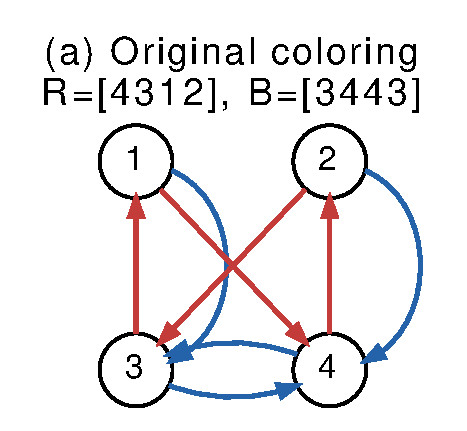
\includegraphics[width=\linewidth]{cc-original.eps}
\end{minipage}\hfill
\begin{minipage}[t]{0.48\textwidth}
\centering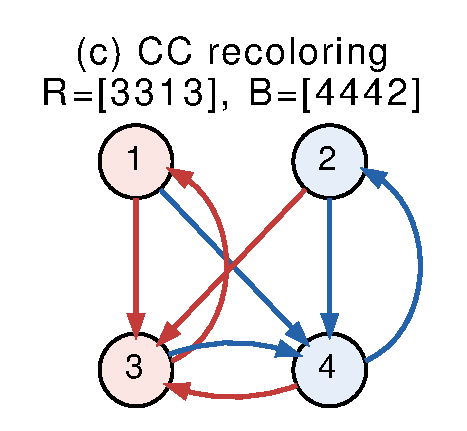
\includegraphics[width=\linewidth]{cc-cc.eps}
\end{minipage}

\medskip
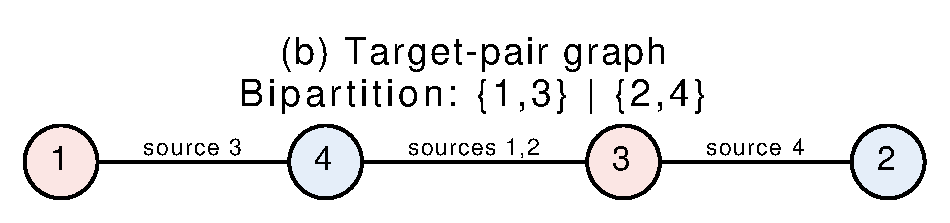
\includegraphics[width=0.92\textwidth]{cc-target.eps}
\caption{The four-state CC test. Top: (a) the original coloring and
(c) its CC recoloring, with red $R$-arrows and blue $B$-arrows.
Bottom: (b) the undirected target-pair graph; its edge $\{3,4\}$ comes
from both sources 1 and 2. Tinted vertices indicate the chosen red and
blue target types. The directed graph is unchanged; only the outgoing
colors at sources 1 and 4 are interchanged.}
\label{fig:cc-four-state-target-pair}
\end{figure}

\subsection{A test involving only matrix operations on $A$}
Define
\[
 L_A=\operatorname{diag}(A^{\mathsf T}\mathbf1)-A^{\mathsf T}A.
\]
\begin{proposition}\label{cc-exist:matrix-test}
For every coloring,
\[
 L_A=\Delta^{\mathsf T}\Delta.
\]
Consequently $L_A$ is positive semidefinite, $\dim\ker L_A=c$, and
\[
 \text{CC exists}\quad\Longleftrightarrow\quad
 \operatorname{nullity}A=\operatorname{nullity}L_A.
\]
\end{proposition}
\begin{proof}
Let $u=e_i$, $v=e_j$ be the two destination columns for one row.
That row contributes
\[
 \tfrac12(uu^{\mathsf T}+vv^{\mathsf T})
 -\tfrac14(u+v)(u+v)^{\mathsf T}
 =\tfrac14(u-v)(u-v)^{\mathsf T}
\]
to $L_A$. This is also its contribution to $\Delta^{\mathsf T}\Delta$,
regardless of which edge is red. The identity holds when $i=j$ as well.
Summing proves it, and the nullspace assertions follow from
$\ker(\Delta^{\mathsf T}\Delta)=\ker\Delta$ and
Theorem~\ref{cc-exist:equivalences}.
\end{proof}
The identity uses the equally weighted two-out hypothesis. It should not
be applied unchanged to an arbitrary stochastic matrix.

\subsection{Singularity is necessary but not sufficient}
An invertible $A$ rules out CC colorings. A singular $A$ need not admit one:
some components of $H_A$ may be bipartite while others are not.
For example, take
\[
 R=[24111],\qquad B=[35233].
\]
The directed graph is irreducible and aperiodic, while $H_A$ consists of
a triangle on $\{1,2,3\}$ and an edge on $\{4,5\}$. Therefore
\[
 \ker A=\operatorname{span}\{(0,0,0,1,-1)^{\mathsf T}\},
 \qquad \dim\ker\Delta=2.
\]
The transition matrix is singular, but no sign solution exists and there
is no CC coloring. If $H_A$ is connected, on the other hand, singularity
of $A$ is sufficient as well as necessary.

\subsection{Existence versus kernel rank}
These tests decide existence and construct all CC colorings; they do not
force synchronization. Our nine-state graph has two CC choices up to
color interchange, of kernel ranks three and one. Their associated RCCs
have ranks six and two. The six-state CC example $[312344],[666565]$
has a unique CC choice up to interchange; its RCC has partition
$(1234\mid56)$ and rank two.



\section{The matrix $\Delta$ annihilates only rank one kernels}  %III


Denote the all 1's (column) vector by $\bu$. 
We say that a word in $S$ has ``length $n$'' if it can be written as a product of $n$ $R$'s and $B$'s.


\begin{lemma} 		\label{lem:5.1}
Let the vector $\by$ satisfy $\Delta w\by=0$ for all words  $w \in S$.
Then $\by$ is a constant vector, i.e., a multiple of $\bu$.
\end{lemma}


\begin{proof}    Notice that  $\Dl\by=0$, implies that $R\by=B\by$. 
Thus,  $T\by = \frac{1}{2}(R+B)\by = R\by = B\by$.  
Inductively, assume that any word $w_n$  of length $n$ satisfies  $w_n\by=T^n\by$.  Now $Rw_n\by = Bw_n\by = Tw_n\by = T^{n+1}\by$  implies that any word $w_{n+1}$  of length $n+1$  satisfies  $w_{n+1}\by = T^{n+1}\by$.


Now let $e$ be an idempotent in the kernel, of length $l$. Then
\[
  e\by = T^l \by = e^2 \by = T^{2l} \by = \cdots = T^{nl} \by
\]
for all positive integers $n$. Letting  $n\to\i$ we get $\Om\by = c\bu$, where the constant  $c = \pi \cdot \by$.  
In other words, for every $i$ in the range of $e$, $y_i = c$. 
Since every $i$ occurs in the range of some idempotent in the kernel (this follows from strong connectivity), we get $\by = c\bu$.      
\qed
\end{proof}


\begin{corollary} 	\label{cor:5.1}
Let the vector $\by$ satisfy $\Dl T^n \by=0$  for all integer  $n \ge 0$.  
Then $\by$ is a constant vector, i.e., a multiple of $\bu$.
\end{corollary}


\begin{proof}    As above, from $\Dl \by = 0$, we get  $R\by = B\by = T\by$. 
Proceeding inductively as in the above proof $w_n\by = T^n\by$  for all words of length $n$ implies that $\Dl w_n \by = 0$  or 
\[
  Rw_n \by = Bw_n \by = Tw_n \by = T^{n+1} \by.
\]
Hence, $\Dl w\by = 0$ for all words $w$ and by the preceding Lemma, $\by$ is constant.
\qed
\end{proof}


\begin{corollary}   	\label{cor:5.2}
$\Dl k = 0$ for all $k \in K$  if and only if $K$  is rank one.
\end{corollary}


\begin{proof}     Suppose $\Dl k = 0$ for all $k \in K$.  
Let $e$ be an idempotent in $K$. 
Then for all words $w$,  $we \in K$, so that  $\Dl we = 0$,  for all $w$.  
By the Lemma, the columns of $e$ are constant vectors.  
Since any row has exactly one nonzero entry, one column is all ones and the rest are all zeros.  
The converse is immediate.
\qed
\end{proof}


\begin{corollary}   	\label{cor:5.3}
$\Dl e = 0$ for all idempotents in $K$ if and only if $K$ is rank one.
\end{corollary}


\begin{proof}     For any $k \in K$, since $K$ is completely simple and, therefore, a union of isomorphic groups, there is an idempotent such that  $k = ek$. 
Hence $\Dl k = \Dl ek = 0$ and by the previous Corollary, $K$ is rank one. 
\qed
\end{proof}




\section{Special rank one matrices in Vec($S$)}  %IV


In this section we will focus on the vector spaces generated by either the matrix semigroup or its kernel. 
Any rank-one matrix with identical rows in vec($S$) will be referred to as rank-one special, or ROSP.  
A ROSP in vec($K$) will be a KROSP.  
Note, that the ROSP’s form a vector space of dimension at most $n$.  
In general, we will identify a ROSP with its first row.  
Observe that if $M$ is any ROSP, then $MN$ is a ROSP for any matrix $N$ in vec($S$).
In addition, if $w$ is any word in $S$, $wM=M$.
That is, $M$ is a right zero for elements in $S$.


A \textit{range vector} is a vector consisting of 0's and 1's with 1's corresponding to the range of an idempotent $e$ in $K$, that is, a vector whose components indicate the non-zero columns of $e$. 
A range matrix is a KROSP whose rows equal some range vector.  
If there is no chance of confusion, for simplicity, we identify the range vector with its corresponding KROSP.


\begin{proposition}  \label{prop:5.2}
The vector space spanned by the KROSPs equals: 
\begin{enumerate}
\item[{\normalfont 1.}]  Span of $\{\Om w: w \in S \}$.
\item[{\normalfont 2.}]  Span of  $\{Mk: k \in K\}$, where $M$ is any ROSP in vec($S$) satisfying  $M\bu \not= 0$.
\item[{\normalfont 3.}]  Span of the range matrices.
\end{enumerate}
\end{proposition}


\begin{proof}    For \#1, first note that $\Om$ is an element of vec($K$), and therefore a KROSP (see the proof of Theorem [7] in \cite{BM}).  Since $K$ is an ideal, $kw \in K$, for any  $w \in S$.  
So $\Om w \in$ vec($K$) and hence a KROSP. 
Equality will follow from \#2.


For \#2, for  $k \in K$, $Mk \in$ vec($K$)  and so is a KROSP.   
If the set  $\{Mk : k \in K\}$ does not span the KROSPs, then there is a KROSP, $X$, with first row $\bx$ such that 
\[
  Mk\bx^t=0, \ \hbox{ for all } \ k \in K.
\]


Let  $M\bu = c\bu$, with  $c \not= 0$.  
Since $X$ itself is a KROSP, $cXX^t = MXX^t = 0$.  
So $X = 0$ and the result follows. 


For \#3, by the proof of Theorem 7 in \cite{BM}, $\pi k$ is a multiple of a range vector for every $k \in K$.  
So the result follows from \#2, taking  $M=\Om$. 
\qed
\end{proof}


The constant functions play a special role in any investigation of the road coloring problem. 
Let $C_i$ denote the matrix of the constant function $i$; that is for $C_i$, the $i$th  column is all ones.  
If $S$ contains the constants  $C_i$, they must be in $K$ due to minimality of the rank of the kernel.
Clearly, any element in the linear span of the constants  $C_i$, $i = i,\ldots,n$ is a KROSP.   
So the KROSPs have dimension $n$ if and only if vec($K$) contains the constants  $C_i$.  
In fact, we can say more.


\begin{proposition}  	\label{prop:5.3}
The KROSPs have dimension n if and only if the rank of the kernel is one.
\end{proposition}


\begin{proof}
One direction is immediate.  
For the other, assume that the KROSPs have dimension $n$. 
By the above, vec$(K)$ contains the constants $C_i$.


Now  $C_i = \sum\limits_{k \in K} \alpha_k k$.
Choose an idempotent $e \in K$.  
Then $eC_i e = \sum\limits_{k=K} \alpha_k eke$.  
Since $K$ is a completely simple semigroup (see \cite{CP}), then $eC_i e= C_j$  is in vec$(G)$ where $G = eKe$ is the subgroup for which $e$ is the local identity element (again \cite{CP}), and $ie=j$.


Suppose the rank of $K$ is $r$.  
Then $G$ is a group of block permutation matrices of rank $r$.  
In particular, the matrices of $G$ have $r$ nonzero columns.  
Notice $\Om C_j = C_j$.
On the other hand, $\Om C_j = \sum\limits_{k=K} \alpha_k \Om eke = C_j$.
But, as stated above, the proof of Theorem 7 in \cite{BM} shows that, for each $k \in K$, 
$\Om eke$ is a fixed ROSP whose rows are multiples of the range vector for the group $G$.  
Thus $C_j = \Om eke \sum\limits_{k=K} \alpha_k$ where $\Om eke$ is a ROSP with $r$ non-zero rows.  
But this is only possible if $r =1$. 
\qed
\end{proof}



\section{The Rank Condition}   %V


Recall that  $\pi$ denotes the invariant distribution, the row vector satisfying  $\pi T = \pi$, with  $\pi \cdot \bu = 1$.


\begin{definition}  \label{defn:5.2}
Let $d$ denote the rank of  $\Dl$.  
The \textit{rank condition} holds for $\Dl$ if the span of $\{\pi\Dl,\pi\Dl^2,\ldots,\pi\Dl^d\}$ is a $d$-dimensional space, in other words, these vectors span the range (row space) of  $\Dl$. 
\end{definition}


As a consequence of the rank condition, any vector $\by$ satisfying  $\Om\Dl^i\by=0$,  $1 \le i \le d$, satisfies $\Dl\by=0$ as well. 


Once again, the proof of Theorem 7 in \cite{BM} shows that $\pi k$ is a multiple of a range vector for every $k \in K$.  
Specifically, if $k$ is in $K$, then $\pi k$ is a multiple of the range vector corresponding to the nonzero columns of $k$, and that multiple depends only on the collection of non-zero columns, that is, the range of $k$.  
Observe that for any $k \in K$, $Rk$  and  $Bk$ are elements of $K$ with the same range.  
Hence, $\Om Rk=\Om Bk$, or $\Om\Dl k = 0$ for all  $k \in K$.


Assume the rank condition.  
Let $e$ be any idempotent in $K$. 
Let $w$ be any word in $S$.  
Then $Rwe$ and $Bwe$ are elements of $K$ with the same range.  
Hence, $\Om Rwe = \Om Bwe$ is a multiple of the range matrix corresponding to $e$. 
In other words, $\Om\Dl we=0$ for any $w$ in $S$. 
But then $\Om\Dl^ie=0$, for all $i \ge 0$,  since powers of $\Dl$ are in vec($S$). 
From the rank condition, we have $\Dl e=0$, for all idempotents  $e \in K$.  
By Corollary 3.4, $K$ is rank one.


We thus have the following


\begin{theorem}  	\label{thm:5.1}
The rank condition implies that the kernel is rank one.
\end{theorem}


The following Corollary is immediate, and is stated here only for completeness.


\begin{corollary}  	\label{cor:5.4} 
Let $G$ be a strongly connected, aperiodic graph.  
Suppose $G$ admits a coloring semigroup $S=\lrn{R,B}$ such that the rank condition holds for the difference matrix $\Dl= \frac{1}{2}(R-B)$ associated with the coloring.  
Then $S$ contains a synchronizing instruction.
\end{corollary}




%\hed{Coloring and recoloring}
\section{Coloring and recoloring}


The rank condition {\bf not} holding means that for every coloring $\phi$, there is a
polynomial $p_\phi$, of degree at most $d$, with $p_\phi(0)=0$,
such that $\Omega p_\phi(\phi\Dl)=0$.



Introduce variables $\vep_i$, $\vep_i^2=1$. Then generically
$$\phi=\hbox{diag}(\vep_1,\vep_2,\ldots,\vep_n)=
  \begin{pmatrix} 
	\vep_1&0&\cdots&0\cr 0&\vep_2&\cdots&0  \\ %\cr
          0&0&\ddots&0 \\		%\cr
          0&0&\cdots&\vep_n
   \end{pmatrix}	%\cr}
$$


We want the matrices $\{\Om\Delta,\,\Om\Delta^2,\,\ldots, \Om\Delta^d\}$ to be linearly
independent. Since these are all KROSPS, we form a matrix $H$ whose $i^{\rm th}$ row
is $\pi(\phi\Dl)^i$. Then the rank of $H$ is $d$ if and only if $\det HH^*\ne0$.
\bigskip


\begin{remark} Note that $\Om$ is always linearly independent of the $\Om\Dl^i$, just apply
to the all 1's vector. So if $d=n-1$, you can include $\pi$ as the first row of $H$ and get
an $n\times n$ matrix. Then you only need to check $\det H$.
\end{remark}



\subsection*{Procedure}

Initialize $\phi_0=\hbox{diag}(1,1,\ldots,1)$. 

\begin{enumerate}
\item[1.] Form $HH^*$.
\item[2.] Calculate $D(\phi)=\det HH^*$.
\item[3.] If $D(\phi_0)\ne0$, {\bf DONE} else continue.
\item[4.] Compute $\nabla_\vep D(\phi_0)$.
\item[5.] If any component of $\nabla_\vep D(\phi_0)$ is nonzero, recolor the corresponding vertex, {\bf DONE} else continue.
\item[6.] If all components of the gradient are zero, randomly pick a new $\phi_0$. Repeat from Step 3.
\end{enumerate}




% CC existence criterion added in the development manuscript.




%%%%%%%%%%%%%%%%%%%%%%%%%%%%%%%%%%%%%%%%%%%%%%%%%%%%%%%%%%
%%%
%%%  Semigroups and the Generalized Road Coloring Problem
%%%	Pgs 4-...
%%%%%%%%%%%%%%%%%%%%%%%%%%%%%%%%%%%%%%%%%%%%%%%%%%%%%%%%%%

\section{Main Result}
\label{sec:4.5}

In the remainder of the paper we will make the assumption that the graph $G$ is 2-out.  This assumption simply allows us to minimize notation.  
The argument can be extended to the $d$-out case.

\begin{theorem}		\label{thm:4.12}
	Let $A$ be the adjacency matrix of a strongly connected, 2-out digraph.
Suppose $\mathcal{S} = \lr r,b \rlr$, where $A = r+b$, is a minimal coloring semigroup
with kernel $K$.  Suppose $K = G \times Y$ is a right group, where rank $(K)=t$.  
Then $A$ is periodic of order $t$.
\end{theorem}

\begin{proof}	
Since $K$ is a right group, for any two idempotents $e_1,e_2$, both $e_1e_2=e_2$ and $e_2e_1 = e_1$.  
From this it follows that the partition of each function in $K$ is constant.  
That is, for all $k_1,k_2 \in K$,
\[
	\pi_{k_1} = \pi_{k_2} = \pi_K \hbox{ where}
\]
\[
	\pi_K = \{ Q_1,\ldots,Q_t \}
\]
and
\[
	Q_i = k^{-1}(v_i), \qquad v_i \in \hbox{Range(k)}, \quad i = 1,\ldots,t.
\]

Now $A$ is periodic of some order, say $p$.  
Thus, there is a partition of the vertices $\{ P_1,\ldots,P_p \}$ such that the graph can be written as in Figure \ref{fig:4.1}.
That is, an edge goes from vertex $v$ to $w$ iff $v \in P_i$ and $w \in P_{i+1}$ ($P_{p+1} \equiv P_1$).  
The partition $\pi_k$ is a refinement of $\{P_1,\ldots,P_p\}$.  
That is, for each $i$, $Q_i \subset P_j$ for some $j$.
This is clear, since if $k \in K$, $Q_ik = \{v\}$.  
Thus, there is a path connecting every vertex of $Q_i$ to vertex $v$.  
Thus, $Q_i \subset P_j$, for some $j$.

\begin{figure}[h]
\vbox to .6in{}
$$
	\special{eps:AMAT-Fig1.eps x=3in y=1.2in}
	\hbox to 3.2in{}
	%\figone
$$
\caption{The periodic partition of $A$.}
\label{fig:4.1}
\end{figure}

	
Next we show that both $r,b$ are 1 to 1 functions on the sets $\{Q_i: i = 1,\ldots,t\}$.

Suppose not.  
Then for some $v_1 \in Q_{i_1}$, $v_2 \in Q_{i_2}$,
%
\begin{align*}
	v_1r &\in Q_j \\
	v_2r &\in Q_j,
\end{align*}
%
but then if $k \in K$,
%
\begin{align*}
	v_1rk &\in Q_jk \\
	v_2rk &\in Q_jk,
\end{align*}
%
but since $k$ is an element of the kernel, $Q_jk$ is a single vertex.  
Since $v_1,v_2$ get mapped to the same vertex by $rk$ (also a member of the kernel), they must have started from the same element in the partition.  
Thus $Q_{i_1} = Q_{i_2}$ and $r$ is a one-to-one set function.  
Of course, the same argument is valid for $b$.

Notice that this shows that there must be exactly the same number of the $Q_i$'s in each of the periodic classes $P_1,\ldots,P_p$.  
This is true, since if there are  $n$  of the $Q_i$'s in $P_1$, $Q_1,\ldots,Q_n$, then each of these are mapped by $r$ into the $n$ $Q$-classes in $P_2$.  
Then $n$ $Q$-classes in $P_3$ are then images of these, etc. 
(See Figure \ref{fig:4.2}.) 
Observe, the above argument shows $p|t$. 
Also in Figure 2, we have renumbered the $Q$-classes, $Q_{ij}$, $i = 1,\ldots,p$, $j = 1,\ldots,n$ with 
$$
  (Q_{ij}) r \subset Q_{i+1,j}.
$$

\begin{figure}[t]
\vbox to .8in{}
$$
	\special{eps:AMAT-Fig2.eps x=3.4in y=1.2in}
	\hbox to 3.2in{}
	%\figtwo
$$
\caption{The graph of the function $r$.}
\label{fig:4.2}
\end{figure}


\noindent
Since we  have fixed the order of the $Q$-classes in $P_1$, the mapping from $P_p$ to $P_1$ is some arbitrary permutation, $\sigma$, that is
\[
	(Q_{p,1})r \subset Q_{1,\sigma(1)}
\]

Next we show that if $r=b$ as set functions, then $p=t$.

Suppose $r=b$.  
Choose $Q_{11}$ as the ``initial state'' and consider the cycle induced by powers of $r,b$
%
\begin{align*}
	Q_{11}r &\subset Q_{21} \quad \hbox{(also, } 
			Q_{11}b \subset Q_{21})	\\
	Q_{21}r &\subset Q_{31}, \quad \hbox{etc.}
\end{align*}
%
Suppose the above cycle is of length $\ell < t$.  
Then since $r,b$ are permutations (as set functions on the $Q$-classes) they are the product
of disjoint cycles.
In this case the graph would be disconnected, producing a contradiction. 
Thus, $\ell=t$. 

Clearly, if $c$ is any simple cycle within the graph, then $|c| = mt$ for some integer $m$.  
But since, if $c_1,\ldots,c_j$ is the set of all simple cycles, and
\[
	p = \gcd\{ |c_1|, |c_2|, \ldots, |c_j| \},
\]
then $t \le p$.  
Thus we have shown that if $r=b$, then the graph is periodic of order $t$.


Now suppose that $r \neq b$.  We must have the following.  (WLOG)

%        Picture 3
$$
\begin{picture}(300,27)(0,0)
    \thicklines
	\put(125,25){\vector(1,0){50}}
	\put(125,25){\vector(3,-2){50}}
	\put(125,-10){\vector(1,0){50}}
	\put(100,24){$Q_{11}$}
	\put(100,-11){$Q_{12}$}
	\put(185,23){$Q_{21}$}
	\put(185,-12.5){$Q_{22}$}
	\put(150,30){$r$}
	\put(160,7){$b$}
	\put(150,-20){$r$}
    \end{picture}
$$

\medskip
\noindent
Now recolor in the following way.

%        Picture 4
$$
\begin{picture}(300,27)(0,0)
    \thicklines
	\put(125,25){\vector(1,0){50}}
	\put(125,25){\vector(3,-2){50}}
	\put(125,-10){\vector(1,0){50}}
	\put(100,24){$Q_{11}$}
	\put(100,-11){$Q_{12}$}
	\put(185,23){$Q_{21}$}
	\put(185,-12.5){$Q_{22}$}
	\put(150,30){$b_2$}
	\put(160,7){$r_2$}
	\put(150,-20){$r_2$}
    \end{picture}
$$

\bigskip
\noindent
For all other edges, $r_2=r$, $b_2=b$.

Let $e = g_1 \cdot g_2 \cdot \ldots \cdot g_n$ be any idempotent in $K$, where $g_i = r$ or $b$.
Then for some $v_{11} \in Q_{11}$, $Q_{11} e = v_{11}$.

Form $g^1_1 \cdot g^1_2 \cdot \ldots \cdot g^1_n \in S_2 = \lr r_2,b_2 \rlr$ in the following way.
If $g_1 = r$, then $g^1_1 = b_2$ and if $g_1 = b$, then $g^1_1 = r_2$.
For $2 \le i \le n$,
\[
  g^1_i = \begin{cases}
	r_2 &\text{if } g_i = r \text{ and } Q_{11} g^1_1 
		\cdot \ldots \cdot g^1_{i-1} \not\in Q_{11}  \\
	b_2 &\text{if } g_i = b \text{ and } Q_{11} g^1_1 
		\cdot \ldots \cdot g^1_{i-1} \not\in Q_{11}  \\
	r_2 &\text{if } g_i = b \text{ and } Q_{11} g^1_1 
		\cdot \ldots \cdot g^1_{i-1} \in Q_{11}  \\
	b_2 &\text{if } g_i = r \text{ and } Q_{11} g^1_1 
		\cdot \ldots \cdot g^1_{i-1} \in Q_{11}  \\
  \end{cases}
\]
Thus, as in the second diagram above, change the color only after mapping into $Q_{11}$.
Then $Q_{11} g^1_1 \cdot g^1_2 \cdot \ldots \cdot g^1_n = v_{11}$ and we have collapsed the set $Q_{11}$ to a single vertex.

Now $Q_{12} g^1_1 \cdot g^1_2 \cdot \ldots \cdot g^1_n \subset Q_{1j}$ for some $j$.
Then $Q_{1j} e = v_{1j} \in Q_{1j}$.
As above, construct $g^2_1 \cdot \ldots \cdot g^2_n$ from $e$ by recoloring it if $Q_{1j}$ is mapped into $Q_{11}$.
Now $Q_{12} g^1_1 \cdot g^1_2 \cdot \ldots \cdot g^1_n \cdot g^2_1 \cdot \ldots \cdot g^2_n = v_{1j}$ and we have collapsed all of $Q_{12}$ to a single vertex.

Continue in this manner for each element $Q_{ij}$ of the partition, each time recoloring $e$ after mapping into $Q_{11}$, if this occurs.
Since $e$ collapses each element in the partition to a single vertex, at the end of this process we have constructed a function $h = g^1_1 \cdot \ldots \cdot g^1_n \cdot g^2_1 \cdot \ldots \cdot g^2_n \cdot \ldots \cdot g^t_1 \cdot \ldots \cdot g^t_n$ such that rank$(h) \le t$.

Suppose rank$(h) = t$.  
Then either each vertex in the range of $h$ is in a distinct $Q$ class or not.  
If there is a $Q$-class with more than one vertex from the range of $h$, then appending $e$ to $h$, once again recoloring as before, will collapse these vertices into a single vertex and reduce the rank to below $t$, thus contradicting minimality.  
If each $Q$-class has a single vertex in the range of $h$, appending first $r_2$ then $e$ (appropriately recolored) to $h$ will reduce the rank below $t$.

Thus, we have shown that $r$ must equal $b$ as set functions, and therefore the graph is periodic of order $t$.
\qed
\end{proof}


\chapter{Rank Tests, Cycles, and Potential Operators}
\label{organized:potential}
The target-pair graph controls the fixed ranks of $A$ and $\Delta$,
but does not determine the kernel rank or whether the positive powers
$\pi\Delta^i$ span the row space of $\Delta$. We now develop sufficient
ranked criteria. Section~\ref{app:four-state-recolorings} separates these
invariants from the changing ranks in a full recoloring run.
\paragraph{Notation in inherited proofs.}
The inherited source sections below write $N$ for the separation operator
$J-N$ of the current convention, and $N_0$ for the current collision
operator $N$. Their proofs must be read with this crosswalk until the
formula-by-formula notation revision is complete.


\section{Ranking}
\label{sec:6.6}

\begin{definition} 	\label{defn:6.1}
% BEGIN SUBJECT INDEX: defn:6.1
\index{cycle matrix}
\index{rank!matrix}
\index{rank!cycle matrix}
% END SUBJECT INDEX

Given a vector $v$ and matrix $T$, of rank $d$, define the span matrix, or, \textsl{cycle matrix\/}, 
$$
  \Sigma(v,T)=\begin{pmatrix}
  \hbox{---\quad} v T^{\hphantom 2} \hbox{\quad---} \cr 
  \hbox{---\quad}v T^2 \hbox{\quad---} \cr 
  \hbox{---\quad} \ \ \vdots^{\hphantom 2} \ \  \hbox{\quad---} \cr 
  \hbox{---\quad} v T^d \hbox{\quad---} \cr
  \end{pmatrix}
$$
with rows $\{vT,vT^2,\ldots,vT^d\}$.
\end{definition}

\begin{definition} 	\label{defn:6.2}
% BEGIN SUBJECT INDEX: defn:6.2
\index{ranked transformation}
\index{rank!ranked condition}
% END SUBJECT INDEX

Let $w$ be any word in $\cS$. 
Say that $w$ is \textsl{ranked\/} if the set $\{\pi w,\pi w^2,\ldots,\pi w^d\}$ is linearly independent, where $d={\rm rank}(w)$. 
\end{definition}

In other words, $w$ is ranked if $\rk \Sigma(\pi,w)=\rk w$.

\begin{theorem} 	\label{thm:6.1}
If $w$ is ranked, then the kernel, $\cK$, has rank one.
\end{theorem}

\begin{proof} Let $x_i=\pi w^i$ denote the $i^{\rm th}$ row of $\Sigma(\pi,w)$, the corresponding cycle matrix.
Let $e$ be any idempotent in $\cK$. Then by BM-F, we have 
$$
  x_i ee^*=\frac{1}{r}\,u
$$ 
Since every row of $w$ is a linear combination of the $x_i$, every row of $wee^*$ is constant. Since $w$ is a function,
a row of $wee^*$ is some row of $ee^*$. Since $\pi wee^*=(1/r)\,u$, $wee^*$ is not identically zero. So some row of
$ee^*$ is nonzero and constant. Hence that row consists of all 1's, which means that that vertex is in the same block of a partition of $\cK$
as every other vertex. In other words, $\cK$ is rank one.   \qed   
\end{proof}

Let $R$ have a single limiting cycle, $C$, of length $c$. Let $\eta_R$ be the idempotent for the kernel of the semigroup generated by $R$. Define the \textsl{closure\/} of $R$, $\R=\eta_RR$. So $\R$ has rank $c$.

Let $w=\R$ in the above Theorem.
Let $\Sigma'$ be the result of deleting zero columns from $\Sigma(\pi,\R)$.
The condition that $\R$ be ranked becomes that the determinant of $\Sigma'$ be nonzero. 
$\Sigma'$ has the form $CP$, where $C$ is a circulant and $P$ is a permutation. We thus find, after a suitable renumbering of the first row of $M'$, the required condition is 
that its {\it finite Fourier transform never vanishes\/}. 

\subsection{Ranking with $\boldsymbol\Delta$}
\label{sec:6.6.1}

Instead of working only with words from the semigroup, we can consider as well 
$ \Sigma(\pi,\Delta)$. We say $\Delta$ is ranked if $\rk \Sigma(\pi,\Delta)=\rk \Delta$.

\begin{theorem} 	\label{thm:6.2}
If $\Delta$ is ranked, then the kernel, $\cK$, has rank one. 
\end{theorem}

\begin{proof} 
Corollary \ref{cor:pideltan} says $\pi\Delta N=0$. In fact, Corollary \ref{cor:pideltann}
implies further that $\pi \Delta wN=0$ for all $w\in\cS$. Thus,
$\pi\Delta^i N=0$ for all $i\ge1$. If $\Delta$ is ranked, then $\Delta N=0$, and eq. \eqref{eq:N} reduces to
$$ 
  ANA^*=N
$$
Now Proposition \ref{propIRPER} yields $N=0$, i.e., $N_0=J$, which means the kernel is rank one. \qed
\end{proof}

\subsection{Ranking with $\mathbf{A+\vep\boldsymbol\Delta}$}
\label{sec:6.6.2}

Consider mixtures of $R$ and $B$ other than $50$-$50$. Taking $p,q\ge0$, $p+q=1$, we consider
$pR+qB$. Take $|\vep|\le1$ and set $p=(1+\vep)/2,q=(1-\vep)/2$. Then we set
$$
  A_\vep = pR+qB=A+\vep\Delta
$$
recovering $R$ when $\vep=1$ and $B$ when $\vep=-1$.  We say that $A_\vep$ is ranked if
$\rk \Sigma(\pi,A_\vep)=\rk A_\vep$. Note that $\vep=0$ gives back $A$, which cannot be ranked.
We have
 
\begin{theorem} 	\label{thm:6.3}
For $\vep\ne0$, if $A_\vep$ is ranked, then the kernel, $\cK$, has rank one.
\end{theorem}

\begin{proof} 
Calculate 
$$
  \pi A_\vep N=\pi(A+\vep\Delta)N=\pi N=r'u
$$
Similarly, expanding $A_\vep^i$, for $i>1$, apply $\pi$ on the left, using $\pi A=\pi$.
Except for $A^i$, we get terms of the form $\pi\Delta xN$ 
where $x$ is in the semigroup algebra. Hence, all terms vanish except
$\pi A^iN=\pi N=r'u$. If $A_\vep$ is ranked, then every row of $(A+\vep\Delta)N$ is constant.
I.e., $(A+\vep\Delta)N=bJ$, where $b$ is a diagonal matrix. Let $e_i$ be the standard basis row vector.
So the $i^{\rm th}$ row is
$$ 
  e_i(A+\vep\Delta)N=b_iu
$$
Applying this to $\dg \pi.$, using $N\dg\pi.=r'\dg u.$, yields $r'e_i\dg u.=b_i$. I.e., $b=r'I$ or
$$
  (A+\vep\Delta)N=r'J
$$
Writing $A_\vep$ in terms of $R$ and $B$, the $ij$ entry of $A_\vep N$ is
$$
  \underline{A_\vep N}_{\,ij}=pN_{iR,j}+qN_{iB,j}
$$
These are constant as $j$ varies. Taking $j=iR$, $j=iB$ and recalling the symmetry of $N$, we have
$$ 
  pN_{iR,iB}=qN_{iR,iB}
$$
Hence, if $p\ne q$,  $N_{iR,iB}=0$. So in row $iR$, the entries all vanish. By symmetry,
$N_{iB,iR}=0$ and the entries in row $iB$ vanish. But every vertex $i'$ is $iR$ or $iB$ for some $i$,
so $N$ vanishes identically, i.e., the kernel is rank one. \qed
\end{proof}



%%% Divisibility
\section{Divisibility}
\label{sec:6.7}
% BEGIN SUBJECT INDEX: sec:6.7
\index{divisibility!kernel rank and cycle length}
% END SUBJECT INDEX


Let $R$ have a single limiting cycle, $C$, of length $c$. Let $\R$ denote the closure of $R$.
The vector $u_c$ is $1\times c$ with all entries equal to 1. 

\begin{lemma} 		\label{lem:6.1}
The sum $\R+\R^2+\cdots+\R^c=\dg u.\chi_C$.
\end{lemma}

\begin{proof} Immediate since every vertex is either one step away from the cycle $C$ or is in the cycle so visits each point of the cycle exactly once. \qed
\end{proof}

\begin{theorem} 	\label{thm:6.4}
Let $r$ denote the rank of the kernel, $\cK$. Then $r|c$.
\end{theorem}

\begin{proof} Let $\Sigma=\Sigma(\pi,\R)$.
Let $e$ be any idempotent in $\cK$. Then by BM-F, we have 
$$
  \pi w ee^*=\frac{1}{r}\,u
$$ 
for any word in $\cS$. Hence,
$$
  u_c\Sigma ee^*=\,u_c(\frac{1}{r}\dg u_c.u)=\frac{c}{r}\,u
$$
On the other hand, by the Lemma,
$$
  u_c\Sigma ee^*=\pi\dg u.\chi_Cee^*=\chi_Cee^*
$$
which has integer entries. Hence the result. \qed
\end{proof}


\section{Applications}
\label{sec:6.8}

\subsection{Prime Cycle}
\label{sec:6.8.1}

If $c$, the length of a single limiting cycle for $R$, is prime, 
then the Fourier condition means that that the first row of $\Sigma(\pi,\R)'$ is not constant. 
Using BM-F, we know there is an aperiodic vertex. 
If not already synchronized, recoloring there guarantees that the probabilities on the cycle $C$ are nonconstant. 
Hence there is a kernel which is rank one.

\subsection{Friedman}
\label{sec:6.8.2}
% BEGIN SUBJECT INDEX: sec:6.8.2
\index{Friedman weight}
% END SUBJECT INDEX


Let $W$ denote the \textsl{Friedman weight\/}. I.e., rationalize $\pi$ to $\tilde\pi$ which has integer entries
with gcd equal to 1. These are the \textsl{weights\/}. The Friedman weight is the sum of those weights.
From BM-F it immediately follows that $r$, the rank of the kernel, divides $W$.
If $c$ and $W$ are relatively prime, then since $r$ divides both $c$ and $W$, the kernel $\cK$ has rank one.

\section{A potential operator and changes of letter probabilities}
\label{potential:section}
Let $R,B$ be stochastic matrices and suppose $A=(R+B)/2$ is irreducible
and aperiodic, with $\Omega=\mathbf1\pi$. Set
\[
 \Delta=(R-B)/2,\qquad Z=(I-A+\Omega)^{-1},\qquad V=\Delta Z.
\]
Since $\Delta\mathbf1=0$, we have $V\mathbf1=0$, $V\Omega=0$, and
\[
 V=\lim_{N\to\infty}\Delta\sum_{j=0}^N A^j.
\]
Indeed $\rho(A-\Omega)<1$ and $\Delta\Omega=0$. For an irreducible
periodic $A$, retain the algebraic definition and the Abel limit
$V=\lim_{t\uparrow1}\Delta(I-tA)^{-1}$, rather than this spectral-gap argument.

\begin{proposition}[Real-parameter invertibility]\label{potential:real-invertibility}
Under the standing hypotheses,
\[
 I-tV\text{ is invertible for every }t\in\mathbb R\text{ with }|t|<1.
\]
This is the replacement for Proposition 4.2 of \texttt{V-Operator.pdf};
no bound on the moduli of the nonreal eigenvalues of $V$ is asserted.
\end{proposition}
\begin{proof}
Put $A_t=A+t\Delta$. For real $|t|<1$, this is an irreducible stochastic
matrix, since its positive entries have the same support as those of $A$.
Suppose a row $x$ satisfies $x(I-tV)=0$. Since $V\mathbf1=0$,
we have $x\mathbf1=0$, hence $x\Omega=0$. Multiplying by
$Z^{-1}=I-A+\Omega$ gives
\[
 x(I-A+\Omega)=t x\Delta,
\]
so $xA_t=x$. The stationary row space of $A_t$ is one-dimensional;
its normalized stationary row has sum one. Therefore its only zero-sum
member is zero, and $x=0$. Thus $I-tV$ is invertible.
\end{proof}

\begin{theorem}\label{potential:interpolation}
For real $-1<\tau<1$, put $A_\tau=A+\tau\Delta$. Then
\[
 \Omega_\tau=\Omega(I-\tau V)^{-1},\qquad
 \pi_\tau=\pi(I-\tau V)^{-1}.
\]
At $\tau=1$, $I-V$ is invertible exactly when $R$ has a unique stationary
distribution. At $\tau=-1$, $I+V$ is invertible exactly when $B$ does.
In these cases the corresponding formula holds at the endpoint, using
the Cesaro projection of the endpoint matrix.
\end{theorem}
\begin{proof}
For interior real $\tau$, $A_\tau$ has the same support as $A$, hence a
unique stationary distribution. Also
\[
 (I-\tau V)Z^{-1}=I-A_\tau+\Omega.
\]
If a row $x$ annihilates the matrix on the right, multiplying by
$\mathbf1$ gives $x\mathbf1=0$, after which $xA_\tau=x$ forces $x=0$.
Thus the matrices are invertible. The stationary equations give
$\pi_\tau-\pi=\tau\pi_\tau V$, proving the formula.
At an endpoint, the same argument works precisely when the stationary
row space has dimension one. If it has higher dimension it contains a
nonzero zero-sum row, which gives a left nullvector of $I-A_\tau+\Omega$.
\end{proof}

\subsection{A necessary correction concerning the complex spectrum}
Invertibility for real $|\tau|<1$ does not imply $\rho(V)\le1$.
The spectral-radius assertion in Proposition 4.2 of the supplied
\texttt{V-Operator.pdf} must not be used as stated. For
\[
 R=[23451],\qquad B=[51234],
\]
$A$ is irreducible and aperiodic, while exact calculation gives
\[
 \det(\lambda I-V)=\frac{\lambda}{5}
 (5\lambda^4+10\lambda^2+1),\qquad
 \rho(V)=\cot(\pi/5)>1.
\]
The proof in the source uses stochastic uniqueness and therefore applies
to real parameters only. A Neumann series in $\tau V$ is justified locally
for $|\tau|\rho(V)<1$, not on the entire unit disk in general.
Nevertheless Theorem~\ref{potential:interpolation} holds throughout the
real interval. In particular,
\[
 \left.\frac{d^k\pi_\tau}{d\tau^k}\right|_{\tau=0}=k!\pi V^k.
\]

\subsection{Endpoint cycle measures and a wave operator}
If $R$ has a unique stationary distribution, define
\[
 U=(I+V)(I-V)^{-1}.
\]
Then
\[
 \Omega_B U=\Omega_R,\qquad U(I-R)=I-B.
\]
The endpoint identity $\Omega_B(I+V)=\Omega$ holds even when $B$ has
more than one recurrent class, so the first formula does not require
uniqueness for $B$.
For a deterministic generator with one limiting cycle $C$, its Cesaro
projection is $\Omega_R=\mathbf1\chi_C/|C|$. For any $k$ in the kernel,
$k\Omega_R=\Omega_R$, and the Cesaro averages of $kR^j$ belong to the
convex hull of the finite kernel. Thus $\Omega_R$ belongs to that convex
hull, hence to its linear span. The equal intersection counts
$|C\cap F|=|C|/r$ for kernel blocks $F$ connect this construction to the
cycle-divisibility results already developed in this chapter.

\subsection{An explicit partial-circulant potential}
For distinct indices $a,b$, take $R=M_a$, $B=M_b$ and use the unique
recurrent core. The potential has rank one and satisfies
\[
 V^2=\lambda V,\qquad \lambda=\frac{b-a}{a+b}.
\]
Consequently
\[
 (I-\tau V)^{-1}=I+\frac{\tau}{1-\tau\lambda}V,
 \qquad U=I+\frac{2}{1-\lambda}V.
\]
To see the scalar, write $V=e_1w$, so $V^2=w_1V$. The ladder formula gives
\[
 \pi_\tau(j)=
 \frac{(1+\tau)\mathbf1_{j\le a}+(1-\tau)\mathbf1_{j\le b}}
 {(1+\tau)a+(1-\tau)b}.
\]
On the other hand the rank-one inverse gives
$\pi_\tau(1)=\pi(1)/(1-\tau w_1)$. Comparing denominators yields
$w_1=(b-a)/(a+b)$. The formula is zero beyond $\max(a,b)$; transient
states are included in the operator but carry no stationary mass.
For periodic cores use the algebraic or Abel version of the potential.

\subsection{Adjugate and notation qualifications}
The adjugate identity in the source requires eigenvalue 1 to be
\emph{algebraically simple}, not merely to have a one-dimensional
eigenspace. Under that hypothesis, if $p(t)=\det(I-tX)$ and $P_X$ is the
spectral projection, then $\operatorname{adj}(I-X)=-p'(1)P_X$.
For a stochastic matrix with a unique stationary distribution the
hypothesis holds. The source's final $N_0=\mathbb E[EE^{\mathsf T}]$
is the collision operator denoted $N$ in our present convention.


\part{Higher representations and constructions}
\chapter{Tensor, Symmetric, and Zeon Hierarchies}
\label{organized:hierarchy}
\label{chapterseven}
\section{From particle configurations to the zeon quotient}
\label{hierarchy:collision-quotient}
Let $V$ have basis $e_1,\ldots,e_n$ over $\mathbb Q$. A deterministic
transformation $f$ sends $e_i$ to $e_{if}$ and acts on tensor powers by
\[
 (e_{i_1}\otimes\cdots\otimes e_{i_k})f^{\otimes k}
 =e_{i_1f}\otimes\cdots\otimes e_{i_kf}.
\]
This is simultaneous common-transformation motion of ordered particles.
Passing to $\operatorname{Sym}^k(V)$ forgets order but retains multiplicity:
repeated factors remain valid configurations.

\subsection{The invariant collision filtration}
Let $F_\ell$ be the span of degree-$k$ monomials with at most $\ell$
distinct occupied vertices. Deterministic transformations cannot increase
the number of distinct images, so
\[
 0\subseteq F_1\subseteq\cdots\subseteq F_k
 =\operatorname{Sym}^k(V)
\]
is an invariant filtration. The collision-free span itself need not be
invariant: distinct particles may collide. For $1\le k\le n$, the
quotient $F_k/F_{k-1}$ has basis the squarefree monomials $e_I$, indexed
by $k$-subsets, with action
\[
 e_I f^{\vee k}=\begin{cases}
 e_{If},&|If|=k,\\0,&|If|<k.
 \end{cases}
\]
This is the degree-$k$ zeon representation. Thus zeons isolate the
collision-free layer of the symmetric-power action rather than introduce
a different deterministic dynamics. Lost cardinality cannot be restored,
which proves $(fg)^{\vee k}=f^{\vee k}g^{\vee k}$.
An equivalent set-theoretic construction is the quotient of the module
on subsets of size at most $k$ by its submodule on subsets of size at most
$k-1$. This is not an exterior power: permutation signs are absent.

\subsection{Averages and limiting projections}
For deterministic generators $M_i$ chosen with probabilities $p_i$, put
\[
 A_k=\sum_i p_iM_i^{\vee k},\qquad
 \Omega_k=\lim_{m\to\infty}\frac1m\sum_{t=0}^{m-1}A_k^t.
\]
Each summand preserves the collision filtration before taking the quotient.
One must average these induced actions, not substitute the averaged
one-particle matrix into a symmetric-power formula. A general stochastic
linear map need not preserve the collision subspace of the symmetric
power. The independent-particle permanent construction is treated separately.

The basic observables remain visible in the full tensor construction.
Writing
\[
 \Phi(X)=\sum_i p_iM_iXM_i^{\mathsf T},\qquad
 \Psi(X)=\sum_i p_iM_i^{\mathsf T}XM_i,
\]
the limiting kernel measure gives
\[
 N=\lim_{m\to\infty}\frac1m\sum_{t=0}^{m-1}\Phi^t(I),\qquad
 M=\lim_{m\to\infty}\frac1m\sum_{t=0}^{m-1}\Psi^t(J).
\]
At zeon level two, $u_2=\Omega_2\mathbf1$ records survival of a distinct
pair, and its symmetric, zero-diagonal matrix realization is
\[
 \boxed{\operatorname{Mat}(u_2)=J-N.}
\]
The full projection $\Omega_2$ acts on pair space; $J-N$ is reconstructed
from its right field and is not that full projection. The $P_j,Q_i$
projections of Section~\ref{eproj:section} act on the original state space
and have yet another role. The following sections develop the higher
fields and their compatible inclusion maps within this framework.


\paragraph{Inherited operator convention.}
The inherited blocks in this chapter retain their source notation:
$N_0^{\mathrm{old}}=N$,
$N^{\mathrm{old}}=J-N$,
$M_0^{\mathrm{old}}=M$, and
$M^{\mathrm{old}}=M-\tau\omega$, where $\tau=\operatorname{tr}M$.
The superscripts in this crosswalk are editorial only; the inherited
formulas below still print the old symbols. A token-level mathematical
notation revision, not a global text substitution, remains necessary.
% use \chaptermark{}
% to alter or adjust the chapter heading in the running head


%%%%%%%%%%%%%%%%%%%%%%%%%%%%%%%%%%%%%%%%%%%%%%%%%%%%%%%%%%
%%%
%%%  The text below comes from (Feinsilver)
%%%  Trace Identities and Integration of Parts for Zeons
%%%
%%%%%%%%%%%%%%%%%%%%%%%%%%%%%%%%%%%%%%%%%%%%%%%%%%%%%%%%%%

\section{Zeon algebra and structure of the kernel}
\label{sec:7.1}

\subsection{Introduction}
\label{sec:7.1.1}

The notation $\diag{v}$ denotes the diagonal matrix with entries $v_i$ of the vector $\bf v$.

The \textsl{theta symbol\/} for pairs of single indices
$$
  \theta_{ij}=\begin{cases} 
	1, & \text{if } i<j\cr  
	0, & \text{otherwise} \end{cases}
$$

We indicate the component of a vector by underlining and then subscripting, e.g. $\underline{Tv}_{\,i}$
is the $i^{\rm th}$ component of the result of the matrix $T$ acting on the vector $v$.

$\V$ is the vector space isomorphic to $\BDQ^n$. Denote by ${\rm Sym}_n(\V)$ the space of
symmetric matrices acting on $\V$.

Denote by $\Z$ the algebra of \textsl{zeons}, generated by $n$ commuting variables $e_i$ such that
$e_i^2=0$, $1\le i \le n$. Then we identify $\V$ with the $\BDQ$-span of the zeons and generate
an algebra, $\Z$. The $k^{\rm th}$ zeon tensor power of $\V$ is denoted $\spow{\V}{k}$. 
Effectively $\spow{\V}{k}$ is the space of symmetric tensors with no repeated factors.
Elements of $\spow{\V}{k}$ are indexed by $k$-tuples of positive integers all distinct. 
I.e., the space has dimension $\binom{n}{k}$. We will denote multi-indices by 
roman capital letters $\rI=(i_1,i_2,\ldots,i_k)$, $\rJ$, $\rK$, etc. 
A linear operator $W$ on $\V$ extends to the operator $\spow{W}{k}$ acting on $\spow{\V}{k}$.
The \textsl{zeon Fock space\/}, 
$$ 
  {\mathcal F}=\BDQ\oplus (\bigoplus_{k\ge1}\spow{\V}{k})
$$
is finite dimensional, like the exterior algebra, and the \textsl{second quantization\/} of $W$ is the extension of 
$W$ to $\mathcal F$. Of course, one could work over a different field such as $\BDC$ for quantum mechanics with zeons.

The $\rI\rJ$ component of $\spow{W}{k}$ is the permanent of the corresponding submatrix of $W$ with
rows indexed by $\rI$ and columns by $\rJ$. For dimension 2, we will use indexes $ij$ instead
of $(i_1,i_2)$, as usual.

For given $n$, $X$, $Y$, etc., are vectors in $\spow{\V}{2}\approx\BDQ^{\binom{n}{2}}$.
The mapping \hfb ${\rm Mat}\colon\,\spow{\V}{2}\to {\rm Sym}_n(\V)$ is a linear embedding taking
the vector $X=(x_{ij})$ to the symmetric matrix $\hat X$ with off-diagonal components 
$\hat X_{ij}=x_{ij}=\hat X_{ji}$, for $i<j$ and zeros on the diagonal, $\hat X_{ii}=0$, $1\le i\le n$.
We will use the explicit notation ${\rm Mat}(X)$ as needed for clarity.

We equip $\spow{\V}{2}$ with the inner product 
$$
  \avg X,Y.=X_{\lambda\mu} Y_{\lambda\mu}=\tr \hat X\hat Y\ .
$$


%%% Basic Identities
\subsection{Basic Identities}
\label{sec:7.1.2}

Multiplying $X$ with $u$, we observe that
%
\begin{equation}\label{eqtrace1}
  X\dg u.=\frac12\,\tr \hat X J=u\dg  X.
\end{equation}
%
Observe also that if $D$ is diagonal, then $\tr D=\tr DJ$.

\begin{proposition}\label{propBR}   	\label{prop:6.6}
(\textsl{Basic Relations}) We have
\begin{enumerate}
\item[{\normalfont 1.}] $\Mat(X\spow{A}{2}) = \symm{A}{\hat X}-D^+$, where $D^+$ is a diagonal matrix satisfying $\vstrut\tr D^+=\tr \symm{A}{\hat X}$.

\item[{\normalfont 2.}] $\Mat(\spow{A}{2}\dg  X.) = \sym{A}{\hat X}-D^-$, where $D^-$ is a diagonal matrix satisfying $\vstrut\tr D^-=\tr \sym{A}{\hat X}$.

\item[{\normalfont 3.}] If $A$ and $X$ have nonnegative entries, then $D^+$ and $D^-$ have nonnegative entries. In particular, in that case,
vanishing trace for $D^{\pm}$ implies vanishing of the corresponding matrix.
\end{enumerate}
\end{proposition}

\begin{proof} The components of $X\spow{A}{2}$ are
%
\begin{eqnarray*}
\underline{X\spow{A}{2}}_{\,ij}  
  &=& \theta_{ij}\theta_{\lambda\mu}
	(x_{\lambda\mu}A_{\lambda i}A_{\mu j}
	+x_{\lambda\mu}A_{\mu i}A_{\lambda j}) \\
  &=& \theta_{ij} x_{\lambda\mu} A_{\lambda i}A_{\mu j}
	=\theta_{ij}\underline{\symm{A}{\hat X}}_{\,ij}
\end{eqnarray*}
%
noting that the diagonal terms of $\hat X$ vanish anyway. And $\symm{A}{\hat X}$ will be symmetric if $\hat X$ is.
Since the left-hand side has zero diagonal entries, we can remove the theta symbol and compensate by subtracting off
the diagonal, call it $D^+$. 
Taking traces yields \#1. And \#2 follows similarly.
\end{proof}

\begin{remark}   	\label{rem:7.1}
Observe that $D^+$ and $D^-$ may be explicitly given by
%
\begin{eqnarray*}
  D^+_{\,ii}  &=& x_{\lambda\mu}A_{\lambda i}A_{\mu i} \\
  D^-_{\,ii}  &=& x_{\lambda\mu}A_{i\lambda }A_{i\mu} 
\end{eqnarray*}
%
where for $D^+$ the $A$ elements are taken within a given column, while for $D^-$, the $A$ elements are in a given row.
\end{remark}

\begin{proposition}\label{propXX}  	\label{prop:7.2} %old 6.7
Let $X$ and $A$ be nonnegative. Then 
%
\begin{eqnarray*}
  \hat X = \symm{A}{\hat X}  &\Rightarrow&  X\spow{A}{2} = X\\
  \hat X = \sym{A}{\hat X}  &\Rightarrow&  \spow{A}{2}\dg  X. = \dg  X.
\end{eqnarray*}
%
\end{proposition}

\begin{proof} Start with
$$
  D^+= \symm{A}{\hat X}-\Mat(X\spow{A}{2})
$$
with $D^+$ vanishing if $\tr D^+=\tr \symm{A}{\hat X}$ vanishes.
If $\hat X = \symm{A}{\hat X}$, then since $\hat X$ has vanishing trace, $\tr \symm{A}{\hat X}=0$. 
Thus, $\tr D^+=0$ and $\hat X = \symm{A}{\hat X}=\Mat(X\spow{A}{2})$. 
The second implication follows similarly. 
\end{proof}

%%% Trace identities
\subsection{Trace Identities}
\label{sec:7.1.3}

Using equation (\ref{eqtrace1}), we will find some identities for these quantities.

\begin{proposition}\label{propTR}  \label{prop:7.3}
We have 
\begin{enumerate}
\item[{\normalfont 1.}] $\displaystyle X\spow{A}{2}\dg  u. = \half \,\tr (\hat X A(J-I)A^*)$ .

\item[{\normalfont 2.}] $\displaystyle u\spow{A}{2}\dg  X. = \half \,\tr (\hat X A^*(J-I)A)$ .

\item[{\normalfont 3.}] If $A$ is stochastic, then \ $X\spow{A}{2}\dg  u. = \half \,\tr (\hat X (J-AA^*))$.
\end{enumerate}
\end{proposition}

\begin{proof} We have, using equation (\ref{eqtrace1}) and Basic Relation 1,
%
\begin{eqnarray*}
  X\spow{A}{2}\dg  u.  
 &=& \half \,\tr \Mat(X\spow{A}{2})J\\
 &=& \half\,\tr (\symm{A}{\hat X}J-D^+J) \\
 &=& \half\,\tr (\symm{A}{\hat X}J-\symm{A}{\hat X})
 \end{eqnarray*}
%
and rearranging terms inside the trace yields \#1. 
Then \#3 follows since $A$ stochastic implies $AJ=J=JA^*$.
And \#2 follows similarly, using the second Basic Relation in the equation
$\displaystyle u\spow{A}{2}\dg  X. = \half \,\tr \Mat(\spow{A}{2}\dg  X.)J$.\qed
\end{proof}

Using  equation (\ref{eqtrace1}) directly for $X$, we have 
%
\begin{eqnarray}
X(I-\spow{A}{2})\dg  u.  &=&  \half \,\tr (\hat X (J-AJA^*+AA^*)) \label{eqbp1}\\
u(I-\spow{A}{2})\dg  X.  &=&  \half \,\tr (\hat X (J-A^*JA+A^*A))\label{eqbp2}
\end{eqnarray}
%


%%% stochastic case
\subsubsection{Stochastic case}
\label{sec:7.1.3.1}

For stochastic $A$, equation (\ref{eqbp1}) yields
\begin{equation}\label{eqparts}
X(I-\spow{A}{2})\dg  u. = \half \,\tr A^*\hat XA
\end{equation}

The above formula is ``integration-by-parts for zeons".

We denote an invariant distribution for $A$ by $\pi$, i.e. $\pi A=\pi=(p_1,\ldots,p_n)$.
We now have a converse result to Proposition 2. 

\begin{proposition}\label{propST}  	\label{prop:7.4}  %old 6.9
Let  $A$ be stochastic and $X$ nonnegative.
\begin{enumerate}
\item[{\normalfont 1.}] $X\spow{A}{2} = X \Rightarrow  \hat X = \symm{A}{\hat X}$.

\item[{\normalfont 2.}] If $A$ has a strictly positive invariant distribution, $\pi$, then \\
$\spow{A}{2}\dg  X. = \dg  X.   \Rightarrow  \hat X = \sym{A}{\hat X}\vstrut$.
\end{enumerate}
\end{proposition}

\begin{proof} If $X\spow{A}{2} = X$, then Proposition \ref{propBR}, eq. \eqref{eq:N}, reads
$$
  \hat X = \symm{A}{\hat X}-D^+
$$
Multiply by $\dg  u.$ on the right and by $u$ on the left, using  $A\dg  u.=\dg  u.$ and $uA^*=u$ to get
$$ 
  u\hat X\dg  u. =u\hat X\dg  u.-uD^+\dg  u.
$$
So $uD^+\dg  u.=0$ and taking traces yields $\tr(D^+J)=0$, thus $D^+=0$.

If $\spow{A}{2}\dg  X. = \dg  X. $, then Proposition \ref{propBR}, eq. \eqref{eq:M}, reads
$$
  \hat  X = \sym{A}{\hat X}-D^-
$$
Multiply by $\dg  \pi.$ on the right and by $\pi$ on the left, using $\pi A=\pi$ and $A^*\dg \pi.=\dg \pi.$ to get
$$
  \pi\hat X\dg  \pi. =\pi\hat X\dg  \pi.-\pi D^-\dg  \pi.
$$
So $\pi D^-\dg  \pi.=0$ and taking traces yields $\tr(D^-\dg  \pi.\pi)=0$. I.e., $\displaystyle \sum_i D^-_{ii}p_i^2=0$, so
$D^-=0$. \qed
\end{proof}

With $A$ stochastic, irreducible and aperiodic, $\displaystyle \lim_{n\to\infty}A^n = \Omega=\dg  u.\pi$, satisfying
$\Omega^2=\Omega=A\Omega=\Omega A$. Observe that
%
\begin{eqnarray*}
  \Omega\Omega^* &=& \dg  u.\pi\dg  \pi.u =(\sum p_i^2)\, J\\
  \Omega^*\Omega &=& \dg  \pi.u\dg  u.\pi = n\,\dg  \pi.\pi
\end{eqnarray*}
%
both of these having all positive entries.  Thus

\begin{proposition}\label{propIRPER} 	\label{prop:7.5}  %old 6.10 
Let $A$ be stochastic, irreducible and aperiodic. Then, for nonnegative $X$, either of 
$\hat X=\sym{A}{\hat X}$ or $\hat X=\symm{A}{\hat X}$ implies $X=0$.
\end{proposition}

\begin{proof} If $\hat X=\sym{A}{\hat X}$, then, inductively for positive integers $k$,
$$ 
  \hat X=A^k\hat X (A^*)^k
$$
Letting $k\to\infty$, we have $\hat X=\Omega \hat X \Omega^*$. Taking traces yields $\tr \hat X \Omega^*\Omega=0$. 
Since $\hat X$ is nonnegative and $\Omega^*\Omega$ is a matrix with positive entries, we have $X=0$. 
The proof for $\hat X=\symm{A}{\hat X}$ is similar.  \qed
\end{proof}

Now we have 

\begin{theorem}\label{thmIRPER}
Let $\spow{A}{2}\ne0$. 
Then\\ 
$A$ is aperiodic and irreducible if and only if $\det(I-\spow{A}{2})\ne 0$.
\end{theorem}

\begin{remark}		\label{rem:7.2}
Note that the hypothesis is saying that $A$ is not the identity matrix, i.e., that the chain moves at least one state to some other one.
\end{remark}

\begin{proof}
If $A$ is reducible, let $\{C_0,\ldots,C_{s-1}\}$ denote the closed classes partitioning the states.
Define $X$ by $x_{ij}=0$ if there is a $k$ such that $i,j\in C_k$, $1$ otherwise, i.e.,
$$ 
  X  = 1-\sum_k \chi_{C_k\times C_k}
$$
We will show that $\spow{A}{2}\dg  X.=\dg  X.$. 
\begin{description}
\item[Step 1.] First check that the diagonal vanishes, i.e., $A_{i\lambda}x_{\lambda\mu}A_{i\mu}=0$. 
By assumption, if $i\in C_k$, then
$\lambda,\mu\in C_k$. 
But then $x_{\lambda\mu}=0$. \\

\item[Step 2.] For $i\ne j$, $\underline{\spow{A}{2}\dg  X.}_{\,ij}=A_{i\lambda}x_{\lambda\mu}A_{j\mu}$. 
If $i\in C_k$, then the sum is over
$\lambda\in C_k$. If $j\in C_k$, then the sum is over $\mu\in C_k$ as well, $x_{\lambda\mu}=0$, and the result is zero.
If $j\in C_{k'}$, $k'\ne k$, then $x_{ij}=1$. 
Writing out the sum, we have
$$ 
  \sum_{l\in C_k, m\in C_{k'}} A_{il}x_{lm}A_{jm}
$$
For fixed $m$, $x_{lm}=1$, and the sum over $l\in C_k$ gives all choices that $i$ could map to, while for $l\notin C_k$, $A_{il}=0$, so 
$\displaystyle  \sum_{l\in C_k} A_{il}=1$. 
Similarly, summing over $m$ gives 1. 
Hence, we get $1$ in case $x_{ij}\ne0$ and
$0$ otherwise, as required. 
\end{description}

If $A$ is periodic, with period $p$, say, let $\{C_0,\ldots,C_{p-1}\}$ denote the classes partitioning the states such that 
$i\in C_k$ implies $iA\in C_{k+1}$, with indices modulo $p$.
Define $X$ by $x_{ij}=1$ if there exists $k$ such that $i\in C_k$ and $j\in C_{k+1}$, $0$ otherwise.  We check that 
$\spow{A}{2}\dg  X.=\dg  X.$.  The steps are similar to that for the case of reducibility:\\

Step 1. First check that the diagonal vanishes, i.e., $A_{i\lambda}x_{\lambda\mu}A_{i\mu}=0$. By periodicity, if $i\in C_{k-1}$, then
$\lambda\in C_k$ and hence $\mu\in C_{k+1}$ by definition of $X$. But then $A_{i\mu}$ vanishes since $\mu\in C_{k+1}$ requires
$i\in C_k$.\\

Step 2. For $i\ne j$, $\underline{\spow{A}{2}\dg  X.}_{\,ij}=A_{i\lambda}x_{\lambda\mu}A_{j\mu}$. If $i\in C_{k-1}$, then
$\lambda\in C_k$, $\mu\in C_{k+1}$ requires $j\in C_k$ so $x_{ij}\ne 0$. Now, writing out the sum, we have
$$ 
  \sum_{l\in C_k, m\in C_{k+1}} A_{il}x_{lm}A_{jm}
$$
For fixed $m$, $x_{lm}=1$, and the sum over $l$ gives all choices that $i$ could map to, i.e.,
$\displaystyle  \sum_{l\in C_k} A_{il}=1$. And summing over $m$, gives 1 as well. Hence, we get $1$ in case $x_{ij}\ne0$ and
$0$ otherwise, as required.\\

Suppose $A$ is aperiodic and irreducible.  By Perron-Frobenius the top nonnegative eigenvalue has a nonnegative eigenvector, $X$.
Proposition \ref{propST} says that a solution to $X\spow{A}{2} =X$ satisfies $\hat X=\symm{A}{\hat X}$. 
Then Proposition \ref{propIRPER} implies that $X=0$.
\end{proof}

%%% CSS

\subsection{Kernel structure}
\label{sec:7.1.4}

Let $\displaystyle A_2=\spow{A}{2}+\spow{\Delta}{2}=\half\,(\spow{R}{2}+\spow{B}{2})$.

For $\Delta$ we have, from Proposition \ref{propTR},
$$
  X\spow{\Delta}{2}\dg  u. 
  = \half \,\tr (\hat X (\Delta J\Delta^*-\Delta \Delta^*))
$$
which becomes
$$
  X\spow{\Delta}{2}\dg  u. = -\half \,\tr \Delta^*\hat X\Delta
$$
since $\Delta J=0$. And Proposition \ref{propTR}, \#2, yields
$$
  u\spow{\Delta}{2}\dg  X. 
	= \half \,\tr (\hat X (\Delta^*(J-I)\Delta)\ .
$$


\subsubsection{$\mathbf M$ and $\mathbf N$}
\label{7.1.4.1}

Note that $\Omega=\avg K.$, the average element of the kernel. As well, $\Omega=\beta_\lambda\rho(k_\lambda)$,
where $k_i$ runs through any row, so that each range is represented once.

Let $\omega$ be the diagonal matrix with $\pi$ on the diagonal, i.e. $\omega=\diag{\pi}$. 

\begin{proposition} \label{propKstarK} 	\label{prop:7.6}  %old 6.11
$\avg K^*K.=n\,\omega$.
\end{proposition}
\begin{proof}
For \#1, start by observing that $\diag{v}=\diag{\diag{v}{\rm \dg  u.}}$. Thus, since $k^*k$ is diagonal for every $k$, we check 
$\avg K^*K{\dg  u.}.=\avg K^*{\dg  u.}.=\Omega^*\dg  u.=n\,\dg  \pi.\ .$
\end{proof}

If  $\Omega_2$ is the limiting matrix of $A_2$, define $u_2=\Omega_2\dg  u.$ and $\pi_2=u\Omega_2$.
Then we have the following relations.

\begin{proposition}\label{propMN}  	\label{prop:7.7}  %old 6.12
For any $X$,
$$
  X\Omega_2\dg  u.=X\dg  u_2.=\avg X,u_2.
	=\half\,\tr \hat X\hat u_2 = \half\,\tr \hat XN
$$
where $N=\avg J-KK^*.$, taken over the kernel. \\
And
$$
  u\Omega_2\dg  X.=\pi_2\dg  X.
	=\avg \pi_2,X.=\half\,\tr \hat \pi_2\hat X 
	= \half\,\tr \hat X\tilde M
$$
where $\tilde M=\avg K^*(J-I)K.$, taken over the kernel.
\end{proposition}

\begin{proof} Using the homomorphism property of the map $\spow{\cdot}{2}$, we have $\Omega_2=\avg \spow{K}{2}.$ 
taken over the kernel. 
Thus, using Proposition \ref{propTR} for stochastic matrices, 
$$
  X\Omega_2\dg  u.=\avg X\spow{K}{2}{\dg  u.}.
	=\half\, \tr \avg \hat X(J-KK^*).= \half\,\tr \hat XN
$$
Similarly,
$$
  u\Omega_2\dg  X.=\avg u\spow{K}{2}{\dg  X.}.
	=\half\, \tr \avg \hat XK^*(J-I)K).
	= \half\,\tr \hat X\tilde M\ . \qed
$$ 
\end{proof}

Let $N_0=\avg KK^*.  = \avg EE^*.$, where $K$ denotes a random element of $\cK$, and $E$ denotes a random idempotent,
element of $\E(\cK)$. 
Define $N=J-N_0$. 
Since $\avg J.=J$, we set $u_2=\Omega_2\dg  u.$, satisfying $A_2u_2=u_2$, and identify $N$ as $\avg J-KK^*.=\Mat(u_2)$.
Note that $N=\alpha_\mu e_\mu e_\mu^*$ where the $e_i$ are (all of) the idempotents with a given range, i.e., they can be chosen as the idempotents from a single column in the kernel.

Let $M_0=\avg K^*JK.$. Define $\tau=\tr M_0$ and  $M=M_0-\tau\omega$.  Since $M$ and $\tilde M$ agree on off-diagonal 
elements, we set $\pi_2=u\Omega_2$, satisfying $\pi_2A_2=\pi_2$, and identify $M$ as $\Mat(\pi_2)$.

Note that $M_0$, $N_0$, $M$, $N$ as well as $J$ are all symmetric matrices.

Define the mappings, $F,G\colon {\rm Sym}_n(\V)\to{\rm Sym}_n(\V)$ by
$$ 
  F(Y)=\sym{A}{Y}+\sym{\Delta}{Y} \qquad\hbox{ and }\qquad
	G(Y)=\symm{A}{Y}+\symm{\Delta}{Y}\ .
$$
Note that
$$ 
  F(Y)=\half\,(\sym{R}{Y}+\sym{B}{Y}) \qquad\hbox{ and }\qquad
	G(Y)=\half\,(\symm{R}{Y}+\symm{B}{Y})\ .
$$
First, some observations

\begin{proposition}   	\label{prop:7.8}   %old 6.13
For any vector $v$, \rm $G(\diag{v}) = \diag{vA}$ .
\end{proposition}

\begin{proof} Let $Y=G(\diag{v})$. 
Then $2\,Y_{ij}=R_{\lambda i}v_{\lambda}R_{\lambda j}+B_{\lambda i}v_{\lambda}B_{\lambda j}$.
A term like $R_{li}$ means that $R$ maps $l$ to $i$. 
Since $R$ is a function, $l$ can only map to both $i$ and $j$ if $i=j$.
So $Y$ is diagonal. If $i=j$, then we get, using $R_{ij}^2=R_{ij}$, $B_{ij}^2=B_{ij}$,
$$
  2\,Y_{ii}=R_{\lambda i}v_{\lambda}+B_{\lambda i}v_{\lambda}
	=2\,v_\lambda A_{\lambda i}
$$
as required.
\end{proof}

For example, taking $v=u$, we see that 
$$
  G(I)=I \ \hbox{if and only if}\  A \ 
	\hbox{is doubly stochastic.}
$$

\begin{proposition}  	\label{prop:7.9}  %old 6.14
$F(J)=J$ and $G(\omega)=\omega$.
\end{proposition}

\begin{proof}
First, we have $F(J)=\sym{A}{J}+\sym{\Delta}{J}$, with $AJ=J=JA^*$ and $\Delta J=0$, this reduces to $J$.
Second, from the previous Proposition, we have $G(\omega)=G(\diag{\pi}))=\diag{\pi A}=\diag{\pi}=\omega$.
\end{proof}

Note that equation (\ref{eqparts}) applied to $R$ and $B$ and then averaged yields
%
\begin{equation} \label{eqPTS}
  X(I-A_2)\dg  u. =\half\,\tr G(\hat X)
\end{equation}
%

The next theorem shows the invariance of $N$ and $M$ under $F$ and $G$ respectively as well as the general relation between
fixed points of $A_2$ and fixed points of $F$ and $G$. 
Note that we are not restricting {\it a priori\/} to nonnegative solutions except in case 2 of the following theorem.

\begin{theorem}   \label{thm:7.2}  \hfill \\[-8pt]
\begin{enumerate}
\item[{\normalfont 1.}] $F(\hat X)=\hat X$ if and only if $A_2\dg  X.=\dg  X.$.

\item[{\normalfont 2.}] For nonnegative solutions $X$, $G(\hat X)=\hat X$ if and only if $XA_2=X$.
\end{enumerate}
\end{theorem}

\begin{proof}
First, from Proposition \ref{propBR}, applying the Basic Relations for $R$ and $B$ and averaging, we get
%
\begin{eqnarray}
\Mat(XA_2)  &=& G(\hat X)-\half\,(D_R^++D_B^+) \label{eqG}\\
\Mat(A_2\dg  X.)  &=&  F(\hat X)-\half\,(D_R^-+D_B^-)
\end{eqnarray}
%
where the subscripts on the $D$'s indicate the diagonals corresponding to $R$ and $B$ respectively.
Recalling the remark following Proposition \ref{propBR}, note that for $D_R^-$, say, we have terms like
$R_{i\lambda}x_{\lambda\mu}R_{i\mu}$. Since $R$ is a function, we must have $\lambda=\mu$, but then $x_{\lambda\mu}=0$.
In other words, $D_R^-$ and $D_B^-$ vanish so that, in fact,  $\Mat(A_2\dg  X.)  =  F(\hat X)$. And \#1 follows immediately.

For \#2,  if $G(\hat X)=\hat X$, then the trace of the diagonal terms in equation (\ref{eqG}) vanish, so under the assumption of
nonnegativity, they must vanish. And replacing $G(\hat X)$ by $\hat X$, we have $XA_2=X$.

Assume $XA_2=X$. Taking traces in equation \eqref{eqG}, the trace of the left-hand side vanishes and the trace of the diagonal
terms equals $\tr G(\hat X)$.  Now, use the integration-by-parts formula for $A_2$, equation \eqref{eqPTS}. The left-hand
side vanishes, hence $\tr G(\hat X)=0$, implying the vanishing of the terms $D_R^+$ and $D_B^+$ as well. Then equation
\eqref{eqG} reads $\Mat(X)=G(\hat X)$ as required. \qed
\end{proof}

From this Theorem we have \\

With $\displaystyle A_2=\spow{A}{2}+\spow{\Delta}{2}=\half(\spow{R}{2}+\spow{B}{2})$, 
we have $\Omega_2$ as the Ces\`aro limit of $A_2^k$.
Then with $u$ here denoting the all-ones vector of dimension $\binom{n}{2}$,
$u_2=\Omega_2\dg  u.$ and $\pi_2=u\Omega_2$. Then
\begin{enumerate}
\item[{\normalfont 1.}] $N=\avg J-KK^*.=\Mat(u_2)$ satisfies $\sym{A}{N}+\sym{\Delta}{N}=N$. It is a nonnegative solution with $\tr N=0$.
$N_0=\avg KK^*.$ and $J=\dg  u.u$ are also nonnegative solutions, with trace equal to $n$.\\

\item[{\normalfont 2.}] $M=\avg K^*(J-(\tau/n) I)K. =\Mat(\pi_2)$ satisfies $\symm{A}{M}+\symm{\Delta}{M}=M$. It is a nonnegative solution with $\tr M=0$.
$M_0=\avg K^*JK.$ and $\omega=\diag{\pi}$ are also nonnegative solutions, with trace equal to $\tau$ and $1$ respectively.
\end{enumerate}

Note that in Proposition \ref{propMN} we get $\tilde M=\avg K^*(J-I)K.$. However, $\tr \tilde M$ will not be zero. To cancel off the diagonal of $M_0$, we need to subtract off a multiple of $\omega$. 
From Proposition \ref{propKstarK}, we see that an appropriate multiple of $K^*K$ will work.


\subsubsection{Determinants and traces}
\label{sec:7.1.4.2}

Let $X=e_1\,{\rm adj}(I-\spow{A}{2})$ in equation \eqref{eqparts}. Since $X(I-\spow{A}{2})\dg  u.=\det(I-\spow{A}{2})$, we get
$$ 
  \det(I-\spow{A}{2})=\half\,\tr \symm{A}{\hat X}
$$

Similarly, let $X=e_1\,{\rm adj}(I-A_2)$ in equation \eqref{eqPTS}. 
We get
$$ 
  \det(I-A_2)=\half\,\tr G(\hat X)
	=\half\,\tr(\hat X(AA^*+ \Delta\Delta^*))
$$
Note that if $\det(I-A_2)=0$, then, if nonvanishing, $X=e_1\,{\rm adj}(I-A_2)$ will be a nontrivial solution to
$XA_2=X$. 
That is, if the solution space is one-dimensional, this is a multiple of $\pi_2$ and we scale to $\hat X=M$.
Then the vanishing of the trace will be equivalent to the vanishing of the determinant, i.e., the existence of solutions to $XA_2=X$.



%%%%%%%%%%%%%%%%%%%%%%%%%%%%%%%%%%%%%%%%%%%%%%%%%%%%%%%%%
%%%
%%%    The following text comes from (Feinsilver)
%%%    Kernel Hierarchy (PF-kernelHierarchy.tex)
%%%
%%%%%%%%%%%%%%%%%%%%%%%%%%%%%%%%%%%%%%%%%%%%%%%%%%%%%%%%%

\section{Levels}
\label{sec:7.2}  %old 6.11

Let $\pi$ be the invariant measure for $A=\half\,(R+B)$. Denote the components of 
$\pi$ by $(p_1,\ldots,p_n)$.

$r$ always denotes the rank of the kernel, $\cK$, of the semigroup $S=\avg R,B.$.\par
Indices, even though denoted as $\kappa$-tuples are {\it sets\/}, i.e., unordered, distinct elements,
denoted using capitals. [Note: read $\kappa$ as ``kay".] 

{\bf All vectors are row vectors. } Transposes will be denoted by superscript plus, so
that a typical column vector is $v^+$. We use roman type for the identity matrix.


For $1\le \kappa \le r$, let $R_1=R$, $R_\kappa$ denotes the mapping on $\kappa$-tuples induced
by $R$. 
I.e., for $\kappa$-tuples $\rI=(i_1,\ldots,i_\kappa)$, $\rJ=(j_1,\ldots,j_\kappa)$,
$$
  R_\kappa(\rI,\rJ)=\begin{cases} 
	1,& \text{ if } R \text{ maps the set of vertices } 
			\rI  \text{ to the set } \rJ \cr
        0, & \text{otherwise}\cr \end{cases}
$$

Similarly for $B_\kappa$. 
Then, we have 
$$ 
  A_\kappa=\half\,(R_\kappa+B_\kappa)\,,\qquad \Delta_\kappa
	=\half\,(R_\kappa-B_\kappa)
$$
For each $\kappa$, $R_\kappa$, $B_\kappa$, and $A_\kappa$ are substochastic matrices.

Note that $r\le \min(\rk(R),\rk(B))$ and is the maximal index $\kappa$ such that the semigroup $S_\kappa=\avg R_\kappa,B_\kappa.$ does not contain the zero matrix.

Generally, denoting by $w_\kappa$ the action of $w\in S$ induced on $\kappa$-tuples, we have, for any two words,
$w,w'\in S$, $(ww')_\kappa=w_\kappa w_\kappa'$, i.e., the map $w\to w_\kappa$ is a homomorphism of semigroups
$S\to S_\kappa$.


\section{Distributions}
\label{sec:7.3}
% BEGIN SUBJECT INDEX: sec:7.3
\index{Abel limit}
\index{limiting projection!higher representations}
% END SUBJECT INDEX
   %old 6.12

At level 1, we have left and right eigenvectors of $A$: $\pi_1=\pi$ and $u_1^+=u^+$, respectively.
All of the components of $u$ are equal to 1. And $\Omega=\Omega_1=u^+\pi$.\\
At every level $\kappa$, $1\le \kappa\le r$, we have an abel limit 
$$
  \Omega_\kappa=\lim_{s\uparrow1} (1-s)(I-sA_\kappa)^{-1}
$$
When $\pi_\kappa$ and $u_\kappa$ are unique, we have $\Omega_\kappa=u_\kappa^+\pi_\kappa$.

At level $r$, as at level 1, we have $\Omega_r=u_r^+\pi_r$.


\subsection{Interpretation}
\label{sec:7.3.1}

Start at level $r$. Then the nonzero entries of $\pi_r$ are in the columns corresponding to the ranges of the kernel, $\cK$. 
The nonzero entries of $u_r^+$ are in rows corresponding
to cross-sections of the partition classes of $\cK$. 
I.e., for each partition class, find all possible cross-sections weighted by one, take the total, then the corresponding entries of $u_r^+$ will be at least that. 
In particular, for a right group, all cross-sections appear with the same weight, which can be scaled to 1.

At each level, if unique, $\pi_\kappa$ and $u_\kappa$ give you the recurrent class and corresponding cross-sections.

To get a unique sequence of pairs $(\pi_\kappa,u_\kappa)$, construct them inductively from 
$(\pi_r,u_r)$ as consecutive marginals. 
Thus, for $\kappa<r$, let
$$ 
  \pi_\kappa(I)=\sum_{J\supset I}\pi_{\kappa+1}(J) 
$$
Note that in the sum each $J$ differs from $I$ by a single vertex. Starting from level $r$, we could thus set
$$
  \pi_\kappa(I)
	=\sum_{\substack{J\supset I\\ |J\setminus I|=r-\kappa}}\pi_r(J) 
$$
Thus, for each $\kappa$ there is a unique $\pi_\kappa$.\\
For $u$'s, proceed one step at a time:
$$ u_\kappa(I)=\sum_i p_i \,u_{\kappa+1}(I\cup \{i\}) $$
where the weights $p_i$ are the components of the invariant measure $\pi$.

With this construction, one recovers at level one, a multiple of $\pi_1=\pi$ and a
constant vector $u_1$, a multiple of $u$.



\section{Absorbing states}
\label{sec:7.4}   %old 6.13

Note that the kernel $\cK$ is rank one if and only if the semigroup $S_2=\avg R_2,B_2.$
contains zero. In this case, $\Omega_2$ is the zero matrix. More generally, $r$ is the maximum
level $\kappa$ such that $\Omega_\kappa\ne0$.

By introducing an absorbing state at each level, $R_\kappa$, $B_\kappa$, and $A_\kappa$, extended accordingly, are stochastic matrices as at level one.




% Checked extension from the new source notes.

\section{Inclusion operators and normalized compatible fields}
\label{organized:inclusion-fields}
Write $\alpha$ for the kernel partition distribution and $\beta$ for its
range distribution. A subset is split by a partition if its vertices lie
in different blocks. For $1\le\ell\le r$, define
\[
 u_\ell(I)=\Pr_\alpha\{I\text{ is split}\},\qquad
 \eta_\ell(I)=\binom r\ell^{-1}\Pr_\beta\{I\subseteq\mathcal R\}.
\]
Thus $\eta_\ell$ is a probability row, with $\eta_r=\beta$. For adjacent
levels the normalized range marginal is
\[
 \eta_\ell(I)=\frac1{\ell+1}
 \sum_{j\notin I}\eta_{\ell+1}(I\cup\{j\}).
\]
Indeed every $(\ell+1)$-set contributes to exactly $\ell+1$ of its
$\ell$-subsets. Equivalently, count the $r-\ell$ extensions inside a
fixed range and use the binomial coefficients.

Equipartition gives the exact right-field normalization
\[
 u_\ell(I)=\frac r{r-\ell}
 \sum_{j\notin I}\pi_j u_{\ell+1}(I\cup\{j\}),\qquad\ell<r.
\]
For a fixed kernel partition, an already split $I$ occupies $\ell$ blocks;
the union of the unoccupied blocks has stationary mass $(r-\ell)/r$.
If $I$ is not split, no extension is split. Average this identity over
$\alpha$ to obtain the formula.

The incidence matrix $E_{\ell+1,\ell}(J,I)=\mathbf1_{I\subset J}$
expresses the first recurrence in operator form. The common-letter lift
maps each kernel range injectively to another range, so its top stationary
range law descends to stationary $\eta_\ell$ at every level.
The right field is $u_\ell=\Omega_\ell\mathbf1$, with the Abel projection
$\Omega_\ell$. One must not infer that every intermediate projection has
rank one, or identify a normalized row $\mathbf1^{\mathsf T}\Omega_\ell$
with the chosen top-range marginal without an argument.
The full inclusion-compatibility identities and their proofs have their
primary source in \texttt{kernelHierarchy.tex}; this section fixes the
normalizations used in the organized edition.


\chapter{Permanental Markov Chains}
\label{organized:permanents}
\section{Permanents as killed independent-particle transitions}
\label{organized:permanent-core}
For a stochastic matrix $P$ and $k$-subsets $I,J$, define
\[
 Q_k(I,J)=\operatorname{per}P[I,J].
\]
This is the probability that $k$ independently moving labeled particles,
initially at distinct states $I$, occupy the distinct unordered states $J$
after one step. The permanent sums the assignments of labels to $J$.
The matrix is substochastic: the missing row mass is the probability of
a collision. A cemetery state makes it stochastic; repeated powers track
survival without collisions at every intermediate step.
In general $Q_k^t\ne(P^t)^{\vee k}$, since the latter permits intermediate
collisions followed by separation. General permanental lifts are not
multiplicative. They are multiplicative for deterministic transformations.

\section{A positivity hypothesis in the converse}
Suppose $P$ has a strictly positive stationary distribution. Then
\begin{theorem}\label{organized:permanent-criterion}
The following are equivalent: $P$ is irreducible and aperiodic;
$\rho(Q_2)<1$; and $\det(I-Q_2)\ne0$.
\end{theorem}
\begin{proof}
If $P$ is primitive, choose $t$ with every entry of $P^t$ positive.
For every distinct starting pair the independent particles have a
uniformly positive probability of meeting at time $t$. The probability
of surviving without any collision through time $t$ is therefore
uniformly less than one. Hence $\|Q_2^t\|_\infty<1$ and $\rho(Q_2)<1$.
If $P$ is reducible, strict positivity of a stationary row excludes
transient states. There are then at least two closed classes; a particle
in each cannot collide. If $P$ is irreducible but periodic, two particles
in different cyclic classes also cannot collide. In either case the
finite killed chain has a nonempty closed stochastic class and $Q_2$
has eigenvalue one. Finally a nonnegative substochastic matrix has
spectral radius at most one, and if it equals one, one itself is an
eigenvalue. This proves the determinant equivalence.
\end{proof}
Without strict positivity the converse fails. For example
$P=\left(\begin{smallmatrix}1&0\\1&0\end{smallmatrix}\right)$ has
$Q_2=0$ but is not irreducible. Thus uniqueness of a stationary measure
alone is not the hypothesis of this theorem.

\section{Independent versus common-letter motion}
For $P=\sum_i p_iM_i$, distinguish
\[
 P^{\vee k}\quad\text{from}\quad\sum_i p_iM_i^{\vee k}.
\]
The first uses independent choices and kills collisions; the second uses
one common random transformation. They agree for PtC because every
generator differs only in row 1 and a submatrix contains that row at most
once. The detailed proof is in the laboratory chapter. This equality is
special, not a general averaging rule.


\chapter{Coupled Semigroups and Opposite Letters}
\label{organized:couplings}
\section{Opposite-letter tensor coupling and its kernel}
\label{opp-tensor:section}
% BEGIN SUBJECT INDEX: opp-tensor:section
\index{opposite-letter dynamics}
\index{tensor coupling}
% END SUBJECT INDEX

Let $S=\langle R,B\rangle$ be a finite transformation semigroup, with
kernel $K$ of rank $r$. For a word $w$, let $\bar w$ exchange every $R$
and $B$. Define
\[
 T_-=\langle(R,B),(B,R)\rangle\subseteq S\times S.
\]
Its action on ordered pairs is represented by $R\otimes B$ and
$B\otimes R$, and a word gives $(w,\bar w)$.

\begin{theorem}\label{opp-tensor:kernel}
The kernel of the opposite-letter semigroup is
\[
 K_-=T_-\cap(K\times K),
\]
and every element of $K_-$ has transformation rank $r^2$ on $X\times X$.
Both coordinate projections $K_-\to K$ are surjective.
\end{theorem}
\begin{proof}
The rank of $(f,g)$ on $X\times X$ is
$\operatorname{rank}(f)\operatorname{rank}(g)\ge r^2$.
Choose a word $u\in K$. The word $u\bar u$ gives the pair
$(u\bar u,\bar u u)$; both coordinates lie in $K$ by the ideal property.
Thus minimum rank is $r^2$, attained exactly when both coordinates lie
in $K$. The minimum-rank ideal of a finite transformation semigroup is
its kernel, proving the formula. Each coordinate projection of $T_-$
is onto $S$. Its image of $K_-$ is a nonempty ideal of $S$ contained in
$K$, and hence equals $K$.
\end{proof}
The product fibers are $F\times G$ and the product ranges are
$A\times B$, but only the pairs compatible with complementary words occur.
Local groups are subdirect products of the two corresponding local groups:
restriction to an idempotent cell is a subgroup of their product, and
sandwiching preimages by that idempotent proves surjectivity on each factor.

\subsection{The original kernel alone is insufficient}
Letter exchange need not define a map on $S$: equality $w=v$ need not
imply $\bar w=\bar v$. If it does define an automorphism $\theta$, then
$T_-$ is its graph and $K_-=\{(k,\theta(k)):k\in K\}$.
In general the required extra information is complementary-word compatibility.
For a concrete counterexample, the pairs
\[
 [312344],[666565]\qquad\text{and}\qquad [112345],[612345]
\]
have the same concrete base kernel, all six constant maps, but their
opposite-letter kernels have respectively 16 and 31 elements.
For the second pair, $R^5B^5$ is a reset word on the product state space;
its target is $(2,1)$ and its orbit has 31 points. For the first pair,
$R^2B$ resets to $(6,4)$, whose orbit has 16 points. Once one constant
product map is obtained, its orbit gives every constant product map,
so these finite orbit counts determine the two kernels.

\subsection{The running examples}
Exact enumeration gives
\[
\begin{array}{c|r|r|r|r|r|r}
\text{example}&|T_-|&|K_-|&\text{rank}&\text{partitions}&\text{ranges}&|G_-|\\
\hline
4\text{ states}&44&36&4&3&3&4\\
6\text{ states}&44&16&1&1&16&1\\
9\text{ states}&300&288&9&4&4&18
\end{array}
\]
The examples are the previously studied pairs $[4312],[3443]$,
$[312344],[666565]$, and $[444777111],[295838562]$.
In the nine-state example the local group is
\[
 \{(\sigma,\eta)\in S_3\times S_3:
       \operatorname{sgn}\sigma=\operatorname{sgn}\eta\}.
\]
Enumeration in an idempotent cell produces all 18 equal-parity pairs.
Thus it is not the full product of the original local groups.
For six states the kernel constants have targets precisely in
\[
 (\{1,2,3,4\}\times\{5,6\})\ \cup\
 (\{5,6\}\times\{1,2,3,4\}),
\]
the opposite-type sector of the CC coloring.

\subsection{Same-letter and opposite-letter chains}
For $A=(R+B)/2$ and $\Delta=(R-B)/2$, put
\[
 P_+=\tfrac12(R\otimes R+B\otimes B)
     =A\otimes A+\Delta\otimes\Delta,
\]
\[
 P_-=\tfrac12(R\otimes B+B\otimes R)
     =A\otimes A-\Delta\otimes\Delta.
\]
Use Cesaro or Abel limits unless convergence of ordinary powers is
proved. The limiting kernel measure of $T_-$ need not be the product
of the two original kernel measures; both word and probability correlations matter.

If $A$ is primitive, the midpoint $Q=A\otimes A$ is primitive with
stationary projection $\Omega\otimes\Omega$. The preceding potential
construction applies with
\[
 D=\Delta\otimes\Delta,\qquad
 V_{\mathrm{pair}}=D(I-Q+\Omega\otimes\Omega)^{-1}.
\]
It interpolates $Q+\tau D$ between $P_-$ and $P_+$.
Invertibility of $I\mp V_{\mathrm{pair}}$ detects uniqueness of the
stationary distribution at the respective endpoints. For $P_+$,
uniqueness is equivalent to synchronization: the diagonal is a closed
irreducible class; if it is the only recurrent class every pair can be
merged, hence successive pair mergers synchronize the entire set.
Conversely a reset word makes all off-diagonal states transient.

For a CC target-sign column $s$, we have $As=0$, $\Delta s=\mathbf1$,
and $\pi s=0$. Therefore
\[
 Q(s\otimes s)=0,\qquad D(s\otimes s)=\mathbf1.
\]
If $\mu_\tau$ is the stationary row of $Q+\tau D$, then
\[
 \mu_\tau(s\otimes s)=\tau.
\]
At the endpoints this is the same-type sector for $P_+$ and the
opposite-type sector for $P_-$. This is a direct connection between
the potential operator, the tensor hierarchy, and canonical colorings.

\subsection{A partial-circulant consequence}
Let the base generators be $M_a,M_b$, with $d=\gcd(a,b)$. Their kernel
has one partition, the residue classes modulo $d$, and local group $C_d$.
The opposite-letter kernel also has one partition, namely the products
of those residue classes. It is therefore a right group, of transformation
rank $d^2$. Its local group is still $C_d$, rather than $C_d\times C_d$.
Indeed each letter decreases both coordinates by one modulo $d$, so
both coordinate phases of every kernel pair agree. In an idempotent cell
the local group is contained in the diagonal $C_d$ and projects onto it,
hence equals it. The remaining problem is to characterize the compatible
pairs of ranges, not to determine the local group.
The relative residue $x-y\pmod d$ is preserved, explaining why the local
group need not act transitively on all $d^2$ points of a product range.
The example $M_1,M_6$ already shows nontrivial range compatibility when $d=1$.


\chapter{Graph Lifts and the Double Construction}
\label{organized:lifts}
\section{The edge-state lift}
\label{organized:double-core}
Order the $2n$ edge states by the red outgoing edge from each vertex,
then the blue one; parallel edges remain distinct labeled edge states.
The induced transformations and their average are
\[
 \widehat R=\begin{pmatrix}R&0\\B&0\end{pmatrix},\quad
 \widehat B=\begin{pmatrix}0&R\\0&B\end{pmatrix},\quad
 \widehat A=\tfrac12\begin{pmatrix}R&R\\B&B\end{pmatrix}.
\]
If $\pi A=\pi$, then
\[
 \widehat\pi=(\pi R/2,\pi B/2).
\]
Multiplication verifies the identity, since $\pi R+\pi B=2\pi$.
In general this is not $(\pi/2,\pi/2)$.
Writing $U=\tfrac12[R;B]$ and $W=[I,I]$ gives $\widehat A=UW$,
$A=WU$, so
\[
 \det(\lambda I_{2n}-\widehat A)=\lambda^n\det(\lambda I_n-A).
\]

\section{Kernel rank and kernel elements under the lift}
Assume every vertex has an incoming edge, as in the irreducible case.
Let $H=[R;B]$ be the head map, and $J_R=[I,0]$, $J_B=[0,I]$ the two
edge injections. Then $\widehat L=HJ_L$ and $J_LH=L$.
For a nonempty word $w=L_1\cdots L_t$,
\[
 \widehat w=H(L_1\cdots L_{t-1})J_{L_t}.
\]
The head map is onto and each $J_L$ is injective, so the rank is the
rank of the prefix. If the base kernel has rank $r$, the lifted kernel
therefore has rank $r$ and is precisely
\[
 \widehat K=\{HkJ_R,HkJ_B:k\in K\}.
\]
If a prefix is empty its rank is $n$; it contributes to the kernel only
when $r=n$, in which case the base semigroup is a group containing the
identity. The two last-color ranges are disjoint and $H$ is onto, so
these representations are distinct and $|\widehat K|=2|K|$.
Kernel partitions pull back through $H$; kernel ranges are the two edge
copies of the base ranges. Transport of all hierarchy fields is a
further question, not an automatic identification of stationary laws.

\section{A systematic source of CC examples}
Every outgoing pair at a lifted source consists of edge vertices $i$
and $i+n$, where $i$ is its head. Since every head occurs, the auxiliary
target-pair graph is exactly a matching of $n$ pairs. Thus the double is
CC and has $2^n$ labeled CC choices. The displayed lift is one such
choice, with disjoint red and blue ranges.
Graph doubling preserves the kernel rank in this coloring; canonical
recoloring of that CC coloring doubles it. These are different operations.
This distinction is essential when comparing the lift with the CC
rank-doubling theorem.


\part{Synthesis}
\chapter{Lie Methods and Lie Constants}
\label{organized:lie}
Separate the proved solvability/right-group implication from the Lie-constant converse, which remains unproved in this project.





%%%%%%%%%%%%%%%%%%%%%%%%%%%%%%%%%%%%%%%%%%%%%%%%%%%%%%%%%%
%%%
%%%  Completely Simple Semigroups, Lie Algebras, 
%%%   and the Road Coloring Problem 
%%%	
%%%%%%%%%%%%%%%%%%%%%%%%%%%%%%%%%%%%%%%%%%%%%%%%%%%%%%%%%%


\section{Completely Simple Semigroups, Lie Algebras, 
  and the Road Coloring Problem }
\label{sec:4.8}

Studying the dynamics inherent in state-transition diagrams, either in the stochastic setting as Markov chains or in deterministic models as automata, continues to be a rich source of interesting mathematics and applications. 
Even for finite state systems, fascinating unsolved problems exist.
\^Cern\'y's conjecture concerning the length of a synchronizing instruction for deterministic automata is one such example. 
Another open problem in this area is referred to as the ``road coloring problem'' and was the initial motivation for this work. 
The road coloring problem appeared in published form for the first time in a paper by Adler, Goodwyn, and Weiss \cite{AGW} and can be stated very simply:  Suppose you are given a strongly connected directed graph (or state-transition diagram).  
Is there a way to label the edges so that a synchronizing  instruction exists? 
A precise definition of synchronizing instruction will be provided below. 
In \cite{AGW},  it was shown that aperiodicity was necessary for such an instruction to exist. 
The road coloring problem conjectures that aperiodicity is a sufficient condition as well. 

\subsection{Background} 
\label{sec:4.8.1}

A finite automaton consists of a finite set $V$ of states, a finite set of inputs $A$, and a state transition function $\dl :V\times A \to V$.
We can associate with each $a \in A$ a corresponding transformation $R_a: V \to V$ defined by $R_a(v) = \dl(v,a)$, which we write compactly as $va$.
The semigroup $S$ generated under composition by $\{R_a: a \in A\}$ is called the semigroup of the automaton.
Given any automaton, one obtains a labelled digraph by taking the vertices of the graph to be the set of states $V$ and for each $(v,a) \in V \times A$ defining a directed edge from $v$ to $va$ with label $a$.  
Note that the constructed directed graph has \textit{uniform outdegree}, i.e., each vertex of $V$ has the same number of edges leading from it.

If one considers an unlabelled digraph $G = (V,\E)$ of uniform outdegree $d$, then any labelling of the edges with members of $A$, where $|A| = d$, such that each edge issuing from any given vertex has a distinct label is called a \textit{coloring} of the digraph.
Any such coloring uniquely determines an automaton $\dl: V \times A \to V$, where $R_a(v) = va$ is the terminal point of the directed edge with initial point $v$ and label $a$.  
We henceforth assume that digraphs have uniform outdegree, identifying the coloring with the set $\C = \{R_a: a \in A\}$, and we refer to the semigroup $S = \lr \C \rlr$, generated by $\C$, as the \textit{coloring semigroup} for the given labelling.

\begin{definition}   \label{defn:4.6}
Let $S$ be a coloring semigroup of a digraph $G = (V,\E)$.
The \textit{rank} of $s \in S$ is the cardinality $|Vs|$ of the image of $s$.
Any finite transformation semigroup $S$ has a minimal ideal or \textit{kernel}, which consists of the elments of minimal rank (see \cite{H}).
This common minimal rank is called the \textit{rank of the kernel}.
\end{definition}

A \textit{synchronizing instruction} for an edge-labelled digraph is thus any transformation of rank one.
The road coloring problem can now be stated in the following way.

\runinhead{Road Coloring Conjecture.}
\textit{Let $G = (V,\E)$ be a $d$-out, strongly connected digraph.
Let $\{S_i\}$ be the set of all coloring semigroups.  
If $G$ is aperiodic, then for some $i$, $S_i$ contains a synchronizing instruction.} \\

The notion of period used here is the standard one from Markov chain theory, where for any vertex $v$ in a directed graph, $\hbox{per}(v) - \gcd\{|c_1|, \ldots , |c_n|\}$ where $c_1, \ldots , c_n$ are the simple cycles containing $v$.
The assumption of strong connectivity ensures that all vertices have the same period.

\runinhead{Notation.}  We use rank and trace to denote the rank and trace respectively of a matrix.
For a function, rank and trace refer to its representing matrix.

\subsection{Semigroups and kernels}
\label{sec:4.8.2}

Let $S$ be a coloring semigroup of a strongly connected digraph with kernel $K$.
Let $E(S)$ be the set of idempotents of $S$. 
Impose on $E(S)$ the order $e \le f$ iff $ef = fe = e$.
Form the Rees product $x \times G \times Y$ of $K$ in the usual manner choosing an idempotent, $e_0$, minimal with respect to this order and letting
\[
  x = E(Ke_0), \quad G = e_0Ke_0, \quad Y = E(e_0K)
\]
with product
\[
  (x_1,g_1,y_1)(x_2,g_2,y_2) := (x_1,g_1(y_1x_2)g_2,y_2)\,.
\]
Notice that $y_1x_2 \in G$.
The sandwich function
\[
  \phi: Y \times X \to G, \qquad \phi(y,x) = yx
\]
plays an important r\^ole in this paper.
In particular, recall that if $\phi(y,x) = e_0$ for all $(y,x) \in Y \times X$, then $X \times G \times Y$ is a direct product.

Recall that if $K$ is the kernel of a finite transformation semigroup $S$, the sets $X$, $G$, and $Y$ can be further characterized.
Suppose $S$ is a semigroup of functions on the set $\{1, \ldots , n\}$.
Then each idempotent $e \in X$ can be associated with a partition $\pi_e$ of the set $\{1, \ldots , n\}$ in the standard way: $\pi_e = \{e^{-1}(j): 1 \le j \le n \}$.
Thus the set $X$ can also be thought of as a collection of partitions of the set  $\{1, \ldots , n\}$.
Similarly each idempotent $f \in Y$ can be associated with its range $R_f = \{jf: 1 \le j \le n\}$, where we employ the convention of writing inputs to the transformation on the left.
The group $G = e_0Ke_0$ can then be seen as the subgroup of transformations within $K$ having the same partition and range as $e_0$\,.

The ideal structure of $K$ will also play a r\^ole in our discussions.
Each set of the form $eK$ with $e \in X$ is a minimal right ideal consisting of the set of all transformations in $K$ having partition $\pi_e$\,.
Similarly, $Kf$ with $f \in Y$ is a minimal left ideal consisting of the set of all transformations in $K$ having range $R_f$\,.
When $X = E(Ke_0) = \{e_0\}$, a single idempotent, $K$ is, of course, a right group.
Notice that when a coloring semigroup has a synchronizing instruction or rank one instruction, $K$ is easily shown to be a right group.

The importance of right groups in the context of the road colroing problem has been shown in recent papers \cite{B, CKK} and this paper continues an exploration of their r\^ole.
In fact, we have the following theorem.

%
\begin{theorem}    \label{thm:4.13}
Suppose a strongly connected, apreiodic digraph $G$ has a coloring semigroup $S$ whose kernel $K$ is a right group.
Then $G$ has a coloring semigroup that contains a synchronizing instruction.
\end{theorem}
%

%
\begin{proof}   
Suppose the (unique) vertex partition induced by the right group $K$, is $\Pi = \{P_1,P_2 \ldots P_l\}$, where rank$(K) = t \ge 2$ (as we are done if t=1).

Notice that every element of $S$, and therefore the generators of $S$, act as permutations on the elements of $\Pi$.
Suppose not.
Then there are vertices $v_i \in P_i$, $v_j \in P_j$, and an element $s$ in $S$ such that
\[
  v_is \in P_m, \qquad v_js \in P_m\,.
\]
Then, if $k$ is any element of $K$,
\[
  v_isk \in P_mk, \qquad v_jsk \in P_mk\,.
\]
But $P_mk = w$, since the elements of the kernel collapse the partition elements to a single vertex.
Since $sk$ is in the kernel, the $\{v: vsk = w\}$ is one of the partition elements.  
Thus $P_i = P_j$, showing that $s$ is a permutation on partition elements.

Form the quotient graph induced by the coloring on the ``vertices'' $\Pi = \{P_1,P_2, \ldots  P_l\}$.
Since the generators act as permutations on the elements of $\Pi$, the resulting graph will be ``Eulerian'', having the indegree of each vertex equal to its outdegree.
Now, we will use the algorithm introduced by Kari \cite{K}, to find a coloring that synchronizes this Eulerian graph.
This is done in the following way.

Choose any element $w_0 = c_1c_2 \cdots c_l$  from the original kernel $K$, each $c_i$ being a generator of $S$.
Note that $P_1w_0$ is a single vertex in the original graph.
Proceeding as in \cite{K}, choose a vertex $P_{i_0}$, in the quotient graph, such that for colors $r$ and $b$,
\[
  P_{i_0}r \not= P_{i_0}b\,.
\]

For step one, swap the labels of the $r$-edges leaving $P_{i_0}$ with the $b$-edges leaving $P_{i_0}$.
No other edge labels are changed.

For step two, we reassign colors in $w_0$ as follows.
If $P_1 = P_{i_0}$ then change $c_1$.
If $c_1$ is either $r$ or $b$, swap $r$ with $b$, otherwise leave it unchanged.
Working through $w_0$, whenever $P_1c_1c_2 \cdots c_{j-1} \subset P_{i_0}$, change $c_j$ accordingly.
This results in a new word, $w_1 = c'_1c'_2 \cdots c'_l$, with $P_1w1$ remaining a single vertex.

Each stage of this procedure is performed in the same way.
At stage $k$, Kari's algorithm guarantees that the new quotient graph is Eulerian with fewer vertices.
Step one consists of finding a vertex in this new quotient graph and relabelling as described above.
For step two, the word $w_{k-1}$ is changed each time the vertices of $P_1$ map to that partition element that was changed by this $k$\,th relabelling, ensuring that $P_1w_k$ is a single vertex.

This procedure terminates in a synchronizing instruction $w'$ for the quotient graph induced by the kernel, i.e., $w'$ maps every $P_j$ to a single $P_{j_0}$.
Since the graph is strongly connected at the quotient level, there exists an instruction $w''$ such that $P_{j_0}w'' \subset P_1$.
If the procedure requires $m$ steps then $w_{\hbox{\small sync}} = w'w''w_m$ is a synchronizing instruction for the original graph.
\qed
\end{proof}

%


\section{Solvability and right groups}
\label{sec:solv}
Throughout this work, we consider Lie algebras over $\C$. In general, if $\?g?$ is a Lie 
algebra, its {\sl derived algebra,} $\?g?'=[\?g?,\?g?]$, 
is the linear span of all products $[x,y]$, $x,y\in\?g?$. 
This is an ideal of $\?g?$. Continuing, one defines a 
sequence of ideals 
$$\?g?\supset\?g?' \supset \?g?'' \supset \cdots \supset \?g?^{(n)} \supset \cdots$$ with
$\?g?^{(n+1)}=[\?g?^{(n)},\?g?^{(n)}]$,
which is the {\sl derived series\/} of $\?g?$. 
If this series terminates at $0$ after finitely many steps, then $\?g?$ is {\sl solvable}. 
Note that the last nonzero term of the series  of a solvable algebra is abelian.\\

The main property of a solvable Lie algebra
that we are using here is {\em Lie's Theorem\/} to the effect that (over an algebraically closed field)
a solvable Lie algebra of matrices can be simultaneously upper-triangularized 
(\cite[p.\tsp 50]{JA}, also see \cite[p.\tsp 21--26]{RR}).
In this context the work by Radjavi \& Rosenthal \cite{RR} is of particular interest. Especially,
Radjavi's Theorem on permutable traces \cite[p.\tsp 33]{RR} 
is part of the inspiration behind the proof.\\

There are three Lie algebras associated with a coloring $\Co$ of 
a strongly connected digraph with coloring semigroup $S$ and its kernel $K$.
In general, we denote by $\?g?(\cdot)$ the Lie algebra generated by 
transformations from a given set. In this context, we specify
$\cS=\?g?(S)$ the Lie algebra generated by the full semigroup. The underlying set is the 
same as the semigroup algebra (without 1) with commutator as product. The Lie algebra
$\L=\?g?(\Co)$, generated by the transformations in $\Co$, is a subalgebra of $\cS$ and is our main
object of interest. Finally, $\cK=\?g?(K)$, is a subalgebra of $\cS$, that is, in fact, a Lie ideal of $\cS$
since $K$ is an ideal in the semigroup. 
The main feature is that all three Lie algebras are solvable
if and only if the generators $\Co$ are simultaneously triangularizable if and only if $\L$ is
solvable. In that case, we call the graph {\it Lie-solvable\/}.\\

\begin{theorem} \label{thm:RG} \label{thm:4.14} 
If $\L$ is solvable, then the kernel $K$ is a right group.
\end{theorem}

We start with a Lemma.
\begin{lemma}\label{lem:dirprod} \label{lem:4.1}    
If $\L$ is solvable, then the kernel $K$ is isomorphic 
to a Rees product semigroup that is a direct product.
\end{lemma}

\begin{proof}
We want to show that
$$
  K \cong X \times G \times Y \hbox{ \ where if \ }
	(x_1,g_1,y_1), (x_2,g_2,y_2) \in X \times G \times Y
$$
then
$$
  (x_1,g_1,y_1) (x_2,g_2,y_2) = (x_1x_2,g_1g_2,y_1y_2).
$$
It is well known that this is equivalent to the property: \\
\begin{center}
 for any two idempotents $e,f \in K$, $(ef)^2=ef$
\end{center}
\hfill\break
In other words, the idempotents of $K$ should form a {\sl band,} a semigroup of idempotents.\\

Note that if we show that $\rk(ef) =  \tr(ef)$, then we are done, since for a function 
$$
  \rk(f) = \tr(f) \hbox{ iff } 
	f \hbox{ is an idempotent.}
$$
Let $e,f\in K$, then,
since $ef$ is contained in some maximal subgroup of $K$,
$(ef)^p$ is an idempotent for some $p\ge1$.
Since $\L$ is solvable, the matrices of $\L$ can be made simultaneously upper triangular, thus $\tr((ef)^p) = \tr(e^pf^p)$.
Also, since both $(ef)^p$ and $ef$ are in $K$, $\rk((ef)^p) = \rk(ef)$. 
Thus we have $\rk(ef) = \rk((ef)^p) = \tr((ef)^p) = \tr(e^pf^p) = \tr(ef)$, since $e^p=e$ and
$f^p=f$.\\
Therefore, $ef$ is an idempotent and it follows that the Rees product is a direct product.
\qed
\end{proof}

Now we proceed with the proof of the theorem.\\

\begin{proof}
Consider two partitions $\pi_1,\pi_2$ of the vertices $V$, corresponding to minimal right ideals of $K$.
Let $\pi_1 = \{P_1,P_2,\ldots,P_r\}$, $\pi_2 = \{Q_1,Q_2,\ldots,Q_r\}$, and suppose $R_1,R_2,\ldots,R_t$ are all possible ranges of the functions in $K$. (Note: $r$ is the rank of the kernel.)\\

Label the idempotents $e_i = E\big(H(\pi_1,R_i)\big)$ and $f_i = E\big(H(\pi_2,R_i)\big)$ where $H(\pi_j,R_i)$ is the $H$-class determined by partition $\pi_j$ and range $R_i$.
Notice that since $K$ is a direct product, $e_if_j = e_j$, since $e_if_j \in H(\pi_1,R_j)$ and is an idempotent.\\

Let $R_1 = \{x_1,x_2,\ldots,x_r\}$, with $x_i \in P_i$.
Consider the sets  $O_j = \{x_je_i \mid i=1,\ldots,t\}$.
Each idempotent acts as a set identity function on its range, so that 
$x_je_i \in P_j$ for $i = 1,\ldots,t$ and $j=1,\ldots,r$.
Hence $O_j \subset P_j$ for $j = 1,\ldots,r$.
In particular, $O_{j_1} \cap O_{j_2} = \emptyset$, if $j_1 \not= j_2$.\\

Notice that if, for some $x\in P_j$, $xe_i=x$, then $x_je_i=x$ will pick up $x\in O_j$.
Thus,
$$
  V = \bigcup^r_{j=1} O_j
$$
since $\bigcup\limits^t_{i=1} R_i = V$ so that
every element of $V$ is in the range of some idempotent $e_i$.
So, in fact, $O_j = P_j$ for $j = 1,\ldots,r$.\\

Similarly, $Q_j = \{ x_jf_k \mid k = 1,\ldots,t\}$.
But for each $k$, $1\le k\le t$,
$$
  x_jf_k = x_je_1f_k = x_je_k \in P_j.
$$
Thus $Q_j \subset P_j$ for $j = 1,\ldots,r$.
Then, since $V=\bigcup\limits^r_{j=1} Q_j = \bigcup\limits^r_{i=1} P_i $, it is clear that 
 $Q_j = P_j$ for $j = 1,\ldots,r$ and thus, $\pi_1 = \pi_2$.
Hence $K$ is a right group and the theorem is proved.
\qed
\end{proof}

Combining this with Theorem \ref{thm:4.13}, we have 

\begin{corollary}\label{cor:sync}
If the Lie algebra $\L$ of a coloring is solvable, then there exists a coloring semigroup
of the graph that contains a synchronizing instruction. In other words, 
the road coloring conjecture holds for Lie-solvable graphs.

\end{corollary}


\section{The constant ideal}
\label{notation:lie-constants}
% BEGIN SUBJECT INDEX: notation:lie-constants
\index{Lie constant}
\index{commutator}
% END SUBJECT INDEX

Use right-action transformation matrices and the bracket $[X,Y]=XY-YX$.
Let $\mathfrak g=\operatorname{Lie}_{\mathbb Q}(R,B)$, and let
$C_j=\mathbf{1} e_j^{\mathsf{T}}$ be the constant transformation with value $j$.
Then $C_iC_j=C_j$, and consequently
\[
 [C_i,C_j]=C_j-C_i.
\]
The Lie constants in the supplied summary are the derived algebra of the
constant transformations:
\[
 \mathfrak c_0=
 \{\mathbf{1} v:v\in\mathbb Q^{1\times n},\ v\mathbf{1}=0\}
 =\operatorname{span}\{C_j-C_1:2\le j\le n\}.
\]
This is an $(n-1)$-dimensional abelian algebra; indeed products of any two
of its elements are zero. It is the differences of constants, not
necessarily the individual $C_j$, that the conjecture requires.

Every $X\in\mathfrak g$ satisfies $X\mathbf{1}=c(X)\mathbf{1}$ for a scalar $c(X)$.
Moreover
\[
 [X,\mathbf{1} v]=\mathbf{1}\bigl(c(X)v-vX\bigr),
\]
so $\mathfrak c_0$ is an ideal in the ambient constant-row-sum Lie algebra.
In particular $\mathfrak g\cap\mathfrak c_0$ is a module under commutation
with $R$ and $B$. Once one nonzero constant difference is obtained, its
commutator orbit can produce further constant differences.

The derived algebras of $\operatorname{Lie}(R,B)$ and $\operatorname{Lie}(R-I,B-I)$ agree, since
all brackets are unchanged by scalar identity shifts. This does not
identify their complete linear spans without a separate argument.

\section{An exact computational procedure}
Start with an independent basis of $\operatorname{span}\{R,B\}$. For each new basis
matrix $X$, adjoin $[X,R]$ and $[X,B]$ if independent of the current span.
Repeat until no new direction occurs. The stable space is the generated
Lie algebra: it contains the generators and is stable under their adjoint
actions; Jacobi's identity then gives stability under adjoints of all Lie
words. Its dimension is at most $n^2-n+1$ because of the constant-row-sum
constraint. Rational row reduction avoids floating-point rank decisions.

If $G$ is the matrix whose columns are vectorizations of the resulting
basis, and $C$ has columns $\operatorname{vec}(C_j-C_1)$, then
\[
 \dim(\mathfrak g\cap\mathfrak c_0)
 =\rank G+(n-1)-\rank[\,G\ C\,].
\]
Thus membership of all Lie constants is an exact linear-algebra test.
The coefficients in $Gz=\operatorname{vec}([X_i,X_j])$ give structure
constants in this basis. Keeping the Lie-word expression attached to each
adjoined basis matrix also produces explicit commutator witnesses.

\section{The kernel-partition obstruction}
Assume the irreducible stochastic setting of our equipartition results.
For every semigroup word $W$ and every kernel element $k$,
\[
 \pi Wk=\pi k.
\]
Every $X\in\mathfrak g$ is a linear combination of semigroup words, whose
coefficient sum is $c(X)$. Hence
\[
 \pi Xk=c(X)\pi k.
\]
If $X=\mathbf{1} v\in\mathfrak g\cap\mathfrak c_0$, then $c(X)=0$ and
$\pi X=v$, so $vk=0$ for every $k$ in the kernel.

\begin{proposition}
Under these assumptions,
\[
 \mathfrak g\cap\mathfrak c_0
 \subseteq
 \left\{\mathbf{1} v:\sum_{x\in F}v_x=0
 \text{ for every fiber }F\text{ of every kernel partition}\right\}.
\]
In particular, if the kernel rank is $r$, then
\[
 \dim(\mathfrak g\cap\mathfrak c_0)\le n-r.
\]
Containment of all Lie constants therefore forces rank one.
\end{proposition}
\begin{proof}
For a transformation $k$, the coordinates of $vk$ are the sums of $v$
over its fibers. Fixing one rank-$r$ partition imposes $r$ independent
linear conditions on $v\in\mathbb Q^n$, so the allowed dimension is at
most $n-r$. Requiring the same for all partitions can only decrease it.
\end{proof}

For partial circulants, on the recurrent core $n=m$, the allowed space is
\[
 \{\mathbf{1} v:\sum_{x\equiv a\pmod r}v_x=0\text{ for all }a\},
\]
of dimension $m-r$. With transient states, the same bound holds for the
Lie-constant intersection: invariance of the core forces $v_x=0$ outside
it, and the core argument applies. This is a proved upper bound; equality
in the examples below is computational evidence, not a general proof.

\section{A short explicit extraction}
\begin{example}
Take $R=M_2=[212]$ and $B=M_3=[312]$. Set
\[
 H=[R,B],\qquad F=\frac13\bigl(H-[[H,R],R]\bigr).
\]
Direct multiplication gives
\[
 F=C_2-C_1=\begin{pmatrix}-1&1&0\\-1&1&0\\-1&1&0\end{pmatrix},
 \qquad [B,F]-F=C_3-C_1.
\]
Thus the generated Lie algebra contains all Lie constants in this example.
These identities were checked exactly over the rationals.
Its dimension is six and its derived-series dimensions are $6,5,5$,
so it is not solvable, although the transformation kernel is a right group
(in fact rank one).
\end{example}

\section{Computations and the remaining problem}
\begin{center}
\begin{tabular}{cccc}
\hline
$n$ & Generator indices & $\dim\mathfrak g$ & $\dim(\mathfrak g\cap\mathfrak c_0)$\\
\hline
2 & $1,2$ & 3 & 1\\
3 & $2,3$ & 6 & 2\\
4 & $2,4$ & 8 & 2\\
4 & $3,4$ & 12 & 3\\
6 & $3,6$ & 18 & 3\\
5 & $2,4$ & 10 & 2\\
4 & $4$ & 1 & 0\\
\hline
\end{tabular}
\end{center}
All ranks are exact rational computations. In the six-state row the kernel
rank is three, and in the five-state row the largest index is four with
one transient state. In every displayed case the intersection dimension
attains the bound $m-r$. Proving or refuting this equality for arbitrary
partial-circulant supports is a concrete intermediate problem. Its rank-one
case would establish the proposed converse for this family.

The known solvability-to-right-group implication and the Lie-constant
conjecture should not be conflated. Right groups need not have solvable
generated Lie algebras, as the example above demonstrates. Moreover, in a
strongly connected synchronizing automaton the associative algebra contains
all constants (a reset word followed by suitable paths gives each constant),
but this does not automatically yield nested-commutator expressions for their
differences. That associative-to-Lie step is the essential gap in the
proposed general converse.

These notes establish definitions, obstructions, an algorithm and finite
examples. They do not settle that converse or assert a general equality
from the observed table.


\chapter{Partial Circulants: A Running Laboratory}
\label{organized:ptc}
\label{chapter-ptc-laboratory}
\paragraph{Scope: an application of the general theory.}
The partial-circulant family is an application of the general transformation
semigroup and operator theory, not an exception to it. The additional
assumptions used for road-coloring questions are not imposed in this
chapter. The number of generators and their probabilities are specified
locally. In the associated stochastic chain, loops, coincident outgoing
targets, transient states or periodicity can occur. Stationary and limiting
statements use the hypotheses stated with each result; road-coloring
hypotheses must not be imported implicitly.

\section{Definitions and statement}
Let $\mathcal N=\{1,\ldots,n\}$. For $1\le i\le n$, define
\[
 xM_i=\begin{cases}i,&x=1,\\x-1,&x>1.\end{cases}
\]
We use right actions: $x(fg)=(xf)g$. Equivalently, transformation matrices
have a $1$ in position $(x,xf)$, and composition agrees with ordinary
matrix multiplication. Their matrix rank is the cardinality of their image.

Fix a nonempty set $I\subseteq\{1,\ldots,n\}$ and write
\[
 S=\langle M_i:i\in I\rangle,\qquad
 m=\max I,\qquad d=\gcd\{i:i\in I\},\qquad C=\{1,\ldots,m\}.
\]
Here $S$ consists of nonempty words in the generators. The \emph{kernel}
of a finite semigroup means its unique minimal nonempty two-sided ideal;
it is not to be confused with the fiber partition of a transformation.

For $r\in\mathbb{Z}/d\mathbb{Z}$, put
\[
 P_r=\{x\in\mathcal N:x\equiv r\pmod d\},\qquad C_r=P_r\cap C,
\]
and let
\[
 \mathcal A=\{A\subseteq C:|A\cap C_r|=1\text{ for every }r\in\mathbb{Z}/d\mathbb{Z}\}.
\]
For $A\in\mathcal A$, denote its unique point in $C_r$ by $a_r$. Define
\[
 xk_{A,t}=a_{[x]-t}\qquad(x\in\mathcal N,\ t\in\mathbb{Z}/d\mathbb{Z}),
\]
where $[x]$ denotes the residue class of $x$ modulo $d$.

\begin{theorem}\label{ptc-kernel:thm:main}
The following statements hold.
\begin{enumerate}
\item The minimum rank of an element of $S$ is $d$.
\item The kernel of $S$ is exactly
\[
 K=\{s\in S:\rank(s)=d\}
   =\{k_{A,t}:A\in\mathcal A,\ t\in\mathbb{Z}/d\mathbb{Z}\}.
\]
\item Every element of $K$ has fiber partition $\{P_r:r\in\mathbb{Z}/d\mathbb{Z}\}$.
Its possible ranges are exactly the members of $\mathcal A$.
\item Multiplication is given by
\[
 k_{A,t}k_{B,u}=k_{B,t+u}.
\]
Consequently $K\cong C_d\times R_{\mathcal A}$, where $C_d$ is the cyclic
group of order $d$ and $R_{\mathcal A}$ is the right-zero semigroup
on $\mathcal A$, with product $AB=B$. In particular, $K$ is a right group.
\item The number of ranges and the cardinality of the kernel are
\[
 |\mathcal A|=(m/d)^d,\qquad |K|=d(m/d)^d.
\]
\end{enumerate}
\end{theorem}


\section{Congruence classes and elementary collapses}

\begin{lemma}\label{ptc-kernel:lem:lower}
If $w$ is a word of length $\ell$, then
\[
 xw\equiv x-\ell\pmod d\qquad(x\in\mathcal N).
\]
Moreover $Cw\subseteq C$ and $|Cw|\ge d$. In particular, $\rank(w)\ge d$.
\end{lemma}
\begin{proof}
For every $i\in I$, we have $xM_i\equiv x-1\pmod d$: at $x=1$ this
uses $d\mid i$, and at all other points it follows from the definition.
Induction proves the formula for words. Since every generator preserves
$C$, so does every word. The set $C$ meets every residue class modulo
$d$, and the congruence formula shows that its image does as well.
\end{proof}

\begin{lemma}\label{ptc-kernel:lem:collapse}
For each $i\in I$ with $i<m$, and each $a\in C$, the restriction
semigroup $S|_C$ contains the transformation fixing every point other
than $a$ and sending $a$ to $a+i$ modulo $m$.
\end{lemma}
\begin{proof}
On $C$, let $c=M_m|_C$. This is the permutation $x\mapsto x-1$
modulo $m$, so $c^{-1}=c^{m-1}$. The restriction of
$M_iM_m^{m-1}$ fixes every $x>1$ and sends $1$ to $i+1$.
Conjugation by powers of $c$ gives all the asserted transformations.
These conjugations are realized by words in the original generators,
since both $c$ and $c^{-1}$ are restrictions of positive powers of $M_m$.
\end{proof}

\begin{lemma}\label{ptc-kernel:lem:retraction}
For every $A\in\mathcal A$, there exists $v_A\in S$ such that
\[
 xv_A=a_r\quad(x\in C_r),\qquad
 xv_A\equiv x\pmod d\quad(x\in\mathcal N).
\]
\end{lemma}
\begin{proof}
Form the directed graph on $\mathbb{Z}/m\mathbb{Z}$ with edges
\[
 a\longrightarrow a+i\qquad(i\in I,\ i<m).
\]
Its strongly connected components are exactly the classes modulo $d$.
Indeed, the increments generate the subgroup $d\mathbb{Z}/m\mathbb{Z}$. In a finite
cyclic group the additive inverse of any increment is a nonnegative
multiple of that increment, so directed reachability gives precisely
the cosets of this subgroup.

In each component choose a directed spanning tree oriented toward the
prescribed root $a_r$. Such a tree exists, for example by choosing from
each nonroot vertex an edge along a shortest directed path to the root.
For each nonroot vertex apply the elementary collapse to its parent,
in decreasing order of distance from the root. A point first moves to
its parent and is subsequently moved along the remaining path to the
root. Thus the product of these collapses is the desired retraction
on $C$.

Choose words realizing these elementary collapses as in
Lemma~\ref{ptc-kernel:lem:collapse}, and concatenate them to obtain $v_A$.
Each collapse preserves residues modulo $d$. By
Lemma~\ref{ptc-kernel:lem:lower}, a representing word for such a collapse must
have length divisible by $d$ (apply the congruence formula to any point
of $C$). Hence that word preserves residues on all of $\mathcal N$,
not only on $C$. The product $v_A$ does too.

If there are no nonroot vertices, then $d=m$, $I=\{m\}$, and $A=C$.
In this case take $v_A=M_m^m$, which has the required properties.
\end{proof}


\section{Proof of the theorem}
\begin{proof}[Proof of Theorem~\ref{ptc-kernel:thm:main}]
Choose a positive integer $L$ divisible by $d$ and satisfying $L\ge n-m$.
Iteration of $M_m$ moves every point outside $C$ down by one until it
enters $C$, and subsequently stays inside $C$. Therefore
\[
 \mathcal N M_m^L\subseteq C.
\]
For $A\in\mathcal A$ and an integer representative $0\le t<d$,
Lemma~\ref{ptc-kernel:lem:retraction} now gives
\[
 M_m^{L+t}v_A=k_{A,t}.
\]
Indeed the prefix sends $x$ to a point of $C$ congruent to $x-t$
modulo $d$, and $v_A$ sends that point to $a_{[x]-t}$.
Thus every $k_{A,t}$ belongs to $S$ and has rank $d$.
Lemma~\ref{ptc-kernel:lem:lower} proves that this is the minimum rank.

Conversely, suppose $w\in S$ has rank $d$, and choose a word
representing it of length $\ell$. Since $Cw\subseteq\mathcal Nw$ and
$|Cw|\ge d$, we have
\[
 \mathcal Nw=Cw\subseteq C.
\]
Its image therefore consists of exactly one point in each residue
class modulo $d$. Call this transversal $A$. The congruence formula
forces
\[
 xw=a_{[x]-[\ell]},
\]
so $w=k_{A,[\ell]}$. This proves the classification of all minimum-rank
elements and their fiber partitions and ranges.

For multiplication, observe that $a_r\equiv r\pmod d$, whence
\[
 xk_{A,t}k_{B,u}=a_{[x]-t}k_{B,u}=b_{[x]-t-u}.
\]
Thus $k_{A,t}k_{B,u}=k_{B,t+u}$. The parametrization is injective:
the image determines $A$, and the induced shift of residue classes
determines $t$. It follows that $(t,A)\mapsto k_{A,t}$ is an
isomorphism $C_d\times R_{\mathcal A}\to K$.

It remains to check that $K$ is the minimal ideal, rather than merely
a subsemigroup. Multiplication cannot increase transformation rank,
and no element of $S$ has rank below $d$. Hence $K$ is a two-sided
ideal. The multiplication formula also gives $kK=K$ for every $k\in K$.
If $J$ is any nonempty two-sided ideal, choose $s\in J$ and $k\in K$.
Then $sk\in J\cap K$, and
\[
 K=(sk)K\subseteq J.
\]
Thus $K$ is the unique minimal nonempty two-sided ideal.

Finally, each of the $d$ sets $C_r$ has $m/d$ points. Choosing one
point independently from each gives $|\mathcal A|=(m/d)^d$, and
$|K|=d|\mathcal A|$.
\end{proof}


\section{Further structure}
\begin{corollary}
The idempotents of $K$ are precisely $k_{A,0}$ for $A\in\mathcal A$.
They are the retractions onto the possible ranges. For each fixed $A$,
\[
 H_A=\{k_{A,t}:t\in\mathbb{Z}/d\mathbb{Z}\}
\]
is a maximal subgroup, cyclic of order $d$, with identity $k_{A,0}$.
There is one Green $\mathcal R$-class in $K$, while its Green
$\mathcal L$-classes (and hence its $\mathcal H$-classes) are the sets
$H_A$ indexed by the ranges.
\end{corollary}
\begin{proof}
All assertions follow from the direct-product multiplication.
In particular, $k_{A,t}^2=k_{A,2t}$ equals $k_{A,t}$ precisely when
$t=0$, and fixing $A$ gives the group law of $\mathbb{Z}/d\mathbb{Z}$.
\end{proof}

\begin{corollary}
The semigroup $S$ contains a constant transformation if and only if
$d=1$. In that case its kernel is the right-zero semigroup consisting
of the $m$ constant maps with values in $C$.
\end{corollary}
\begin{proof}
A constant transformation has rank one. Apply the minimum-rank formula
and the classification of kernel ranges.
\end{proof}

\begin{remark}[Composition convention]
All right-group statements above use $x(fg)=(xf)g$. If transformations
are multiplied with the opposite convention, the resulting semigroup
is the opposite semigroup: the corresponding kernel is a left group,
with the same rank, fiber partitions, and ranges.
\end{remark}



\section{The ladder chain and its stationary distribution}
Assign positive probabilities $p_i$ to the selected generators, with
$\sum_{i\in I}p_i=1$, and put $T=\sum_{i\in I}p_iM_i$.
Write $\mu=\sum_{i\in I}i p_i$. Then
\begin{proposition}\label{ptc-book:stationary}
The stationary distribution, extended by zero outside $C$, is
\[
 \pi_j=\frac{\sum_{i\in I,\ i\ge j}p_i}{\mu}\quad(1\le j\le m),
 \qquad \pi_j=0\quad(j>m).
\]
On $C$ the chain is irreducible and its period is $d=\gcd(I)$.
\end{proposition}
\begin{proof}
The stationary equations read $\pi_j=\pi_1p_j+\pi_{j+1}$ on the core,
where $p_j=0$ for unselected indices and $\pi_{m+1}=0$. Backward substitution
and normalization give the formula. The $M_m$ cycle visits all of $C$, so
the chain is irreducible there. A return from state 1 to itself consists of
excursions of lengths in $I$, and each selected length occurs. Their greatest
common divisor is therefore the period. States above $m$ descend into $C$.
\end{proof}


\section{The spectrum of the collision operator}
For a kernel-valued random transformation $K$, use the convention
\[
 N=\mathbb E[KK^{\mathsf T}],\qquad N_0=J-N.
\]
Every kernel transformation has the same partition, so $KK^{\mathsf T}$
is independent of $K$. Its $(x,y)$ entry is one exactly when
$x\equiv y\pmod d$. Consequently, after ordering the core by residue classes,
\[
 N|_{C\times C}=I_d\otimes J_q,\qquad q=m/d.
\]
The nonzero eigenvalue on the core is $q$, of multiplicity $d$; zero has
multiplicity $m-d$. The matrix $N/q$ restricted to the core is the orthogonal
projection onto vectors constant on each residue class. On the full state
space the nonzero eigenvalues are the full residue-block sizes, which need
not equal $q$ when transient states are present.


\section{Why permanental and common-letter hierarchies agree here}
For a matrix $X$, define $X^{\vee k}$ by permanents of $k$-by-$k$
submatrices, indexed by subsets. In general the permanental lift of an
average is not the average of the lifts. Here, however,
\begin{proposition}\label{ptc-book:permanents}
At every subset level,
\[
 T^{\vee k}=\sum_{i\in I}p_i M_i^{\vee k}.
\]
\end{proposition}
\begin{proof}
All generators differ only in row 1. A submatrix either omits that row,
in which case it is identical for every generator, or includes it once.
A permanent is linear in each row separately. In either case averaging
commutes with the submatrix permanent.
\end{proof}
Thus the common-letter semigroup hierarchy is also the permanental
hierarchy of the single ladder transition matrix. The equality is special
to this shared-row structure, not a general identity for stochastic matrices.
Identifying compatible fields, projection normalizations, and cyclic-pattern
recurrent classes is the next extension of this chapter, using the separate
hierarchy paper and the operator draft.


\section{The rank condition: a hypothesis test}
For distinct $a,b$, take $R=M_a$, $B=M_b$, on their irreducible core. Then
\[
 \Delta=\tfrac12e_1(e_a^{\mathsf T}-e_b^{\mathsf T}),
 \quad \pi\Delta=\tfrac{\pi_1}{2}(e_a^{\mathsf T}-e_b^{\mathsf T}).
\]
Since $\pi_1>0$, the row span generated by $\pi\Delta$ already equals
the one-dimensional row space of $\Delta$. This is Chapter 5's rank
condition. When $\gcd(a,b)=1$, the core is aperiodic and the synchronization
criterion applies. When the gcd exceeds one, the same rank condition holds
but synchronization is impossible. Thus aperiodicity is indispensable in
the surrounding criterion; a theorem statement separated from its standing
hypotheses would be misleading.
The example $a=2,b=4$ should be used as a routine hypothesis check.


\section{A worked example and exercises}
Take $n=m=6$, $I=\{2,4,6\}$, and equal probabilities. Then
\[
 d=2,\quad q=3,\quad
 \pi=(1/4,1/4,1/6,1/6,1/12,1/12).
\]
The partition is $(135\mid246)$, there are nine ranges and eighteen
kernel elements, and $N$ has eigenvalues $3,3,0,0,0,0$.
This chain is periodic, so ordinary powers need not converge; use
Cesaro or Abel projections.
\begin{enumerate}
\item Verify each stationary equation and that each partition block has
stationary mass $1/2$.
\item List the nine ranges and verify the kernel multiplication law.
\item Diagonalize the two $J_3$ blocks and interpret their eigenspaces.
\item Extend the example to $n=8$ without changing $I$. Determine the
transient states and the full-space spectrum of $N$.
\item Compare the common-letter and permanental level-two matrices in
this example. Find a non-PtC pair for which the equality fails.
\item Work out the rank-one case $I=\{2,5\}$ on five states.
\end{enumerate}


\section{Research directions, not asserted theorems}
The Lie-constant converse in the separate Lie notes remains open in this
project. Exact computations suggest that the Lie-constant intersection on
the recurrent core has dimension $m-d$; no proof for arbitrary PtC supports
is supplied here. Unicycle enumeration, canonical recoloring, and the double
construction are further tests of the general theory, with their original
hypotheses and normalization conventions kept explicit.


\appendix
\chapter{Weak Convergence and Compact Semigroups}\label{organized:compact}


\section{Weak Convergence of Probability Measures}
\label{organized:weak-convergence}

Recall that we said a sequence of measures $(\mu_n)$ converges to
a measure $\nu$ if{f} $\mu_n(x) \to \nu(x)$ for each $x \in S$.  
This notion is completely clear in the case when $S$ is finite.  What about when $S$ is discrete, but countably infinite?

\begin{definition}   \label{defn:3.4}
A set in $\BDR^n$ is called compact if it is closed and bounded.  
A set is locally compact if every point is contained in some compact set.
\end{definition}

\begin{definition}   \label{defn:3.5}
Let $(\mu_n)$ be a sequence of measures on a locally compact space.  
Then $\mu_n \to \nu$ weakly if
\[
     \int f\, d\mu_n \to \int f\, d\nu
\]
For every bounded continuous function $f$.  If
\[
     \int F\, \mu_n \to \int f\, d\nu
\]
for every continuous function with compact support, then we say $\mu_n \to \nu$ vaguely or in the weak$^*$-topology.
\end{definition}

A topology, in some sense, is characterized by the convergence
properties of sequences of elements within the space.  
Let us consider a few examples of sequences of measures and their convergence properties.

Some facts about integration:
\begin{enumerate}
\item[(1)] If you integrate the function that is identically 1 with
     respect to a measure, then you simply get the measure of the set
     you are integrating over.  That is,
\[
     \int_B 1\, d\mu = \int_B d\mu = \mu(B).
\]

\item[(2)] If you integrate a function with respect to a delta measure, then you get the value of the function on the support of the measure.  
That is,
\[
     \int f\, d(\dl_x) = f(x).
\]
\end{enumerate}

Now, some basic results about weak and weak$^*$ convergence.  
We will use some very basic topological space in an attempt to eliminate technical details.

\begin{proposition}		\label{prp:3.2} 
Let $(\mu_n) \ub \Prob(S)$ where $S$ is a locally compact, second countable space.  
Suppose $\mu_n \to \nu$ weakly.  
Then $\nu \in \Prob(S)$.
\end{proposition}

\begin{proof} We simply need to show that $\nu(S) = 1$.  
But since $\int f\, d\mu_n \to \int f\, d\nu$ for every bounded continuous function, simply pick $f \ni f(x) = 1$ for all $x$.  
Then $\int\limits_S f\, \mu_n = \mu_n(S) = 1$ for all $n$.
\[
\begin{aligned}
       &\Rightarrow \quad \mu_n(S) \to \int f\, d\nu = \nu (S)          \\
       &\Rightarrow \quad \nu(S) = 1 \quad \qed
\end{aligned}
\]
\end{proof}

\begin{example}	\label{exm:3.4}
Notice Prop. \ref{prp:3.1} does \textsl{not} hold for vague convergence.
\end{example}
 
In fact, let $S = \BDR^+$.  
Then $S$ is a locally compact semigroup.  
Let $\mu_n = \dl_n$, $n = 1,2,\ldots$ .  
Then $\mu_n \buildrel w^* \over \rightarrow z$ where $z$ is the zero measure.
That is, $z(i) = 0$ for all $i$.

To see this, let $f$ be any continuous function with compact
support.  
Let $\supp(f) = K$.  
Then $K$ is closed and bounded and is contained in some interval of the form $[0,M]$.  
Then
\[
\begin{aligned}
       \int f\, d\mu_n &= \int_K f\, d\mu_n        \\
       &= \int_M f\, d\mu_n                        \\
       &= \begin{cases}
          f(n)   &n \le M                          \\
          0      &\text{otherwise.}
          \end{cases}
\end{aligned}
\]

Thus for all continuous $f$ with compact support,
\[
\begin{gathered}
       \int f\, d\mu_n \to 0                      \\
     \Rightarrow \quad \mu_n \to z.
\end{gathered}
\]
Now, I can think of $(\mu_n)$ living on the positive integers $\BDZ^+$ (a perfectly good semigroup) and can visualize them as elements of
$\BDR^\i$.  
That is,
\[
     \mu \cong \overline \mu = (\mu(1),\mu(2),\mu_(3),\ldots).
\]
Then
\[
\begin{aligned}
       \mu_1 &= \dl_1 \cong \overline \dl_1 = (1,0,0,\ldots)   \\
       \mu_2 &\cong \overline \mu_2 = (0,1,0,\ldots)           \\
       \vdots \ \ &                                            \\
       \mu_n &\cong \overline \mu_n = (0,0,0,\ldots,1,\ldots).
\end{aligned}
\]
Thus we have shown that the above sequence converges to 
$(0,0,0,\ldots)$ in the topology of vague or weak$^*$ convergence on
measures.  
Also, notice that $(\mu_n)$ can not converge weakly to $z$ by Proposition \ref{prp:3.1}.

\runinhead{Midterm.} 
Let $S$ be a countable discrete space and $(\mu_n) \ub \Prob(S)$.  Suppose $\mu_n \to \nu$ weakly.  
Show that for every subset $B \ub S$
\[
     \mu_n(B) \to \nu(B).
\]

\begin{example}	\label{exm:}
Pointwise and uniform convergence of functions.
\[
     f_n(x) = x^n \hbox{ on } [0,1].
\]
\end{example}



\section{Some Initial Results of Convergence}
\label{sec:3.4}

In all that follows, $S$ will be a compact semigroup and
$(\mu_n) \ub \Prob(S)$ such that $\mu_{k,n} \to \nu_k$ weakly for all
$k$, and $\F = \{ \lambda \mid \nu_{n_i} \to \lambda \hbox{ for some }
(n_1)\}$ is the set of tail limits of $(\mu_n)$.

\runinhead{Examples of Compact Algebraic Structures.}
%
\begin{enumerate}
\item[(1)] $[0,1]$ under multiplication \quad (abelian semigroup)

\item[(2)] $[0,k)$ under addition mod $k$ \quad (abelian group)

\item[(3)] $\{ z \in \BDC \mid \|z\| = 1 \}$ \quad (unit circle in
     the complex plane) \newline
     under multiplication \quad (abelian group)
     \newline
     $z = e^{i\th}$

\item[(4)] $n \times n$ stochastic matrices \quad (semigroup)

\item[(5)] $n \times n$ doubly stochastic matrices \quad (semigroup)

\item[(6)] $\{ f: x \to x \mid x \hbox{ a normed vector space} \}$
     \newline
     $\|f(x) - f(y)\| \le c \|x-y\|, \quad c < 1$
     \newline
     contractions \quad (semigroup)
\end{enumerate}
%

\begin{theorem}  	\label{thm:3.3}
Let $\overline S = \bigcup\limits_{\nu\in\F}
S(\nu)$ where $\F$ is the set of tail limits.  Then the following are
true:
\begin{enumerate}
\item[(a)] $\overline S $ is completely simple;

\item[(b)] $S(\nu) = X_\nu \times G \times Y$ for each $\nu \in \F$;

\item[(c)] $\overline S = \overline X \times G \times Y$ where $\overline X = \bigcup\limits_{\nu \in \overline S} X_\nu$.
\end{enumerate}
\end{theorem}

\begin{proof} Let $a \in \overline S$ and consider $\overline S a
\overline S$.  WLOG assume $a \in S(\nu_\a)$, $\nu_\a \in \F$ then
since $S(\nu_\a) S(\nu_\bt) = S(\nu_\a)$ for all $\bt$, $a\overline S
\ub S(\nu_\a)$.  But $\overline S\, S(\nu_\a) =
\bigcup\limits_{\nu\in\F} S(\nu) S(\nu_\a) = \bigcup\limits_{\nu\in\F}
S(\nu) = \overline S$.  Thus $\overline S a \overline S = \overline S$
for all $a$ and $\overline S$ is simple.

     Now suppose $e,f$ are idempotents with
\[
     ef = fe = e.
\]
If $e,f \in S(\nu)$ for some fixed $\nu$, then $ef = fe \Rightarrow e = f$,
since $S(\nu)$ is completely simple.  Thus suppose $e \in S(\nu_\a)$,
$f \in S(\nu_2)$.  But $ef \in S(\nu_\a) S(\nu_\bt) = S(\nu_\a)$ and
$fe \in S(\nu_\bt) S(\nu_\a) = S(\nu_\bt)$
\[
\begin{aligned}
       &\Rightarrow \quad e \in S(\nu_\bt)                 \\
       &\Rightarrow \quad e = f \hbox{ since both are in the completely} \\
       &\phantom{\Rightarrow} \qquad \hbox{simple semigroup } S(\nu_\bt)     \\
       &\Rightarrow \quad \hbox{all idempotents are primitive}
\end{aligned}
\]

     (b)  Choose $S(\nu)$ arbitrarily and pick $e \in S(\nu)$.
Decompose both $S(\nu)$ and $\overline S$ with respect to $e$.  That
is, let
\[
\begin{alignedat}{3}
     X_1 &= E[S(\nu)e], &\quad H &= eS(\nu)e,
               &\quad Y_1 &= E[eS(\nu)]                        \\
     X &= E[\overline S e], &\quad G &= e\overline Se,
               &\quad Y &= E[e\overline s]
\end{alignedat}
\]

     Now for an arbitrary $S(\nu_\a)$
\[
\begin{aligned}
       S(\nu_\a) S(\nu) &= S(\nu_\a)               \\
       S(\nu) S(\nu_\a) &= S(\nu)
\end{aligned}
\]
thus if $(x,g,y) \in S(\nu_\a)$
\[
\begin{gathered}
       (X_1 \times H \times Y_1) (x,g,y) \ub X_1 \times H \times Y_1           \\
       \Rightarrow \quad y \in Y_1.
\end{gathered}
\]
Now recall that $Y_1 X_1 \ub H$.  Thus
\[
     (x,g,y) (X_1 \times H \times Y_1) = \{ x \} 
	\times gH \times Y_1 \ub S(\nu_\a).
\]
Consider $g$.  Since $(e,e,e) \in X_1 \times H \times Y_1$ then
\[
\begin{aligned}
       (e,e,e)(x,g,y) &\in X_1 \times H \times Y_1         \\
       \Rightarrow \quad (e,e(ex)g,y) &\in X_1 \times H \times Y_1
\end{aligned}
\]
but $ex = e$ since $e \in X$ and $X$ is a left zero semigroup.  But
this implies that $g \in H$ and from this we get that $\{ x \} \times H \times
Y_1 \ub S(\nu_\a)$ from which $S(\nu_\a) = X_{\nu_\a} \times H \times Y_1$
follows easily.

     (c) Finally, since
\[
\begin{aligned}
       \overline S = \bigcup_{\nu\in\F} S(\nu)
          &= \bigcup_{\nu\in\F} X_\nu \times H \times Y_1  \\
     &= X \times G \times Y.
\end{aligned}
\]
Then
\[
     H = G, \quad Y_1 = Y \hbox{ and } X = \bigcup_{\nu\in\F} X_\nu.
\]
\qed
\end{proof}

Now consider the case where $S$ is a compact group.  If $\nu_\i$,
$\nu'_i$ are tail limits of a convergent sequence then
%
\begin{equation}    \label{eq:3.1}
  \aligned
       \nu_\i &= \nu_\i \times \nu'_\i                 \\
       \nu'_\i &= \nu'_\i \times \nu_\i.
     \endaligned 
\end{equation}
%
Since $S$ is a group and $\nu_\i$, $\nu'_\i$ are idempotents then
$\nu_\i = w_{H_1}$, $\nu'_\i = w_{H_2}$, the Haar measure are compact
subgroups $H_1, H_2$.  Thus the above equations become
%
\begin{equation}    \label{eq:3.2}
\begin{aligned}
       w_{H_1} &= w_{H_1} * w_{H_2}                \\
       w_{H_2} &= w_{H_2} * w_{H_1}
\end{aligned}
\end{equation}
%
which means that
\[
\begin{aligned}
       H_1 &= H_1 \cdot H_2 \sim \bigcup_{h_1 \in H_1} \cdot H_2 \\
       H_2 &= H_2 \cdot H_1.
\end{aligned}
\]
Since $e \in H_1 \Rightarrow e \cdot H_2 \ub H_1 \Rightarrow H_2 \ub H_1$, likewise $H_1 \ub H_2 \Rightarrow H_1 = H_2 = H$, say.  
Thus $w_H$ is the unique tail idempotent.

\begin{theorem}  	\label{thm:3.4}
Suppose $S$ is a compact group and $(\mu_n) \ub \Prob(S)$ with $\mu_{k,n} \to \nu_k$ for all $k$.  
Then for some subgroup $H \ub S$,
\[
     \nu_k \to w_H.
\]
\end{theorem}

\begin{proof}  Recall that if every subsequence has a subsequence
that converges to the same point, then the original sequence averages
to that point.

Now let $(\nu_{n_i}) \ub (\nu_k)$ be any subsequence.  
Since $\Prob(S)$ is compact, then $(\nu_{n_i})$ contains a limit point $\lambda$ and $\nu_{n_i} \to \lambda$ for some $(\nu_{n_i}) \ub (\nu_{n_i})$.

Now $\lambda = \lambda^2 \Rightarrow \lambda = w_H$ for some $H \ub S$, but $w_H$ is the unique tail idempotent.  
Thus all subsequences converge to $w_H \Rightarrow \nu_k \to w_H$.

Now suppose the convolution products do not converge.

For each fixed $k$, $(\mu_{k,n})$ is an infinite sequence of element in the compact set $\Prob(S)$.  Let $k = 1$.  
Then there exists a subsequence $(n_{0i})$ such that $\mu_{0,n_{0i}}$ converges to some probability measure $\nu_0$.  Consider $(\mu_{1,n_{0,i}}).$
This is an infinite set in a compact space and has a limit point, say
$\nu_1$, and there exists a subsequence $(n_{1i}) \ub (n_{0i})$ such
that $\mu_{1,n_{1i}} \to \nu_1$.  
But since $(n_{1i})$ is a subsequence of $(n_{0i})$, $\mu_{0,n_{1i}} \to \nu_0$ as well.

Continuing in this manner, we generate a nested collection of subsequences $(n_{0i}) \up (n_{1i}) \up (n_{2i}) \ldots$.  
Let $(n_i) = \bigcap\limits^\i_{j=0} (n_{ji})$.  
Then $\mu_{k,n_i} \to \nu_k$ for all $K$.
\qed
\end{proof}

Finally, consider $(\nu_{ni})$.  
Then this is also an infinite set in a compact space and it has a limit point, say $\nu_\i$.
Choosing one final subsequence allows us to state the following
theorem.

\begin{theorem} [Csiszar's Theorem]	\label{thm:3.5}
Let $(\mu_n) \ub \Prob(S)$ and let $(m_i)$ be a given sequence of integers.  
Then there exists $(n_i) \ub (m_i)$ such that
%
\begin{enumerate}
\item[{\normalfont(1)}] $u_{k,n_i} \to \nu_k$, \quad $\nu_{n_i} \to \nu_\i$;

\item[{\normalfont(2)}] $\nu_k = \nu_k * \nu_\i$;

\item[{\normalfont(3)}] $\nu_\i = \nu^2_\i$.
\end{enumerate}
%
\end{theorem}

\begin{proof}  Our previous discussion proved (1).

To prove (2) notice for $k < m < n_i$,
\[
     \mu_{k,n_i} = \mu_{k,m} * \mu_{m,n_i}
\]
letting $n_i \to \i$
\[
     \nu_k = \mu_{k,m} * \nu_m.
\]
But this is true for all $m$, $m > k$.  
Thus letting $m = n_i$,
\[
     \nu_k = \mu_{k,n_i} * \nu_{n_i} \Rightarrow \nu_k = \nu_k * \nu_\i.
\]
Since $k$ was arbitrary, letting $k = n_i$ we get $\nu_{n_i} = \nu_{n_i} * \nu_\i$, which implies that $\nu_\i = \nu^2_\i$. 
\qed
\end{proof}

(Mention tightness)

What about limit points that are not idempotent.  
Suppose $(S_i)$ is an arbitrary subsequence and $\lambda$ be a limit point of $(\nu_{s_i})$, then for some $(r_i) \ub (s_i)$, $\nu_{r_i} \to \lambda$.

     Now consider the subsequence $(r_i)$ in the original products.
Taking subsequences when appropriate (and renaming them $(r_i)$ for
convenience) we get,
\[
\begin{gathered}
     \mu_{k,r_i} \to \nu'_k \quad \nu'_{r_i} \to \nu'_\i       \\
     \nu'_k = \nu'_k * \nu'_\i.
\end{gathered}
\]
Finally, let $\lambda'$ be such that $\nu'_{n_i} \to \lambda'$.  
Then we have the following theorem.

\begin{theorem}		\label{thm:3.6}
\[
\begin{alignedat}{4}
     &\hbox{{\normalfont(1a)}} &\quad \nu_k &= \nu'_k * \lambda &\qquad \qquad
               &\hbox{{\normalfont(1b)}} &\quad \nu'_k &= \nu_k * \lambda'      \\
     &\hbox{{\normalfont(2a)}} &\quad \lambda &= \lambda * \nu_\i &\quad \qquad
               &\hbox{{\normalfont(2b)}} &\quad \lambda' &= \lambda' * \nu'_\i      \\
     &\hbox{{\normalfont(3a)}} &\quad \lambda' &= \nu_\i * \lambda' &\quad \qquad
               &\hbox{{\normalfont(3b)}} &\quad \lambda &= \nu'_\i * \lambda        \\
     &\hbox{{\normalfont(4a)}} &\quad \nu_\i &= \lambda' * \lambda &\quad \qquad
               &\hbox{{\normalfont(4b)}} &\quad \nu'_\i &= \lambda * \lambda'.      \\
\end{alignedat}
\]
\end{theorem}

\begin{proof}  Begin with the equations
\[
     (*) \ \ \nu_k = \mu_{k,m} * \nu_m \hbox{ and }
     (**) \ \ \nu'_k = \mu_{k,m} * \nu'_m.
\]
Then letting $m = r_i$ in equation $(*)$ and letting $m = n_i$ in
equation $(**)$ we get equations (1a) and (1b).
\qed
\end{proof}

\runinhead{Homework.}  Derive (2a) through (4b).

Consider the equation $\nu_k = \nu'_k * \lambda$.  
From the derivation it is clear that $(\nu_k)$ and $(\nu'_k)$ were completely arbitrary.  
Thus for any two sequences of limits points $(\nu_k),(\nu'_k)$ there exist tail limits $\lambda,\lambda'$ such that $\lambda$ transforms $(\nu'_k)$ into $(\nu_k)$ and $\lambda'$ transforms $(\nu_k)$ into $(\nu'_k)$.

Look at the equations from an algebraic perspective.

Take, for example,
\[
     \nu_k = \nu'_k * \lambda.
\]
Now $\nu'_\i$ is a left identity for $\lambda$ and $\nu_\i$ is a right
identity for $\lambda$.  Thus the above equation can be written
\[
     \nu_k = \nu'_k * (\nu'_\i * \lambda * \nu_\i).
\]

Now suppose conditions could be found such that $\nu'_\i * \lambda *
\nu_\i = \nu'_\i$.  Then the following derivation would be possible
\[
\begin{aligned}
       \nu_k &= \nu'_k * \lambda                                   \\
       &= \nu'_k * (\nu'_\i * \lambda * \nu_\i)                    \\
       &= \nu'_k * \nu'_\i                                     \\
       &= \nu'_k
\end{aligned}
\]
since $\nu'_\i$ is a right identity for $\nu'_k$.

Now this is true for all $k$, (under the above assumption) that
$(\mu_{k,ni})$ and $(\mu_{k,r_i})$ were arbitrary subsequences of
$(\mu_{k,n})$ and they each converge to $(\nu_k)$ for all $k$.  
Thus $\mu_{k,n} \to \nu_k$ for all $K$.

Thus we have the following general theorem.


\begin{theorem}		\label{thm:3.7}
  Let $(\mu_n) \ub \Prob(S)$, where $S$ is a locally
compact topological semigroup.  Let $\lambda$ be an arbitrary tail limit
of $(\mu_n)$.  Then $\mu_{k,n}$ converges for all $k$ weakly if{f}
there exist ``appropriate'' tail idempotents $\nu'_\i, \nu_\i$ such
that
\[
     \nu'_\i = \nu'_\i * \lambda * \nu_\i.
\]
\end{theorem}

     Recall that when $\mu_{k,n}$ converges, the set of tail limits
form a right zero semigroup.  Then if $\nu'_\i,\lambda,\nu_\i$ are tail
limits
\[
     \nu'_\i = \nu'_\i * \lambda * \nu_\i.
\]
Just a note of clarification.  When $\nu_{k,n}$ does not converge then
the set of tail limits, $\F$, must be defined in the following way
\[
\begin{aligned}
     \F = \{ \lambda \mid \lambda
               &\hbox{ is a limit point of some } (\nu_k)      \\
     &\quad \hbox{where } \mu_{k,n_i} \to \nu_k
               \hbox{ for some } (n_i) \}
\end{aligned}
\]
Suppose $S$ is abelian.  Then for any measurable set $B$,
\[
     Bx^{-1} = \{ y \mid yx \in B \} = \{ y \mid xy \in B \}
             = x^{-1}B.
\]
Thus for all $B$
\[
\begin{aligned}
       \mu_1 * \mu_2(B) &= \int \mu_1 (Bx^{-1}) \mu_2(dx)      \\
       &= \int \mu_1 (x^{-1} B) \mu_2(dx)                      \\
       &= \mu_2 * \mu_1(B).
\end{aligned}
\]
Thus $\Prob(S)$ is an abelian semigroup.

     Notice, however, that $\nu_\i,\nu'_\i$ in the convolution
equations were arbitrary with
\[
     \nu_\i = \lambda' * \lambda \quad \nu'_\i = \lambda * \lambda'.
\]
But if $S$ is abelian $\nu_\i = \lambda' * \lambda = \lambda * \lambda' = \nu'_\i$ and each sequence $(\mu_n)$ has a unique tail limit.

\begin{theorem}		\label{thm:3.8}  
Let $S$ be a locally compact abelian semigroup and
$(\mu_n) \ub \Prob(S)$.  Let $\F$ be the set of tail limits of
$(\mu_n)$ and $G = \langle \overline{\F} \rangle$ be the closed
semigroup generated by $\F$.  Then $G$ is a group.
\end{theorem}

\begin{proof}  Midterm assignment.
\qed
\end{proof}

\begin{theorem}		\label{thm:3.9}  
Suppose $S$ is a locally compact abelian semigroup and $(\mu_n) \ub \Prob(S)$.  Suppose there exists an $x \in S$ such that for all $k \ge k_0$ and some $\dl > 0$
\[
     \liminf_{n \to \i} \mu_{k,n} (N(x)) > \dl
\]
Then $\mu_{k,n} \to \nu_k$ for all $k$ as $n \to \i$.
\end{theorem}

\begin{proof} We will prove the theorem in the case when $S$ is
discrete.  
Let $x$ be such that $\liminf\limits_{n\to\i} \mu_{k,n}(x) \ge \dl > 0$ for all $k \ge k_0$.
%
\begin{enumerate}  \item[]
\begin{enumerate}
\item[Step 1] Suppose $(\nu_k)$ is such that $\mu_{k,n_i} \to \nu_k$ for all $k$.  
Then $\mu_{k,n_i}(x) \to \nu_k(x)$.

Suppose $\nu_k(x) < \dl$.  
Then there exists an $I \ni i \ge I$, $\mu_{k,n_i}(x) < \dl$.  
Thus the sequence of numbers $(\mu_{k,n_i}(x))$ has a limit point $r$ where $r \le \dl$.
\[
\begin{aligned}
       &\Rightarrow \quad \liminf_n \mu_{k,n}(x) \le \dl   \\
       &\Rightarrow \quad \nu_k(x) \ge \dl \hbox{ for all }
               k \ge k_0.
\end{aligned}
\]
Now let $\lambda$ be any limit point of $(\nu_k)$.  Since
$\nu_k(x) \ge \dl$ for all $k \ge k_0$, $\lambda(x) > 0$.  Thus we have
shown that $x \le S(\lambda)$ for {\sl every} tail limit of $\lambda$ of
$(\mu_n)$.

\item[Step 2] Now consider $S(\nu_\i)$.  
Since $\nu_\i$ is idempotent, $S(\nu_\i)$ is a completely simple semigroup.  
Let $X \times G \times Y$ be a Rees product for $S(\nu_\i)$.

Let $e_1 \cong (x_1,(y_1x_1)^{-1},y_1)$, $e_2 \cong (x_2,(y_2x_2)^{-1},y_2)$ be two idempotents of $S\nu_\i \cong X \times G \times Y$.  
Then
\[
\begin{aligned}
       e_1e_2 &\cong (x_1,(y_1x_1)^{-1},y_1)(x_2,(y_2x_2)^{-1}y_2) \\
       e_2e_1 &\cong (x_2,(y_2x_2)^{-1},y_2)(x_1,(y_1x_1)^{-1}y_1)
\end{aligned}
\]
Then if $e_1e_2 = e_2e_1$ it is clear that $x_1 = y_2$, $y_1 = y_2$.
But then $e_1 = e_2 = e$ (say).  
Then $eS(\nu_\i)e = S\nu_\i$ and $S(\nu_\i)$ is a group.  
Thus an abelian completely simple semigroup is a group.  
But if $\nu_\i$ is an idempotent measure supported on a group, then it is the Haar measure on that group.

\item[Step 3]  Now recall the convolution equations.
\[
     \lambda * \lambda' = \nu_\i
\]
Now $x \in S(\lambda')$.  
Thus $S(\lambda *L \dl_x) = S_\lambda * x \ub S_{(\lambda)} \cdot S_{(\lambda)} = S(\nu_\i)$.  
Therefore if we call $S(\nu_\i) = H$, $H$ a group, then the probability measure $\lambda * \dl_x \in \Prob(H)$.
But $\nu_\i = w_H$ from Step 2, and since $w_H$ acts like a zero on
$\Prob(H)$
\[
     (\lambda * \dl_x) * w_H = w_H.
\]
Finally,
\[
\begin{aligned}
       \nu_k &= \nu'_k * \lambda = \nu'_k * \lambda * w_H  \\
       &= \nu_k' * \lambda * (\dl_x * w_H)             \\
       &= \nu'_k * (\lambda * \dl_x) * w_H             \\
       &= \nu'_k * w_H = \nu'_k
\end{aligned}
\]
and we get convergence.
\qed
\end{enumerate}
\end{enumerate}
%
\end{proof}


\section{Convolution Powers}
\label{sec:3.5}

\runinhead{Prelim}  Convolution powers, $S_0$, algebra of measures.

\begin{theorem}		\label{thm:3.10} 
Let $\mu \in P(S)$ where $S$ is a compact semigroup.  
(Suppose $\{ \mu^n \mid n \ge 1 \}$ is tight.)  
Let $K = \{ \lambda \mid \lambda$ is a weak limit point of $(\mu^n) \}$ and
\[
\begin{aligned}
       S_0 &= U\{ S(\lambda) \mid \lambda \in K \}         \\
       S_1 &= \overline S_0 \hbox{ in general})
\end{aligned}
\]
Then the following are true:
%
\begin{enumerate}
\item[{\normalfont(a)}] The sequence $\frac{1}{n} \sum\limits^n_{k=1} \mu^k$ converges to $\nu \in P(s)$ with $\nu = \nu \times \nu = \mu \times \nu
 = \nu * \mu$.

\item[{\normalfont(b)}] The set $K$ is a group with respect to convolution.

\item[{\normalfont(c)}] $S(\nu) = S_0$.

\item[{\normalfont(d)}] If $\eta$ is the identity of $K$, then $S(\eta) \ub S_0$ and $S_0 = X \times H \times Y$, $S(\eta) = X \times H_1 \times Y$, $H_1 \Delta H$.

\item[{\normalfont(e)}] The sequence $\mu^n$ converges weakly if{f} there does not exist a closed normal subgroup $H_0$ of $H$ such that
\[
     S(\mu) \cdot (X \times H_0 \times Y) \ub S \times gH_0 \times Y
\]
for some $g \in H - H_0$.

\item[{\normalfont(f)}] The sequence $\mu^n$ converges weakly if{f} there does not exist a closed normal subgroup $H_0$ of $H$ such that $YX \ub H_0$ and $eS(\mu)e \ub gH_0$ for some $g \in H-H_0$ where $e$ is the identity of $H$.
\end{enumerate}
%
\end{theorem}

\begin{proof} (a) For a finite measure $\nu$
\[
     \| \nu \| = \underset{f \in C_k(S)}{\sup_{\|f\| \le 1}}
          \int f\, d\nu \hbox{ if }
          \nu \in \Prob(S), \ \ \| \nu\| = 1.
\]

Now notice that
\[
\begin{aligned}
       \mu * \mu_n &= \mu * \bigg[ \frac{1}{n}
          \sum^n_{k=1} \mu^k \bigg]                            \\
       &= \frac{1}{n} \sum^n_{k=1} \mu^{k+1}                   \\
       &= \frac{1}{n} [\mu^2 + \mu^3 + \ldots
               + \mu^{n+1}]
\end{aligned}
\]
thus $\mu_n = \mu * \mu_n + \frac{1}{n} [\mu - \mu^{n+1}]$ and
$\|\mu_n - \mu*\mu_n \| = \frac{1}{n} \|\mu-\mu^{n+1}\|$
\[
\begin{aligned}
       \Rightarrow \quad \lim_{n\to\i}
          \|\mu_n - \mu*\mu_n\| &= \lim_{n\to\i} \frac{1}{n}
               \|\mu-\mu^{n+1}\|                               \\
       &\le \lim_{n\to\i} \frac{1}{n} \big[
               \|\mu\| + \|\mu^{n+1}\| \big]                   \\
       &= 0.
\end{aligned}
\]
Thus let $\nu$ be any limit point of $(\mu_n)$
\[
     \mu_{n_i} \to \nu \left[ \mu_{n_i}(x)
          = \mu*\mu_{n_i}(x) + \frac{1}{n}
          [\mu(x) - \mu^{n+1}(x)] \right].
\]
Then
\[
\begin{aligned}
       &\nu = \mu * \nu                            \\
       \Rightarrow \quad &\mu * \nu = \mu^2 * \nu = \nu    \\
       \hbox{and} \quad &\nu = \mu^k * \nu = \nu * \mu^k.
\end{aligned}
\]
Then
\[
\begin{aligned}
       \mu_n * \nu &= \left( \frac{1}{n} \sum^n_{k=1}
               \mu^k \right) * \nu                             \\
       &= \frac{1}{n} \sum^n_{k=1}
               \mu^k * \nu                                     \\
       &= \frac{1}{n} (n\nu) = \nu.
\end{aligned}
\]
Suppose $(\mu_n)$ had two limit points $\g_1,\nu_2$, $\g_1 \not=
\nu_2$; $\mu_{n_i} \to \nu_1$, $\mu_{m_i} \to \nu_2$.
\[
\begin{aligned}
       \nu_1 = \mu_n * \nu_1 \Rightarrow &\nu_1 = \mu_{m_i} * \nu_1  \\
             &\nu_1 = \nu_2 * \nu_1
\end{aligned}
\]
but
\[
\begin{aligned}
       \nu_2 = \nu_2 * \mu_n \Rightarrow &\nu_2 = \nu_2 * \mu_{n_i} \\
       \Rightarrow &\nu_2 = \nu_2 * \nu_1                            \\
       \Rightarrow &\nu_2 = \nu_1 \ \  (= \nu \hbox{ say}).
\end{aligned}
\]

Also, it is clear that $\nu * \nu = \nu$.  
Thus the support of $\nu$ is a completely simple semigroup $X \times G \times Y$.

Notice that $G$ must be finite, in the discrete case, since $\nu = \a * w_G * \bt$ where $w_G$ is uniform on a discrete group $G$.
\[
\begin{aligned}
       &w_G(Bx^{-1}) = w_{\mathbb{B}}(B)                     \\
     \Rightarrow \quad &w_G(x) = w_G(y) \hbox{ for all }
          x,y \in G                                \\
     \Rightarrow \quad &\hbox{if } w_G(x) = k
\end{aligned}
\]
then if $|\mathbb{G}| = \i$, $w_G(G) = \i$.  \ $\otimes$

Now recall $S = \bigcup\limits^\i_{n=1} (S(\mu))^n$ then
\[
\begin{aligned}
       S \cdot S(\nu) &= \bigcup^\i_{n=1} (S(\mu))^n
               \cdot S(\nu)                                    \\
       &= S(\nu) = S(\nu) \cdot S.
\end{aligned}
\]
Thus $S(\nu)$ is an ideal of $S$ and by simplicity is the minimal
ideal of $S$.

Now assume $S$ is discrete.  
Then for $B \ub S$
\[
     \mu_n(B) \to \nu(B).
\]
Thus
\[
     \frac{1}{n} \sum^n_{k=1} \mu^k(S(\nu)) \to 1.
\]
Thus, given $\e > 0$, there exists $m$ such that $\mu^m(S(\nu)) > 1-\e$.

Suppose not.  
Then for some $\e > 0$, $\mu^m(S(\nu)) \le 1 - \e$ for all $m \ge 1$.  Then
\[
\begin{aligned}
       \frac{1}{n} &\sum^n_{k=1} \mu^k(S(\nu))     \\
       &\le \frac{1}{n} n(1-\e)                    \\
       &= 1-\e
\end{aligned}
\]
for each $n$
\[
     \Rightarrow \quad \nu(S(\nu)) \le 1-\e. \ \ \otimes
\]
Now since $S(\nu)$ is an ideal of $S$
\[
     S(\nu) \up S \cdot S(\nu)
\]
and for all $n$
\[
\begin{aligned}
       \mu^{n+m}(S(\nu)) &\ge \mu^{n+m}(S \cdot S(\nu))        \\
       &\ge \mu^n(S) \cdot \mu^m(S(\nu))                       \\
       &> 1-\e
\end{aligned}
\]
\[
\begin{aligned}
       &\Rightarrow \quad \liminf_n \mu^n (S(\nu)) = 1     \\
       &\Rightarrow \quad \lim \mu^n (S(\nu)) = 1. \quad \qed
\end{aligned}
\]
\end{proof}

\runinhead{Homework.} Thus if $\lambda$ is a weak limit point of $(\mu^n)$ then $S(\lambda) \ub S(\nu)$.

Thus $S_0 = \bigcup\limits_{\lambda\in K} S(\lambda) \ub S(\nu)$.

Now the set of limit points of $(\mu^n)$ is an ideal of $(\overline{\mu^n})$.  Thus $S_0$ is an ideal of $S$, since $\mu^k * \lambda$ is also a limit point of $(\mu^n)$.  
(Thus $S(\mu^k * \lambda) \ub S_0$.)  
Recall
\[
     S = \bigcup^\i_{k=1} S(\mu^k).
\]
But, since $\nu$ is idempotent, $S(\nu)$ is completely simple, which
implies that $S_0 = S(\nu)$.

     (d)  Now let $\eta$ be the identity of $K$ where $K$ is the set
of limit points of $(\mu^n)$.  Since $S(\eta) \ub S(\nu)$ and both
$S(\eta)$ and $S(\nu)$ are completely simple, choose $e \in S(\eta)$
and construct the Rees product structure with respect to $e$ of both
sets
\[
\begin{aligned}
       S(\eta) &= X_1 \times H_1 \times Y_1                 \\
       S(\nu) &= X \times H \times Y.
\end{aligned}
\]
But for each $(x',g',y') \in S(\lambda^{-1})$
\[
\begin{gathered}
       (X \times U_{\lambda} \times Y)(X \times H_1g' \times Y) \ub X \times H_1 \times Y  \\
       \Rightarrow \quad (H_1 g)(H_1 g') \ub H_1
               \hbox{ for each } H_1 g \ub U_\lambda
\end{gathered}
\]
in particular
\[
\begin{aligned}
       H_1 geg' &\ub H_1                           \\
       H_1 gg' &\ub H_1                            \\
       H_1 g &\ub H_1 g'
\end{aligned}
\]
thus $U_\lambda$ consists of a single coset of $H_1$.  Thus $S(\lambda) = X \times
H_1 g \times Y$.

\runinhead{Homework.} Show that $S(\lambda) = X \times gH_1 \times Y$.  
Thus whenever $(x,g,y) \in S(\lambda)$, $\lambda \in K$
\[
     gH_1 = H_1 g.
\]
But since $S(\nu) = \bigcup\limits_{\lambda\in K} S(\lambda) = X \times H \times Y$.
Then for all $g \in H$, $gH_1 = H_1 g$ which shows that $H_1$ is
normal in $H$.

Now $S(\nu) = \bigcup\limits_{\lambda\in K} S(\lambda)$ and for each $\lambda \in K \ \exists\ \lambda^{-1} \in K$ such that
\[
     \lambda * \lambda^{-1} = \eta.
\]
Now let $(x,g,y) \in S(\nu) \Rightarrow (x,g,y) \in S(\lambda)$ for some $\lambda$.
Then $(x,g,y) \cdot (x',g',y') \in S(\eta)$ for each $(x',g',y') \in
S(\lambda^{-1})$.  
Thus $x \in X$.  Similarly since $(x',g',y') \cdot (x,g,y) \in S(\eta)$, $y \in Y_1$, thus $X_1 = X$, $Y_1 = Y$.

Notice that since $\eta * \lambda = \lambda = \lambda * \eta$, for $(x,g,y) \in S(\lambda)$.
\[
\begin{aligned}
       &(X \times H_1 \times Y)(x,g,y) \ub S(\lambda) \hbox{ but } YX \ub H_1 \\
       \Rightarrow \quad &X \times H_1 g \times \{ y \} \ub S_\lambda              \\
       \hbox{and } \ &(X \times H_1 g \times \{ y \})
          \cdot \{ x \} \times \{ (yx)^{-1} \} \times Y \ub S_\lambda      \\
       \Rightarrow \quad &X \times H_1 g \times Y \ub S_\lambda                    \\
       \Rightarrow \quad &X \times U_\lambda \times Y \ub S_\lambda                    \\
       \hbox{where } \ &U_\lambda = \bigcup H_1 g.
\end{aligned}
\]
Then we have shown that the supports of all the limits measures of
$(\mu^n)$ are on either $X \times H_1 \times Y$ or $X_1 \times H_1 g \times Y$.

Now suppose $\lambda^2 \not= \lambda$.  Can $\lambda$ be supported on $X \times H_1 \times Y$.  
Suppose it was.  
Recall $\lambda * \eta = \lambda = \eta * \lambda$.
Thus for $u \in S(\lambda)$, $v \in S(\eta)$
\[
     \lambda(Bu^{-1}v^{-1}) = \lambda(Bu^{-1}).
\]
But we are supposing that $S(\eta) = S(\lambda)$.  
Thus,
\[
\begin{aligned}
       \lambda^2(Bu^{-1}) &= \int \lambda(Bu^{-1}v^{-1}) \lambda(dv)       \\
       &= \lambda(Bu^{-1}) \int \lambda(dv)                            \\
       &= \lambda(Bu^{-1}).
\end{aligned}
\]
Thus
\[
\begin{aligned}
       \lambda^2(B) &= \int \lambda^2(Bu^{-1}) \eta(du)                \\
       &= \int \lambda(Bu^{-1}) \eta(du)                           \\
       &= \lambda * \eta(B) = \lambda(B).
\end{aligned}
\]
But this is true for all Borel sets $B$
\[
     \Rightarrow \quad \lambda^2 = \lambda \Rightarrow \lambda = \eta.
\]

Now for part (e) and (f) of the theorem.  
If $\mu * \eta = \eta$, where $\eta$ is  the identity of $K$ then $\mu^n * \eta = \eta$ for all $n \ge 1$.  
Then by the continuity of convolution, $\lambda * \eta = \eta$ for all $\lambda \in K$.  
But since $K$ is a group, and $\eta$ the identity, then $\lambda = \eta$.  
Thus $K = \{ \eta \}$ and $(\mu^n)$ converges.

We showed earlier that $K$ is an ideal of $(\mu^n)$. 
Thus if $(\mu^n)$ does not converge, then $\mu * \eta = \lambda \not= \eta$, $S(\mu) \cdot S(\eta) = X \times H_1 g \times Y$.  
That is, $S(\mu) \cdot (X \times H_1 \times Y) = X \times H_1 g \times Y$.

Now suppose there exists a closed normal subgroup $H_1$ of $H$ such that $YX \ub H_1$ and $S(\mu) \cdot X \times H_1 \times Y \ub X \times H_1 g \times Y$, $g \in H-H_1$.  
Then
\[
\begin{aligned}
       S(\mu^2) &\cdot X \times H_1 \times Y \ub (S(\mu))^2
               \cdot X \times H_1 \times Y                             \\
       &\ub S(\mu) [X \times H_1 g \times Y]                           \\
       &= S(\mu) (X \times H_1 \times Y)(X \times H_1 g \times Y)              \\
       &\ub (X \times H_1 g \times Y)(X \times H_1 g \times Y)                 \\
       &= X \times H_1 g^2 \times Y
\end{aligned}
\]
and in general,
\[
     S(\mu^n) \cdot (X \times H_1 \times Y) \ub X \times H_1 g^n \times Y
\]
$\{ H_1 g^n \mid n \ge 1 \}$ has a finite number of elements.  
This is true, since we are assuming discreteness and $S(\nu) = X \times H \times Y$, $\nu = \a * w_H * \bt$ but it is a fact that the Haar measure is only supported on compact sets and (compact, discrete) $\equiv$ (finite).
Thus $\{ H_1g^n \}$ forms a finite cyclic group and for infinitely
many $n$, say $(n_i)$
\[
     H_1 g^{n_i} = H_1
\]
and
\[
     H_1 g^{m_i} = H_1 g
\]
for some $(m_i)$.  
Thus if $\bt$ is any probability measure on $X \times H_1 \times Y$,
\[
\begin{aligned}
       S(\mu^{n_i} * \bt) &\ub X \times H_1 g^{n_i} \times Y           \\
       &= X \times H_1 \times Y
\end{aligned}
\]
and
\[
\begin{aligned}
       S(\mu^{m_i} * \bt) &\ub X \times H_1 g^{m_i} \times Y           \\
       &= X \times H_1 g \times Y.
\end{aligned}
\]
But
\[
     (X \times H_1 \times Y) \cap (X \times H_1 g \times Y) = \emptyset
\]
\[
\begin{aligned}
       \Rightarrow &\quad (\mu^n * \bt) \hbox{ does not converge}      \\
       \Rightarrow &\quad (\mu^n) \hbox{ does not converge.}
\end{aligned}
\]

\runinhead{Homework.} Show part (f).

\begin{corollary} 	\label{cor:3.1}
Let $G$ be a finite group and $u \in \Prob(G)$.
Suppose $e \in S(\mu)$.  Then $(\mu^n)$ converges.
\end{corollary}

\begin{proof}  Let $H$ be any normal subgroup of $G$ then
\[
     S(\mu) \cdot H = \bigcup_{g \in S(\mu)} gH \up eH = H.
\]
Thus $(\mu^n)$ converges.
\qed
\end{proof}

\runinhead{Application.} Convergence of doubly stochastic matrices.


\chapter{The Symmetric-Function Excursus}
The ladder chain belongs in the main book. The extended symmetric-function
material has a separate home in the SymmetricFunctions project, specifically
\texttt{LadderProcesses\_SymmetricFunctions.tex}. Monomial, power-sum,
homogeneous, and Schur-function calculations should be included here only
when used by the semigroup narrative, rather than importing the whole
independent subject. The original source is retained and indexed; this
appendix is a scope statement, not a completed transfer of that paper.

\chapter{Exact Computation and the Example Bank}
The checked examples and exact verification records are in the project's
\texttt{Examples} folder. The four-state example supplies a two-partition
kernel with local $C_2$; the six-state example supplies explicit reset
words and a solvable Lie algebra; the nine-state example supplies local
$S_3$, canonical choices of different ranks, and parity-coupled tensor groups.
Each should be revisited at the theorem it illustrates, not introduced
only in this appendix. A future computational edition should supply common
input/output routines, test cases, and selected exercise solutions.

\section{Running all recolorings of the four-state graph}
\label{app:four-state-recolorings}
Start with $R=[4312]$, $B=[3443]$ and right-action composition.
Then
\[
 A=\frac12\begin{pmatrix}0&0&1&1\\0&0&1&1\\1&0&0&1\\0&1&1&0\end{pmatrix},
 \qquad
 \Delta=\frac12\begin{pmatrix}0&0&-1&1\\0&0&1&-1\\1&0&0&-1\\0&1&-1&0\end{pmatrix},
 \qquad \pi=\frac16(1,1,2,2).
\]
For a subset $S$ of source vertices, swap the red and blue outgoing
edges precisely at $S$. Writing $G_S=\operatorname{diag}(\epsilon_1,
\ldots,\epsilon_4)$, with $\epsilon_x=-1$ at swapped sources and $+1$
elsewhere, gives
\[
 A_S=A,\qquad\Delta_S=G_S\Delta,\qquad
 R_S=A+\Delta_S,\quad B_S=A-\Delta_S.
\]
The stationary row is unchanged. In particular $\operatorname{rank}A=3$
and $d=\operatorname{rank}\Delta_S=3$ for every recoloring.


\subsection*{Fixed target-pair structure}
Using Definition~\ref{def:target-pair-graph}, the compact source-indexed
list and the underlying undirected graph are
\[
 \boxed{\mathcal T(A)=(34,34,14,23),\qquad H_A:\ 1-4-3-2.}
\]
The two occurrences of $34$ come from sources 1 and 2. They represent a
repeated auxiliary edge, not parallel edges in the original directed graph.
This fixed header is recorded once, not repeated in each recoloring row.

The target-pair graph has one connected component, and it is bipartite,
with sides $\{1,3\}$ and $\{2,4\}$. Consequently
\[
 \ker\Delta_S=\operatorname{span}\{(1,1,1,1)^{\mathsf T}\},\qquad
 \ker A=\operatorname{span}\{(1,-1,1,-1)^{\mathsf T}\}.
\]
Thus $\operatorname{rank}\Delta_S=\operatorname{rank}A=3$ for all
sixteen recolorings. There are exactly two labeled CC choices, interchanged
by a global color swap: direct every red edge into $\{1,3\}$ and every
blue edge into $\{2,4\}$, or reverse these target types. They are rows
$k=14$ and $k=4$ of the table, respectively.

The graph-intrinsic canonical component partition is the single block
$\{1,2,3,4\}$, whereas its chosen bipartition has two sides. Neither is
to be identified automatically with a kernel partition. Most importantly,
this same auxiliary graph supports kernel ranks one, two and three.
It determines the ranks of $A$ and $\Delta$, and CC existence, but not
the kernel rank or whether $\pi$ generates the full row space of
$\Delta_S$ through positive powers. The latter is exactly what the
ranked test in the recoloring table measures.

\subsection*{A one-at-a-time enumeration scheme}
For $k=0,\ldots,15$, use the binary-reflected Gray code
$g_k=k\mathbin{\mathrm{xor}}\lfloor k/2\rfloor$.
Bit $x-1$ specifies whether source $x$ is swapped relative to the original
coloring. Consecutive masks differ in exactly one bit, so consecutive
colorings differ by a single elementary recoloring. Every labeled coloring
occurs once; global red/blue interchanges are retained, not identified.

For each coloring compute the cycle matrix
\[
 \Sigma_S=\begin{pmatrix}\pi\Delta_S\\\pi\Delta_S^2\\\pi\Delta_S^3\end{pmatrix}.
\]
The coloring is called ranked here precisely when
$\operatorname{rank}\Sigma_S=d$. The sequence starts with exponent one;
$\pi$ is not an additional row of this test.
Independently enumerate the transformations generated by $R_S,B_S$;
the smallest image size is the kernel rank $r_K$.
A breadth-first enumeration also gives shortest reset words.

\begin{table}[tbp]
\centering\small
\begin{tabular}{r l c c c c c}
\hline
$k$ & Swapped sources $S$ & $R_S$ & $B_S$ & $r_K$ & $\operatorname{rank}\Sigma_S$ & Reset word\\
\hline
0 & $\varnothing$ & $[4312]$ & $[3443]$ & 2 & 1 & $\text{--}$ \\
1 & $\{1\}$ & $[3312]$ & $[4443]$ & 1 & 3 & $RB$ \\
2 & $\{1,2\}$ & $[3412]$ & $[4343]$ & 2 & 1 & $\text{--}$ \\
3 & $\{2\}$ & $[4412]$ & $[3343]$ & 1 & 3 & $RB$ \\
4 & $\{2,3\}$ & $[4442]$ & $[3313]$ & 1 & 3 & $RB$ \\
5 & $\{1,2,3\}$ & $[3442]$ & $[4313]$ & 1 & 3 & $RRB$ \\
6 & $\{1,3\}$ & $[3342]$ & $[4413]$ & 3 & 1 & $\text{--}$ \\
7 & $\{3\}$ & $[4342]$ & $[3413]$ & 1 & 3 & $BBR$ \\
8 & $\{3,4\}$ & $[4343]$ & $[3412]$ & 2 & 1 & $\text{--}$ \\
9 & $\{1,3,4\}$ & $[3343]$ & $[4412]$ & 1 & 3 & $BR$ \\
10 & $\{1,2,3,4\}$ & $[3443]$ & $[4312]$ & 2 & 1 & $\text{--}$ \\
11 & $\{2,3,4\}$ & $[4443]$ & $[3312]$ & 1 & 3 & $BR$ \\
12 & $\{2,4\}$ & $[4413]$ & $[3342]$ & 3 & 1 & $\text{--}$ \\
13 & $\{1,2,4\}$ & $[3413]$ & $[4342]$ & 1 & 3 & $RRB$ \\
14 & $\{1,4\}$ & $[3313]$ & $[4442]$ & 1 & 3 & $RB$ \\
15 & $\{4\}$ & $[4313]$ & $[3442]$ & 1 & 3 & $BBR$ \\

\hline
\end{tabular}
\caption{All sixteen labeled recolorings in Gray-code order. Swapped
sources are measured relative to the initial coloring. Words act from
left to right. A dash means that no reset word exists. Every displayed
reset word has minimum length.}
\label{tab:four-state-all-recolorings}
\end{table}

There are ten rank-one kernels, four rank-two kernels, and two rank-three
kernels. In this example, exactly the ten rank-one colorings are ranked.
Thus the sufficient ranked criterion detects every synchronizing coloring
in this table; this computation does not establish a general converse.
The two CC colorings occur at $k=4$ and $k=14$; their global color
interchange exchanges them. Complementary swap sets always give a global
color interchange, hence the same kernel and cycle-matrix ranks.
The complete exact records, including kernel cardinalities, are supplied
in the accompanying JSON and CSV files.


\chapter{Alternative Proofs and Historical Arguments}
These inherited blocks are preserved for mathematical review, not as
assertions of current research status or novelty. In particular, a proposed
technique for the generalized problem is not a completed proof. Alternative
proofs of shared results should be selected or cross-referenced after the
core exposition is stabilized.
% use \chaptermark{}
% to alter or adjust the chapter heading in the running head


%%%%%%%%%%%%%%%%%%%%%%%%%%%%%%%%%%%%%%%%%%%%%%%%%%%%%%%%%%
%%%
%%%  A Semigroup Approach to the Road Coloring Problem
%%%
%%%%%%%%%%%%%%%%%%%%%%%%%%%%%%%%%%%%%%%%%%%%%%%%%%%%%%%%%%
\section{Introduction}  
\label{sec:4.1}

Suppose one is given a strongly connected digraph (that is, there is a directed path between any two vertices).  
One can think of the vertices of the graph as buildings, for example, and the directed arcs as unnamed, one-way roads connecting the buildings. 
Suppose, further, that in each building there is a person. 
Under what conditions can one color the roads, so that the same set of instructions allows each person to get to the same building.

This problem, whose precise formulation is given below, was first posed by
Adler, Goodwyn, and Weiss \cite{AGW} in a paper more than twenty years ago. 
Due to the informal interpretation given above, it has become known as the road coloring problem, and the set of directions which gets everyone to the same building is known as the synchronizing instruction.  

Various partial results exist (as our list of references indicates). 
The techniques employed by these papers vary considerably, but almost all have a heavy combinatorial flavor. 
The main contribution of this paper is to translate the problem into semigroup theory and to use the fundamental theorem of finite semigroups to both generalize the problem and to simplify the proofs of many of the past results. 
This unification of technique permits the ability to see many diverse results from a common perspective. In particular, the structure theory of the minimal ideal (kernel) of a finite semigroup plays an essential role. 
We feel that the kernel will eventually play an important role in the complete solution of the problem. 
All of the semigroup theory used is elementary and can be found, for example, in Clifford and Preston \cite{CP}.

The structure of this paper will be as follows. 
After this introduction, we will provide the necessary semigroup theory to state the problem precisely. 
Next we will include a section that shows how the structure of the kernel allows us to translate certain graph theoretic properties  into the language of semigroups. 
In addition, we will generalize the problem in this semigroup context. 
Finally, we will present new semigroup proofs of several of the most well known results.
Examples to illustrate various key ideas will be used throughout the paper.



\section{Semigroup Proofs of Selected Results}
\label{sec:4.4}

In this final section we present new proofs of several well-known results.
Part one of the next theorem was originally proven by Friedman in \cite{F}. 
To the best of our knowledge, part two of this theorem is a new result.

\begin{theorem}		\label{thm:4.7}
Let $G=(V,\mathcal{E})$ be a strongly connected, $d$-out digraph with adjacency matrix $A$. 
Suppose $w=\left( w_1,w_2,\dots,w_n\right) $ is such that $wA=dw$ and let $W=\sum\limits_{i=1}^nw_i$ be the Friedman weight of $G$. 
We can and do assume that each $w_i$ is a positive integer.

Let $S=\left\langle R_1,R_2,\dots,R_d\right\rangle$ be a coloring semigroup
of $G$ with kernel $\mathcal{K}$ having rank $k$. 
Then 
%
\begin{enumerate}
\item[{\normalfont(1)}] $k\mid W$

\item[{\normalfont(2)}] $k\mid |\mathcal{H}|$ where $\mathcal{H}$ is any maximal group in $\mathcal{K}$.
\end{enumerate}
%
\end{theorem}

\begin{proof}
If $S=\left\langle R_1,R_2,\dots,R_d\right\rangle$ then
\[
  \frac1dA=\frac1d\sum_{j=1}^dR_j.
\]
Notice $\dfrac1dA$ is stochastic, and since strongly connected 
\[
  \lim_{m\to\infty}\frac1m\sum_{k=1}^m\left( \frac1dA\right) ^k=A_0,
\]
where $A_0$ is a rank one strictly positive stochastic matrix with each row
equal to $w_0=\left( \dfrac1W\right) w$.

Now consider the element in the semigroup algebra of binary stochastic
matrices
\[
  \frac1d R_1+\frac1d R_2+\cdots+\frac1d R_d.
\]
Since the coloring semigroup is finite, there is an equivalence between
powers of this element and convolution powers of the probability measure $\mu$ where
\[
  \mu\left( R_i\right) =\frac1d.
\]

It is known that
\[
  \lim_{m\to\infty}\left( \frac1m\sum_{k=1}^m\mu^k\right) =\lambda
\]
where the support of the measure $\lambda$ is precisely the kernel $\mathcal{K}$ of the coloring semigroup $S$. 
(See H\"ogn\"as and Mukherjea \cite{HM}, pages 79 and 92, for more details.) 
Thus
\[
  A_0=\sum_{K\in \mathcal{K}}\lambda(K) K.
\]

Now $\lambda$ is an idempotent probability measure which is well-known to be
locally uniform on each maximal group $\mathcal{H}$.

Precisely, let $E\in E(\mathcal{K})$, then since $A_0$ is a rank one stochastic matrix,
\[
  EA_0E=A_0E.
\]
Also, $\delta_E\ast\lambda\ast\delta_E$, which is an idempotent probability
measure on its support $E\mathcal{K}E$ (the reason being $\lambda\ast\delta_E\ast\lambda=\lambda$, see \cite{HM}), is uniform on $E\mathcal{K}E$; 
thus
\[
  A_0E=\sum_{H\in E\mathcal{K}E}\frac 1{|\mathcal{H}|}\,H. \tag{$\ast$}
\]
Since $\rank(E)=k$, renumber the range elements of $E$ to be $\{1,\dots,k\}$. 
Then
\[
  E=\left[ \left.\dfrac{I_{k\times k}}T\ \right|\ 0\ \right] 
\]
where $T$ is $(b-k)\times k$. 
Also, each $H\in \mathcal{H} = E\mathcal{K}E$ has the same zero columns as $E$, being elements in the same group.

Write $\mathcal{H} = \left\{H_1,H_2,\dots,H_m\right\}$ and let $\mathcal{H}_1=\left\{H_1,H_2,\dots,H_t\right\}$ be all the elements such that
\[
  \left( H_j\right) _{1,1}=1\qquad 1\le j\le t;
\]
then by ($\ast$) above
\[
  \left( A_0E\right) _{1,1}=\frac t{|\mathcal{H}|}.
\]
But $A_0E$ has identical rows, thus
\[
  \left( A_0E\right) _{2,1}=\frac t{|\mathcal{H}|}.
\]

Now $\mathcal{H}_1$ is a subgroup of $\mathcal{H}$ that fixes the element $1$. 
Let $H_{t+1}$ be such that
\[
  \left( H_{t+1}\right) _{1,2}=1
\]
then $\mathcal{H}_1 H_{t+1}=\left\{H_{t+1},\dots,H_{2t}\right\}$ is a coset of $\mathcal{H}_1$.

Notice for $j$ such that $t+1\le j\le 2t$
\[
  \left( H_j^{-1}\right) _{2,1}=1;
\]
thus
\[
  \left( A_0E\right) _{1,2}=\frac t{|\mathcal{H}|}
\]
thus,
\[
  A_0E=\left[ \left.\begin{matrix} 
	\frac t{|\mathcal{H}|} & \frac t{|\mathcal{H}|} 
		&\cdots & \frac t{|\mathcal{H}|} \\
	\vdots & {} & {} & \vdots \\
	\vdots & {} & {} & \vdots \\
	\frac t{|\mathcal{H}|} & \cdots & \cdots & \frac t{|\mathcal{H}|}  
	\end{matrix}\,\right|\ 0\ \right] 
\]
Since $A_0E$ is a stochastic matrix, then
\[
  \frac{tk}{|\mathcal{H}|}=1
\]
which implies
\[
  k\,\bigg|\left|\mathcal{H}\right|.
\]
Also, since
\[
  A_0=\begin{pmatrix} w_0 \\ w_0 \\ \vdots \\ w_0\end{pmatrix}
\]
where
\[
  w_0=\left( \frac{w_1}W,\frac{w_2}W,\cdots,\frac{w_n}W\right) \qquad w_i\in Z^+
\]
then
\[
  A_0E=\left[ \left.\begin{matrix}
	\sum\limits_{E_{i,1}=1}\frac{w_i}W, 
		& \sum\limits_{E_{i,2}=1}\frac{w_i}W, 
		&\cdots, 
		& \sum\limits_{E_{i,k}=1}\frac{w_i}W \\
	\vdots & \vdots & \vdots & \vdots \\
	\vdots & \vdots & \vdots & \vdots \\
	\vdots & \vdots & \vdots & \vdots
	\end{matrix} \right|\,\, 0\right]  
\]

Let
\[
  \sum_{E_{i,1}=1}w_i=W_0.
\]
Then
\[
  \frac{W_0}W=\frac t{|\mathcal{H}|};
\]
but since $|\mathcal{H}|=tk$, then
\[
  kW_0=W
\]
and thus,
\[
  k\mid W. \quad \qed
\]
\end{proof}

In the remainder of the paper, we will make the simplifying assumption that
the out degree of each vertex is two. 
We are leading up to O'Brien's result, in which he assumes that a cycle of prime length exists within the graph. 
Under this assumption, O'Brien also showed that the general problem can be reduced to one of out degree two (see \cite{O} for details).
The cycle $C$ will, for the purposes of notation, always in the rest of this
paper consist of vertices $1\to 2\to 3\cdots\to p\to 1$. 
If $p$ is assumed to be prime, it will be explicitly stated.

\begin{definition}          \label{defn:4.4}
A binary stochastic matrix $R$ will be called a $C$-matrix for $G$ iff
%
\begin{enumerate}
\item[(1)]  $A=R+B$

\item[(2)]  $\left( R\right) _{i,i+1}=\left( R\right) _{p,1}=1$ for $i=1,\dots,p-1$.

\item[(3)]   For each $w\in V$, there is an $i\in C$ such that
$\left( R^t\right) _{w,i}=1$, for some $t$ sufficiently large.
\end{enumerate}
%

It is clear from this definition that for $t_0$ sufficiently large
\[
  R^{t_0}=\left[ \left.\dfrac{I_{p\times p}}M\ \right|\  0\ \right] 
\]
where $I_{p\times p}$ is the $p\times p$ identity matrix and $M$ is a binary
stochastic $(b-p)\times p$ matrix. 
In fact, the powers of $R$ generate an abelian semigroup whose kernel is a cyclic group of order $p$. 
$R^{t_0}$ is simply the identity element for this cyclic group.
\end{definition}

\begin{definition}          \label{defn:4.5}
A vertex $w\in V$ is called periodic with respect to a $C$-matrix $R$ iff
whenever $A_{w,u}=A_{w,v}=1$, then there exists $k\ge 1$ such that for some $i\in C$,
\[
  \left( R^k\right) _{u,i}=\left( R^k\right) _{v,i}=1.
\]
If $w$ is not periodic with respect to $R$, then it is called aperiodic.
\end{definition}

\begin{theorem}		\label{thm:4.8}
If $G$ is aperiodic and $R$ is any $C$-matrix of $G$, then there exists a
vertex $w\in V$ which is aperiodic with respect to $R$.
\end{theorem}

\begin{proof}
Suppose each $w\in V$ is periodic with respect to a given $C$-matrix $R$.
Then if $u$, $v$ are such that
\[
  A_{w,u}=A_{w,v}=1.
\]
Then for some $k$ ($=k(w)$),
\[
  \left( R^k\right) _{u,i}=\left( R^k\right) _{v,i}=1.
\]
Thus
\[
  \left( BR^k\right) _{w,i}=\left( R^{k+1}\right) _{w,i}=1.
\]
But once the $w$-th row of $BR^k$ and $R^{k+1}$ are equal, they remain equal
under additional powers of $R$. 
Since this is true for each vertex, there exists a $\bar{k}=\max\limits_w(k(w))$, such that for all $k\ge\bar{k}$
\[
  BR^k=R^{k+1}.
\]
This implies,
\[
  \begin{gathered}
	\left( \frac12 A\right) R^k =\left( \frac12 R+\frac12 B\right) R^k \\
	=R^{k+1}.
  \end{gathered}
\]

Recall that $A$ is irreducible and aperiodic or, equivalently,
\[
  \left( \frac12 A\right) ^t>0\quad\text{for some }t.
\]
However, since
\[
  \left( \frac12 A\right) ^t R^k=R^{k+t},\quad t\ge 1,
\]
the $p\times p$ submatrix of $R^{k+t}$ (corresponding to the cycle) is
strictly positive. 
Since $R^{k+t}$ is a binary stochastic matrix, we have our contradiction.
\qed
\end{proof}

\begin{theorem}		\label{thm:4.9}
Let $R$ be a $C$-matrix for $G$ and let $\mathcal{K}$ be the kernel of
$S=\left\langle R,B\right\rangle$. Then the rank of 
$\mathcal{K}$ divides $p$. Here $p$ need not be a prime.
\end{theorem}

\begin{proof}
Let 
\[
  M=R^t=\left[ \left.\begin{matrix} 
	0 & 1 & 0 & \cdots & 0 \\
	0 & 0 & 1 & \cdots & \vdots \\
	\vdots & {} & {} & {} & \vdots \\
	0 & \cdots & \cdots & \cdots & 1 \\
	1 & 0 & \cdots & \cdots & 0 \\
	{--} & {--} & {--} & {--} & {--}  \\
	{} & {} & D & {} & {}
	\end{matrix}\,\right|\,0\right] .
\]

Let $z\in \mathcal{K}$ and let $\mathcal{G} = zM\mathcal{K}zM$. 
Suppose $E=E^2$ is the local identity of $\mathcal{G}$. 
Notice that each zero column of $M$ is a zero column of $E$.

Suppose that $\rank(E)=k$ and that $k$ does not divide $p$. 
Then
\[
  p=kr+s,\quad 1\le s<k.
\]

If we can show that, as a result of this assumption, there exists a positive
integer $m$ such that
\[
  \rank\left( EM^mE\right) <k,
\]
then we are done.
\qed
\end{proof}

Let the non-zero columns of $E$ be the columns $i_1<i_2\cdots<i_k\le p$ and
define
\[
  P_j:=\left\{\ell:E_{\ell,i_j}=1,1\le\ell\le p\right\}.
\]
Since the $P_j$'s are disjoint and
\[
  \card\left( \bigcup\limits_{j=1}^k P_j\right) =p<(r+1)k
\]
there must exist at least one $j_0$ such that $\card\left( P_{j_0}\right) \le r$. 
With no loss of generality, assume that $j_0=1$.

\runinhead{Claim.}
For some $m$, $1\le m\le p$,
\[
  \left( M^mE\right) _{i_j,i_1}=0\quad 1\le j\le k.
\]
Notice that, because of the action of the cycle, if $\left( M^mE\right) _{i_j,i_1}=1$,
then $i_j+m$ must be in $P_1$. 
Therefore, $m$ has at most $r$ choices for each $j$. 
Thus, there are at most $rk$ choices and if $m$ is different from each of these choices so that for this $m$, $i_j+m$ is not in $P_1$ for any $j$, $1\le j\le k$
\[
  \left( M^mE\right) _{i_j,i_1}=0.
\]
It follows that the $i_1$th column of $EM^mE$ is zero and this implies that
\[
  \rank\left( EM^mE\right) <k.
\]

\begin{theorem}		\label{thm:4.10}
Suppose $G=(V,\mathcal{E})$ is aperiodic, has no parallel edges and a simple
cycle, $C$, of prime length $p$. 
Then there exists a $C$-matrix $R$ whose coloring semigroup $S=\langle R,B\rangle$ contains a synchronizing instruction.
\end{theorem}

\begin{proof}
Let $A=R+B$. 
Construct the $C$-matrix $R$ in the following way. 
If for $i$ not in $C$, there are $j$ in $C$ and $k$ not in $C$ such that
\[
  A_{i,j}=A_{i,k}=1,
\]
then we choose so that $R_{i,j}=1=B_{i,k}$. 
Now if there are any vertices outside of $C$ not connected to $C$ by the 
previous rule, simply connect them to $C$ by the shortest path to define
$R$.

\runinhead{Case 1.} Every point in $V-C$ is periodic with respect to $R$.

\vphantom{...}

Notice that if every point in $V-C$ is periodic with respect to $R$, then by
the assumption of no parallel edges, and by construction the $(V-C)\times C$ block of the matrix $B$ is all zero. 
(If a vertex in $V-C$ is connected to two distinct vertices in $C$, it must be aperiodic.) 
We know that since every point in $V-C$ is  periodic, $BR^n=R^{n+1}$, for 
sufficiently large $n$, when we restrict the matrices to $V-C$. 
Notice that because of our convention mentioned earlier, for every positive integer $p$ the $(V-C)\times V$ block of $B^{p+1}R^n$ is equal to the product of the $(V-C)\times (V-C)$ block of $B$ and the $(V-C)\times V$ block of $B^pR^n$. 
Thus, by induction, it is easy to see that for any word $H$ in $B$
and $R$ of length $r$,
\[
  \begin{gathered}
	HR^n\text{ restricted to the }(V-C)\times V\text{ block} \\
	=R^{n+r}\text{ restricted to the }(V-C)\times V\text{ block}. 
  \end{gathered}
\]

This means that $[(1/2)A]^p\left( R^n\right) = R^{n+p}$, when we restrict both matrices
to the $(V-C)\times V$ block, for some sufficiently large $n$, but for all positive integers $p$. 
But this is a contradiction as the left side converges as $p$ goes to 
infinity, but the right side does not unless $p=1$. 
The case $p=1$ is trivial to synchronize.

\runinhead{Case 2.} There is at least one aperiodic point outside $C$ with
respect to $R$.

\vphantom{...}

\subruninhead{First observation:} 
Let $w_1$ be aperiodic, $w_1$ not in $C$.
Consider all those vertices $v_k$ outside $C$ such that 
\[
  v_kR^k =w_1.
\]
If there is no such positive $k$, then we work with $w_1$; otherwise, let
$k_0$ be the largest such $k$. 
If $v_{k_0}$ is aperiodic, then we will replace $w_1$ by $v_{k_0}$ and we'll still call it $w_1$. 
If $v_{k_0}$ is periodic, we will not change anything and still work with our old $w_1$. 
Thus, there is no loss of generality in assuming that $w_1$ is aperiodic, $w_1$ not in $C$, and if there is a $v_k$ such that $v_kR^k=w_1$ for positive integer $k$, then such a $v_k$ must be periodic.

\vphantom{...}

\subruninhead{Second observation:} 
Let us consider the shortest path from $C$ to $w_1$. 
We consider a word $H$ (in $R$ and $B$) such that $(C)H=\{w_1,w_2,\dots,w_p\}$, and for $i>1$, the $H$-path from $C$ to $w_i$ does not contain $w_1$. In other words, if we interchange $R$ and $B$ only at the vertex $w_1$, then $(C)H$ remains unaffected.

\vphantom{...}

\subruninhead{Final observation:} 
Decompose $(C)H=\{w_1\}\cup Y_k\cup Z_k$, where $Y_k=\{w_2,\dots,w_k\}$ and
$Z_k=\{w_{k+1},\dots,w_p\}$, such that for $1<j<k+1$, $w_jR^{s_j-1}=w_1$ and
$w_j$ is periodic, where $s_2,s_3,\dots,s_k$ are distinct positive integers, and for each $j>k$, there is no positive integer $p$ such that
$w_jR^p=w_1$. 
[Note: There cannot be two different $w_i$ in $Y_k$ leading to $w_1$ in the same number of $R$-steps, as otherwise we can easily reduce the rank of the kernel.] 
Thus, every vertex in $Y_k$ is periodic; and when we apply the map $R^{n+1}$ on $(C)H$, then the vertices in $Z_k$ remain unaffected if we interchange $R$ and $B$ only at $w_1$.


Suppose $Z_k$ is empty (in this case, recoloring is not needed). 
Choose $n$ large so that $(V)R^n$ is inside $C$ and $w_1R^{n+1}=1$. 
Then, $Y_k$ is mapped onto $\{2,3,\dots,p\}$ by both $R^{n+1}$ and $BR^n$. 
However, $w_1BR^n>1$.

Suppose $Z_k$ is not empty. 
Choose $n$ large as before. 
Let $w_jR^{n+1}=q_j$. Then, $w_1BR^{n+1}=q_{j_0}$, for some $j_0>k$. 
Now we recolor at the vertex $w_1$ and then again consider $(C)HR^{n+1}$, with the new $R$. 
Notice that the image of $Z_k$ remains  the same before and after coloring under the map $R^{n+1}$; however, $q_{j_0}$, the present image of $w_1$ after recoloring, creates a contradiction.
\qed
\end{proof}

Finally, we state a result where the elementary proof is left to the reader.
It is included since it dispenses with a large number of examples quite easily. Notice no assumption concerning parallel edges is required.

\begin{theorem}		\label{thm:4.11}
Let $G=(V,E)$ have a simple cycle $C$ of prime length $p$ and adjacency
matrix $A$. 
Suppose one of the following conditions holds:
%
\begin{enumerate}
\item[{\normalfont(1)}]  there exists $j\notin C$ such that
\[
  \sum_{i=1}^p A_{i,j}\ge 2\text{; or}
\]

\item[{\normalfont(2)}]  there exists $j\in C$ such that
\[
  \sum_{i=1}^p A_{i,j}\ge 3.
\]
\end{enumerate}
%
Then $G$ has a coloring semigroup that contains a synchronizing instruction.
\end{theorem}

\paragraph{Acknowledgements}

The authors are grateful to the members of the Discrete Mathematics Seminar at the University of South Florida (USF) for their kind attention to a series of lectures given 
by the authors.  
In particular, conversations with W.E.\ Clark, N.\ Jonaska, and S.\ Suen were always interesting.  
The authors would  also like to thank G\"oran H\"ogn\"as for helpful comments.

This work was done while the first author was visiting USF while on sabbatical from Southern Illinois University at Carbondale (SIUC).
Both the generosity of SIUC and the hospitality of USF were very much appreciated. 



\section{A technique to complete the solution to the generalized road coloring conjecture}  
\label{sec:4.6}

Using the result from the previous section, a technique suggests itself to solve the general problem.  
Suppose the graph is periodic of order $p$.  
Look at the collection of all minimal coloring semigroups.  
Suppose the kernels are of rank $t$.  
There are two possibilities.  
If one of the minimal kernels is a right group, from the previous result, we immediately deduce that $p=t$.  
If no minimal coloring semigroup has a kernel which is a right group, one must show that some recoloring of one of the minimal semigroups produces a kernel of rank strictly less than $t$.  

Thus, if one can prove the following conjecture, the proof of the generalized road coloring problem would be complete.

\begin{conjecture} 	\label{con:4.2}
Let $S$ be a coloring semigroup.  
Suppose the kernel of $S$ is not a right group.  
Then $S$ is not a minimal coloring semigroup.
\end{conjecture}

Consider the following example of recoloring in the instance that a kernel is not a right group.

\begin{example}  	\label{exm:4.2}
Let $G$ be given by the following adjacency matrix which is colored
as indicated
\[
	A = \bmatrix
	   0 &1 &0 &1 \\
	   0 &0 &1 &1 \\
	   1 &1 &0 &0 \\
	   1 &0 &1 &0 \endbmatrix
	=
		\bmatrix
		0 &0 &0 &1 \\
		0 &0 &0 &1 \\
		1 &0 &0 &0 \\
		1 &0 &0 &0 \endbmatrix
	+
		\bmatrix
		0 &1 &0 &0 \\
		0 &0 &1 &0 \\
		0 &1 &0 &0 \\
		0 &0 &1 &0 \endbmatrix = r_1 + b_1
\]
Let $S_1 = \langle r_1,b_1 \rangle$.  Then $S_1$ is, in fact, a completely simple
semigroup of matrices of rank two.  $S_1$ consists of the following eight matrices.
\begin{equation*}
	S_1 = \left \{
		\begin{aligned}
		\bmatrix
		 1 &0 &0 &0 \\
		 1 &0 &0 &0 \\
 		 0 &0 &0 &1 \\
		 0 &0 &0 &1 \endbmatrix, 
		\bmatrix
		 0 &0 &0 &1 \\
		 0 &0 &0 &1 \\
		 1 &0 &0 &0 \\
		 1 &0 &0 &0 \endbmatrix, 
		\bmatrix
		 0 &1 &0 &0 \\
		 0 &1 &0 &0 \\
		 0 &0 &1 &0 \\
		 0 &0 &1 &0 \endbmatrix,
		\bmatrix
		 0 &0 &1 &0 \\
		 0 &0 &1 &0 \\
		 0 &1 &0 &0 \\
		 0 &1 &0 &0 \endbmatrix	\\
		\bmatrix
		1 &0 &0 &0 \\
		0 &0 &0 &1 \\
		1 &0 &0 &0 \\
		0 &0 &0 &1 \endbmatrix,
		\bmatrix
		0 &0 &0 &1 \\
		1 &0 &0 &0 \\
		0 &0 &0 &1 \\
		1 &0 &0 &0 \endbmatrix,
		\bmatrix
		0 &0 &1 &0 \\
		0 &1 &0 &0 \\
		0 &0 &1 &0 \\
		0 &1 &0 &0 \endbmatrix,
		\bmatrix
		0 &1 &0 &0 \\
		0 &0 &1 &0 \\
		0 &1 &0 &0 \\
		0 &0 &1 &0 \endbmatrix
		\end{aligned} 
		\right\}
\end{equation*}

	Since $S_1$ (which is its own kernel), is not a right group, the
functions within it do not all have the same partition.  There are two
partitions in this example.
\[
	\pi_1 = \left\{ \{1,2\}, \{3,4\} \right\}, \quad
		\pi_2 = \left\{ \{1,3\}, \{2,4\} \right\}
\]
\end{example}

In general there will be many such partitions.  
There will always be at least one vertex $v$, which is paired with distinct vertices in two of these partitions.  
(In this example, any vertex would suffice.  
That is, 1 is paired with 2 in $\pi_1$, but with 3 in $\pi_2$.)  
Perhaps recoloring at such a vertex $v$ will allow one to reduce the rank.
Computer experiments offer some hope this is true.
Certainly, in this case, recoloring at 1 produces the following.
\[
	\bmatrix
	0 &1 &0 &1 \\
	0 &0 &1 &1 \\
	1 &1 &0 &0 \\
	1 &0 &1 &0 \endbmatrix
	=
	\bmatrix
	0 &1 &0 &0 \\
	0 &0 &0 &1 \\
	1 &0 &0 &0 \\
	1 &0 &0 &0 \endbmatrix
	+
	\bmatrix
	0 &0 &0 &1 \\
	0 &0 &1 &0 \\
	0 &1 &0 &0 \\
	0 &0 &1 &0 \endbmatrix
	= r_2 + b_2
\]
A simple computation will show that
\[
	r_2b_2r_2 = \bmatrix
		1 &0 &0 &0 \\
		1 &0 &0 &0 \\
		1 &0 &0 &0 \\ 
		1 &0 &0 &0 \endbmatrix.
\]
Thus $S_2 = \langle r_2,b_2 \rangle$ contains a rank one matrix, or
equivalently, a synchronizing instruction.


\section{Conclusion}
\label{sec:4.7}

In this paper, the author has shown how the structure theory of the kernel of a coloring semigroup continues to shed light on a longstanding problem in theoretical computer science.  
In addition, directed graphs, in the form of state transition diagrams, are used pervasively in both deterministic symbolic dynamics and Markov chain theory. 
The continuing success of semigroup theory in studying the road coloring problem offers hope that these methods could apply to open problems in these other areas, as well.


\backmatter
%%%%%%%%%%%%%%%%%%%%% chapter.tex %%%%%%%%%%%%%%%%%%%%%%%%%%%%%%%%%
%
% sample chapter
%
% Use this file as a template for your own input.
%
%%%%%%%%%%%%%%%%%%%%%%%% Springer-Verlag %%%%%%%%%%%%%%%%%%%%%%%%%%
\begin{thebibliography}{10}

% Refs from 
% Semigroups and the Generalized Road Coloring Problem
% BD-SGRCP-SF-020723.tex

\bibitem{AGW} R.L. Adler, L.W. Goodwyn, and B. Weiss, 
Equivalence of topological Markov shifts, 
Israel Journal of Mathematics, \textbf{27}, 49--63, (1977)

\bibitem{B}
G. Budzban,
\textit{Semigroups and the generalized road coloring problem},
Semigroup Forum \textbf{69}, 201--208, (2004).


\bibitem{BF}
G. Budzban and P. Feinsilver,
\textit{Completely Simple Semigroups, Lie Algebras, and the Road Coloring Problem}, 
accepted for publication, Semigroup Forum.

\bibitem{BM} G. Budzban and A. Mukherjea, 
A semigroup approach to the road coloring problem.
In: Contemporary Mathematics, vol. 261, 
Amer. Math. Soc., pp. 195--207. Providence, R.I. (2000).

\bibitem{Ca} A. Carbone, Cycles of relatively prime length and the road coloring problem, Israel J. Math. \textbf{123} (2001), 303--316.

\bibitem{Cl} W.E. Clark, 
Remarks on the kernel of a matrix semigroup, 
Czechoslovak Math. Journal, \textbf{15}, 305--310, (1965).

\bibitem{CP} A.H. Clifford and G.B. Preston, 
The Algebraic Theory of Semigroups. AMS, \textbf{1}, 
Providence (1961).

\bibitem{CKK}
K. Culic, J. Kari, and J. Karhumaki,
\textit{A note on synchronized automata and road coloring problem},
Internat. J. Found. Comp. Sci. \textbf{3}, 459--471, (2002).

\bibitem{F} J. Friedman,  
On the road coloring problem, 
Proceedings of the AMS, \textbf{110}, 1133--1135, (1990).

\bibitem{HJ}
R. Hegde and K. Jain,
\textit{A min-max theorem about the road coloring conjecture},
submitted to Discrete Math.

\bibitem{H} G. H\"ogn\"as, 
Random semigroup acts on a finite set, 
J. Australian Math Society, \textbf{23}, 481--498, (1977).

\bibitem{HM} G. Hognas and A. Mukherjea, 
Probability Measures on Semigroups: Convolution Products, Random Walks, and Random Matrices. Plenum Press, New York (1995).

\bibitem{JA} N.\tsp Jacobson, {\em Lie algebras,} Dover, 1968.

\bibitem{JS} N. Jonoska and S. Suen, 
Monocyclic decomposition of graphs and the road coloring problem, Congressum Numerantium, \textbf{110}, 201--209, (1995).

\bibitem{K}
J. Kari,
\textit{Synchronizing finite automata on Eulerian digraphs},
Proc. Math. Found. of Comp. Sci., LNCS 2136, 432--438, (2001).

\bibitem{O} G.L. O'Brien, 
The road coloring problem, 
Israel Journal of Mathematics, \textbf{39}, 145--154, (1981).

\bibitem{PS} D. Perrin and M.P.\ Schtzenberger, 
Synchronizing prefix codes and automata and the road coloring problem, symbolic dynamics and applications. 
In: Contemporary Mathematics, vol. 135, Amer.\ Math.\ Soc., pp. 295--318. Providence, R.I. (1992).

\bibitem{P} M. Petrich, 
Introduction to Semigroups. 
Charles E. Merrill Publishing, Columbus (1973).

\bibitem{RR} H.\tsp Radjavi \& P.\tsp Rosenthal, 
{\em Simultaneous triangularization,} Universitext, Springer, Berlin, 2000.

\bibitem{R} O.S. Rothaus, 
Semigroups of finite matrices, 
Semigroup Forum, \textbf{49}, 59--65, (1994).



% Refs from 
% 
% 


\bibitem{Trahtman2009} A. N. Trahtman,
\emph{The road coloring problem}, Israel Journal of Mathematics (2009).
DOI: 10.1007/s11856-009-0062-5.

\end{thebibliography}




\end{document}
